\documentclass[twoside]{book}

% Packages required by doxygen
\usepackage{fixltx2e}
\usepackage{calc}
\usepackage{doxygen}
\usepackage[export]{adjustbox} % also loads graphicx
\usepackage{graphicx}
\usepackage[utf8]{inputenc}
\usepackage{makeidx}
\usepackage{multicol}
\usepackage{multirow}
\PassOptionsToPackage{warn}{textcomp}
\usepackage{textcomp}
\usepackage[nointegrals]{wasysym}
\usepackage[table]{xcolor}

% Font selection
\usepackage[T1]{fontenc}
\usepackage[scaled=.90]{helvet}
\usepackage{courier}
\usepackage{amssymb}
\usepackage{sectsty}
\renewcommand{\familydefault}{\sfdefault}
\allsectionsfont{%
  \fontseries{bc}\selectfont%
  \color{darkgray}%
}
\renewcommand{\DoxyLabelFont}{%
  \fontseries{bc}\selectfont%
  \color{darkgray}%
}
\newcommand{\+}{\discretionary{\mbox{\scriptsize$\hookleftarrow$}}{}{}}

% Page & text layout
\usepackage{geometry}
\geometry{%
  a4paper,%
  top=2.5cm,%
  bottom=2.5cm,%
  left=2.5cm,%
  right=2.5cm%
}
\tolerance=750
\hfuzz=15pt
\hbadness=750
\setlength{\emergencystretch}{15pt}
\setlength{\parindent}{0cm}
\setlength{\parskip}{0.2cm}
\makeatletter
\renewcommand{\paragraph}{%
  \@startsection{paragraph}{4}{0ex}{-1.0ex}{1.0ex}{%
    \normalfont\normalsize\bfseries\SS@parafont%
  }%
}
\renewcommand{\subparagraph}{%
  \@startsection{subparagraph}{5}{0ex}{-1.0ex}{1.0ex}{%
    \normalfont\normalsize\bfseries\SS@subparafont%
  }%
}
\makeatother

% Headers & footers
\usepackage{fancyhdr}
\pagestyle{fancyplain}
\fancyhead[LE]{\fancyplain{}{\bfseries\thepage}}
\fancyhead[CE]{\fancyplain{}{}}
\fancyhead[RE]{\fancyplain{}{\bfseries\leftmark}}
\fancyhead[LO]{\fancyplain{}{\bfseries\rightmark}}
\fancyhead[CO]{\fancyplain{}{}}
\fancyhead[RO]{\fancyplain{}{\bfseries\thepage}}
\fancyfoot[LE]{\fancyplain{}{}}
\fancyfoot[CE]{\fancyplain{}{}}
\fancyfoot[RE]{\fancyplain{}{\bfseries\scriptsize Generated on Wed Apr 1 2015 22\+:05\+:01 for Nurumi\+Keyboard by Doxygen }}
\fancyfoot[LO]{\fancyplain{}{\bfseries\scriptsize Generated on Wed Apr 1 2015 22\+:05\+:01 for Nurumi\+Keyboard by Doxygen }}
\fancyfoot[CO]{\fancyplain{}{}}
\fancyfoot[RO]{\fancyplain{}{}}
\renewcommand{\footrulewidth}{0.4pt}
\renewcommand{\chaptermark}[1]{%
  \markboth{#1}{}%
}
\renewcommand{\sectionmark}[1]{%
  \markright{\thesection\ #1}%
}

% Indices & bibliography
\usepackage{natbib}
\usepackage[titles]{tocloft}
\setcounter{tocdepth}{3}
\setcounter{secnumdepth}{5}
\makeindex

% Hyperlinks (required, but should be loaded last)
\usepackage{ifpdf}
\ifpdf
  \usepackage[pdftex,pagebackref=true]{hyperref}
\else
  \usepackage[ps2pdf,pagebackref=true]{hyperref}
\fi
\hypersetup{%
  colorlinks=true,%
  linkcolor=blue,%
  citecolor=blue,%
  unicode%
}

% Custom commands
\newcommand{\clearemptydoublepage}{%
  \newpage{\pagestyle{empty}\cleardoublepage}%
}


%===== C O N T E N T S =====

\begin{document}

% Titlepage & ToC
\hypersetup{pageanchor=false,
             bookmarks=true,
             bookmarksnumbered=true,
             pdfencoding=unicode
            }
\pagenumbering{roman}
\begin{titlepage}
\vspace*{7cm}
\begin{center}%
{\Large Nurumi\+Keyboard \\[1ex]\large 1.\+0.\+0 }\\
\vspace*{1cm}
{\large Generated by Doxygen 1.8.9.1}\\
\vspace*{0.5cm}
{\small Wed Apr 1 2015 22:05:01}\\
\end{center}
\end{titlepage}
\clearemptydoublepage
\tableofcontents
\clearemptydoublepage
\pagenumbering{arabic}
\hypersetup{pageanchor=true}

%--- Begin generated contents ---
\chapter{Namespace Index}
\section{Packages}
Here are the packages with brief descriptions (if available)\+:\begin{DoxyCompactList}
\item\contentsline{section}{\hyperlink{namespacecom}{com} }{\pageref{namespacecom}}{}
\item\contentsline{section}{\hyperlink{namespacecom_1_1fouram}{com.\+fouram} }{\pageref{namespacecom_1_1fouram}}{}
\item\contentsline{section}{\hyperlink{namespacecom_1_1fouram_1_1nurumikeyboard}{com.\+fouram.\+nurumikeyboard} }{\pageref{namespacecom_1_1fouram_1_1nurumikeyboard}}{}
\item\contentsline{section}{\hyperlink{namespacecom_1_1fouram_1_1nurumikeyboard_1_1_nurumi_i_m_e}{com.\+fouram.\+nurumikeyboard.\+Nurumi\+I\+M\+E} }{\pageref{namespacecom_1_1fouram_1_1nurumikeyboard_1_1_nurumi_i_m_e}}{}
\end{DoxyCompactList}

\chapter{Hierarchical Index}
\section{Class Hierarchy}
This inheritance list is sorted roughly, but not completely, alphabetically\+:\begin{DoxyCompactList}
\item \contentsline{section}{com.\+fouram.\+nurumikeyboard.\+Nurumi\+I\+M\+E.\+M\+Keyboard\+View.\+Circle\+Linked\+With\+Pt\+Id}{\pageref{classcom_1_1fouram_1_1nurumikeyboard_1_1_nurumi_i_m_e_1_1_m_keyboard_view_1_1_circle_linked_with_pt_id}}{}
\item \contentsline{section}{com.\+fouram.\+nurumikeyboard.\+Nurumi\+I\+M\+E.\+On\+M\+Keyboard\+Gesture\+Listener}{\pageref{interfacecom_1_1fouram_1_1nurumikeyboard_1_1_nurumi_i_m_e_1_1_on_m_keyboard_gesture_listener}}{}
\begin{DoxyCompactList}
\item \contentsline{section}{com.\+fouram.\+nurumikeyboard.\+Nurumi\+I\+M\+E.\+Nurumi\+I\+M\+E}{\pageref{classcom_1_1fouram_1_1nurumikeyboard_1_1_nurumi_i_m_e_1_1_nurumi_i_m_e}}{}
\end{DoxyCompactList}
\item \contentsline{section}{com.\+fouram.\+nurumikeyboard.\+Nurumi\+I\+M\+E.\+M\+Keyboard\+View.\+Pt\+Id\+Linked\+With\+Pt\+Index}{\pageref{classcom_1_1fouram_1_1nurumikeyboard_1_1_nurumi_i_m_e_1_1_m_keyboard_view_1_1_pt_id_linked_with_pt_index}}{}
\item Input\+Method\+Service\begin{DoxyCompactList}
\item \contentsline{section}{com.\+fouram.\+nurumikeyboard.\+Nurumi\+I\+M\+E.\+Nurumi\+I\+M\+E}{\pageref{classcom_1_1fouram_1_1nurumikeyboard_1_1_nurumi_i_m_e_1_1_nurumi_i_m_e}}{}
\end{DoxyCompactList}
\item View\begin{DoxyCompactList}
\item \contentsline{section}{com.\+fouram.\+nurumikeyboard.\+Nurumi\+I\+M\+E.\+M\+Keyboard\+View}{\pageref{classcom_1_1fouram_1_1nurumikeyboard_1_1_nurumi_i_m_e_1_1_m_keyboard_view}}{}
\end{DoxyCompactList}
\end{DoxyCompactList}

\chapter{Class Index}
\section{Class List}
Here are the classes, structs, unions and interfaces with brief descriptions\+:\begin{DoxyCompactList}
\item\contentsline{section}{\hyperlink{classcom_1_1fouram_1_1nurumikeyboard_1_1_nurumi_i_m_e_1_1_m_keyboard_view_1_1_circle_linked_with_pt_id}{com.\+fouram.\+nurumikeyboard.\+Nurumi\+I\+M\+E.\+M\+Keyboard\+View.\+Circle\+Linked\+With\+Pt\+Id} }{\pageref{classcom_1_1fouram_1_1nurumikeyboard_1_1_nurumi_i_m_e_1_1_m_keyboard_view_1_1_circle_linked_with_pt_id}}{}
\item\contentsline{section}{\hyperlink{classcom_1_1fouram_1_1nurumikeyboard_1_1_nurumi_i_m_e_1_1_m_keyboard_view}{com.\+fouram.\+nurumikeyboard.\+Nurumi\+I\+M\+E.\+M\+Keyboard\+View} }{\pageref{classcom_1_1fouram_1_1nurumikeyboard_1_1_nurumi_i_m_e_1_1_m_keyboard_view}}{}
\item\contentsline{section}{\hyperlink{classcom_1_1fouram_1_1nurumikeyboard_1_1_nurumi_i_m_e_1_1_nurumi_i_m_e}{com.\+fouram.\+nurumikeyboard.\+Nurumi\+I\+M\+E.\+Nurumi\+I\+M\+E} }{\pageref{classcom_1_1fouram_1_1nurumikeyboard_1_1_nurumi_i_m_e_1_1_nurumi_i_m_e}}{}
\item\contentsline{section}{\hyperlink{classcom_1_1fouram_1_1nurumikeyboard_1_1_nurumi_i_m_e_1_1_m_keyboard_view_1_1_pt_id_linked_with_pt_index}{com.\+fouram.\+nurumikeyboard.\+Nurumi\+I\+M\+E.\+M\+Keyboard\+View.\+Pt\+Id\+Linked\+With\+Pt\+Index} }{\pageref{classcom_1_1fouram_1_1nurumikeyboard_1_1_nurumi_i_m_e_1_1_m_keyboard_view_1_1_pt_id_linked_with_pt_index}}{}
\end{DoxyCompactList}

\chapter{File Index}
\section{File List}
Here is a list of all files with brief descriptions\+:\begin{DoxyCompactList}
\item\contentsline{section}{src/com/fouram/nurumikeyboard/\+Nurumi\+I\+M\+E/\hyperlink{_m_keyboard_view_8java}{M\+Keyboard\+View.\+java} }{\pageref{_m_keyboard_view_8java}}{}
\item\contentsline{section}{src/com/fouram/nurumikeyboard/\+Nurumi\+I\+M\+E/\hyperlink{_nurumi_i_m_e_8java}{Nurumi\+I\+M\+E.\+java} }{\pageref{_nurumi_i_m_e_8java}}{}
\end{DoxyCompactList}

\chapter{Namespace Documentation}
\hypertarget{namespacecom}{}\section{Package com}
\label{namespacecom}\index{com@{com}}
\subsection*{Packages}
\begin{DoxyCompactItemize}
\item 
package \hyperlink{namespacecom_1_1fouram}{fouram}
\end{DoxyCompactItemize}

\hypertarget{namespacecom_1_1fouram}{}\section{Package com.\+fouram}
\label{namespacecom_1_1fouram}\index{com.\+fouram@{com.\+fouram}}
\subsection*{Packages}
\begin{DoxyCompactItemize}
\item 
package \hyperlink{namespacecom_1_1fouram_1_1nurumikeyboard}{nurumikeyboard}
\end{DoxyCompactItemize}

\hypertarget{namespacecom_1_1fouram_1_1nurumikeyboard}{}\section{Package com.\+fouram.\+nurumikeyboard}
\label{namespacecom_1_1fouram_1_1nurumikeyboard}\index{com.\+fouram.\+nurumikeyboard@{com.\+fouram.\+nurumikeyboard}}
\subsection*{Packages}
\begin{DoxyCompactItemize}
\item 
package \hyperlink{namespacecom_1_1fouram_1_1nurumikeyboard_1_1_nurumi_i_m_e}{Nurumi\+I\+M\+E}
\end{DoxyCompactItemize}

\hypertarget{namespacecom_1_1fouram_1_1nurumikeyboard_1_1_nurumi_i_m_e}{}\section{Package com.\+fouram.\+nurumikeyboard.\+Nurumi\+I\+M\+E}
\label{namespacecom_1_1fouram_1_1nurumikeyboard_1_1_nurumi_i_m_e}\index{com.\+fouram.\+nurumikeyboard.\+Nurumi\+I\+M\+E@{com.\+fouram.\+nurumikeyboard.\+Nurumi\+I\+M\+E}}
\subsection*{Classes}
\begin{DoxyCompactItemize}
\item 
class \hyperlink{classcom_1_1fouram_1_1nurumikeyboard_1_1_nurumi_i_m_e_1_1_m_keyboard_view}{M\+Keyboard\+View}
\item 
class \hyperlink{classcom_1_1fouram_1_1nurumikeyboard_1_1_nurumi_i_m_e_1_1_nurumi_i_m_e}{Nurumi\+I\+M\+E}
\end{DoxyCompactItemize}

\chapter{Class Documentation}
\hypertarget{classcom_1_1fouram_1_1nurumikeyboard_1_1_nurumi_i_m_e_1_1_m_keyboard_view_1_1_circle_linked_with_pt_id}{}\section{com.\+fouram.\+nurumikeyboard.\+Nurumi\+I\+M\+E.\+M\+Keyboard\+View.\+Circle\+Linked\+With\+Pt\+Id Class Reference}
\label{classcom_1_1fouram_1_1nurumikeyboard_1_1_nurumi_i_m_e_1_1_m_keyboard_view_1_1_circle_linked_with_pt_id}\index{com.\+fouram.\+nurumikeyboard.\+Nurumi\+I\+M\+E.\+M\+Keyboard\+View.\+Circle\+Linked\+With\+Pt\+Id@{com.\+fouram.\+nurumikeyboard.\+Nurumi\+I\+M\+E.\+M\+Keyboard\+View.\+Circle\+Linked\+With\+Pt\+Id}}


Collaboration diagram for com.\+fouram.\+nurumikeyboard.\+Nurumi\+I\+M\+E.\+M\+Keyboard\+View.\+Circle\+Linked\+With\+Pt\+Id\+:
\nopagebreak
\begin{figure}[H]
\begin{center}
\leavevmode
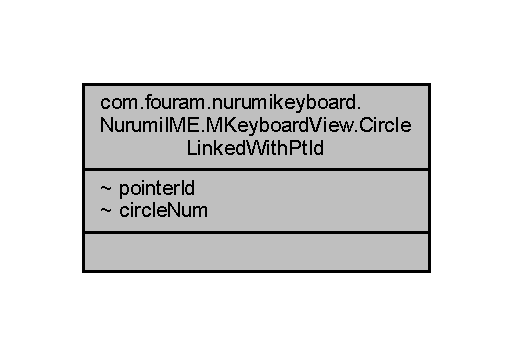
\includegraphics[width=246pt]{classcom_1_1fouram_1_1nurumikeyboard_1_1_nurumi_i_m_e_1_1_m_keyboard_view_1_1_circle_linked_with_pt_id__coll__graph}
\end{center}
\end{figure}


\subsection{Detailed Description}
\hyperlink{namespacecom_1_1fouram_1_1nurumikeyboard_1_1_nurumi_i_m_e}{com.\+fouram.\+nurumikeyboard.\+Nurumi\+I\+M\+E} ~\newline
 �� \hyperlink{_m_keyboard_view_8java}{M\+Keyboard\+View.\+java} \hypertarget{classcom_1_1fouram_1_1nurumikeyboard_1_1_nurumi_i_m_e_1_1_m_keyboard_view_1_1_pt_id_linked_with_pt_index_Class}{}\subsection{information}\label{classcom_1_1fouram_1_1nurumikeyboard_1_1_nurumi_i_m_e_1_1_m_keyboard_view_1_1_pt_id_linked_with_pt_index_Class}
\begin{TabularC}{2}
\hline
\rowcolor{lightgray}\PBS\centering {\bf Item }&{\bf Contents  }\\\cline{1-2}
\PBS\centering Company &4\+:00 A.\+M. \\\cline{1-2}
\PBS\centering Author &Park, Hyung Soon \\\cline{1-2}
\PBS\centering Date &2015. 3. 26. \\\cline{1-2}
\end{TabularC}
\hypertarget{classcom_1_1fouram_1_1nurumikeyboard_1_1_nurumi_i_m_e_1_1_m_keyboard_view_1_1_pt_id_linked_with_pt_index_Description}{}\subsection{Description}\label{classcom_1_1fouram_1_1nurumikeyboard_1_1_nurumi_i_m_e_1_1_m_keyboard_view_1_1_pt_id_linked_with_pt_index_Description}

\begin{DoxyItemize}
\item This class will bind pointer\+I\+D with circle\+Num.~\newline

\end{DoxyItemize}

Definition at line 83 of file M\+Keyboard\+View.\+java.



The documentation for this class was generated from the following file\+:\begin{DoxyCompactItemize}
\item 
src/com/fouram/nurumikeyboard/\+Nurumi\+I\+M\+E/\hyperlink{_m_keyboard_view_8java}{M\+Keyboard\+View.\+java}\end{DoxyCompactItemize}

\hypertarget{classcom_1_1fouram_1_1nurumikeyboard_1_1_nurumi_i_m_e_1_1_m_keyboard_view}{}\section{com.\+fouram.\+nurumikeyboard.\+Nurumi\+I\+M\+E.\+M\+Keyboard\+View Class Reference}
\label{classcom_1_1fouram_1_1nurumikeyboard_1_1_nurumi_i_m_e_1_1_m_keyboard_view}\index{com.\+fouram.\+nurumikeyboard.\+Nurumi\+I\+M\+E.\+M\+Keyboard\+View@{com.\+fouram.\+nurumikeyboard.\+Nurumi\+I\+M\+E.\+M\+Keyboard\+View}}


Inheritance diagram for com.\+fouram.\+nurumikeyboard.\+Nurumi\+I\+M\+E.\+M\+Keyboard\+View\+:
\nopagebreak
\begin{figure}[H]
\begin{center}
\leavevmode
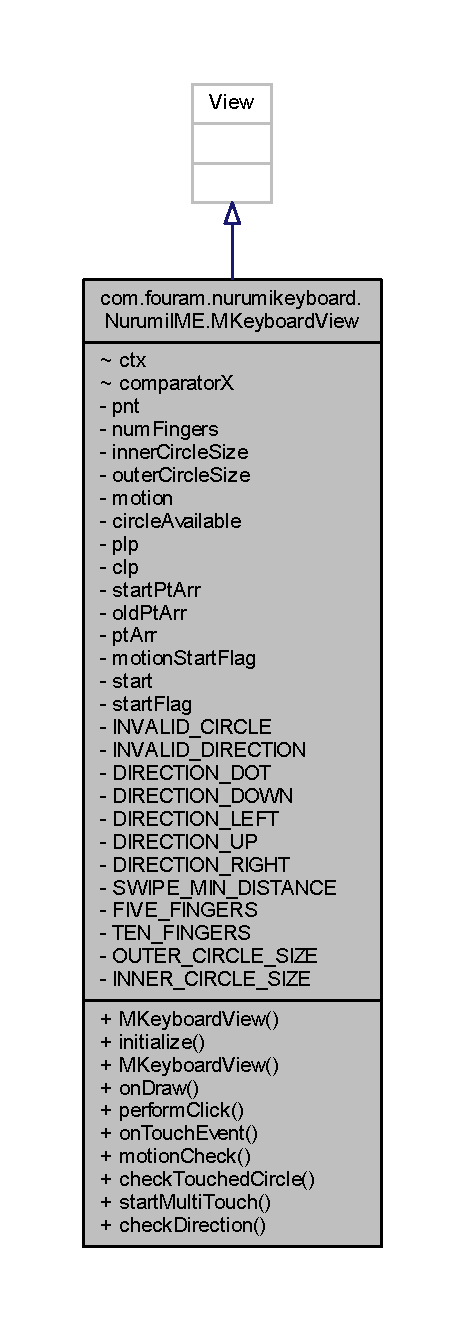
\includegraphics[height=550pt]{classcom_1_1fouram_1_1nurumikeyboard_1_1_nurumi_i_m_e_1_1_m_keyboard_view__inherit__graph}
\end{center}
\end{figure}


Collaboration diagram for com.\+fouram.\+nurumikeyboard.\+Nurumi\+I\+M\+E.\+M\+Keyboard\+View\+:
\nopagebreak
\begin{figure}[H]
\begin{center}
\leavevmode
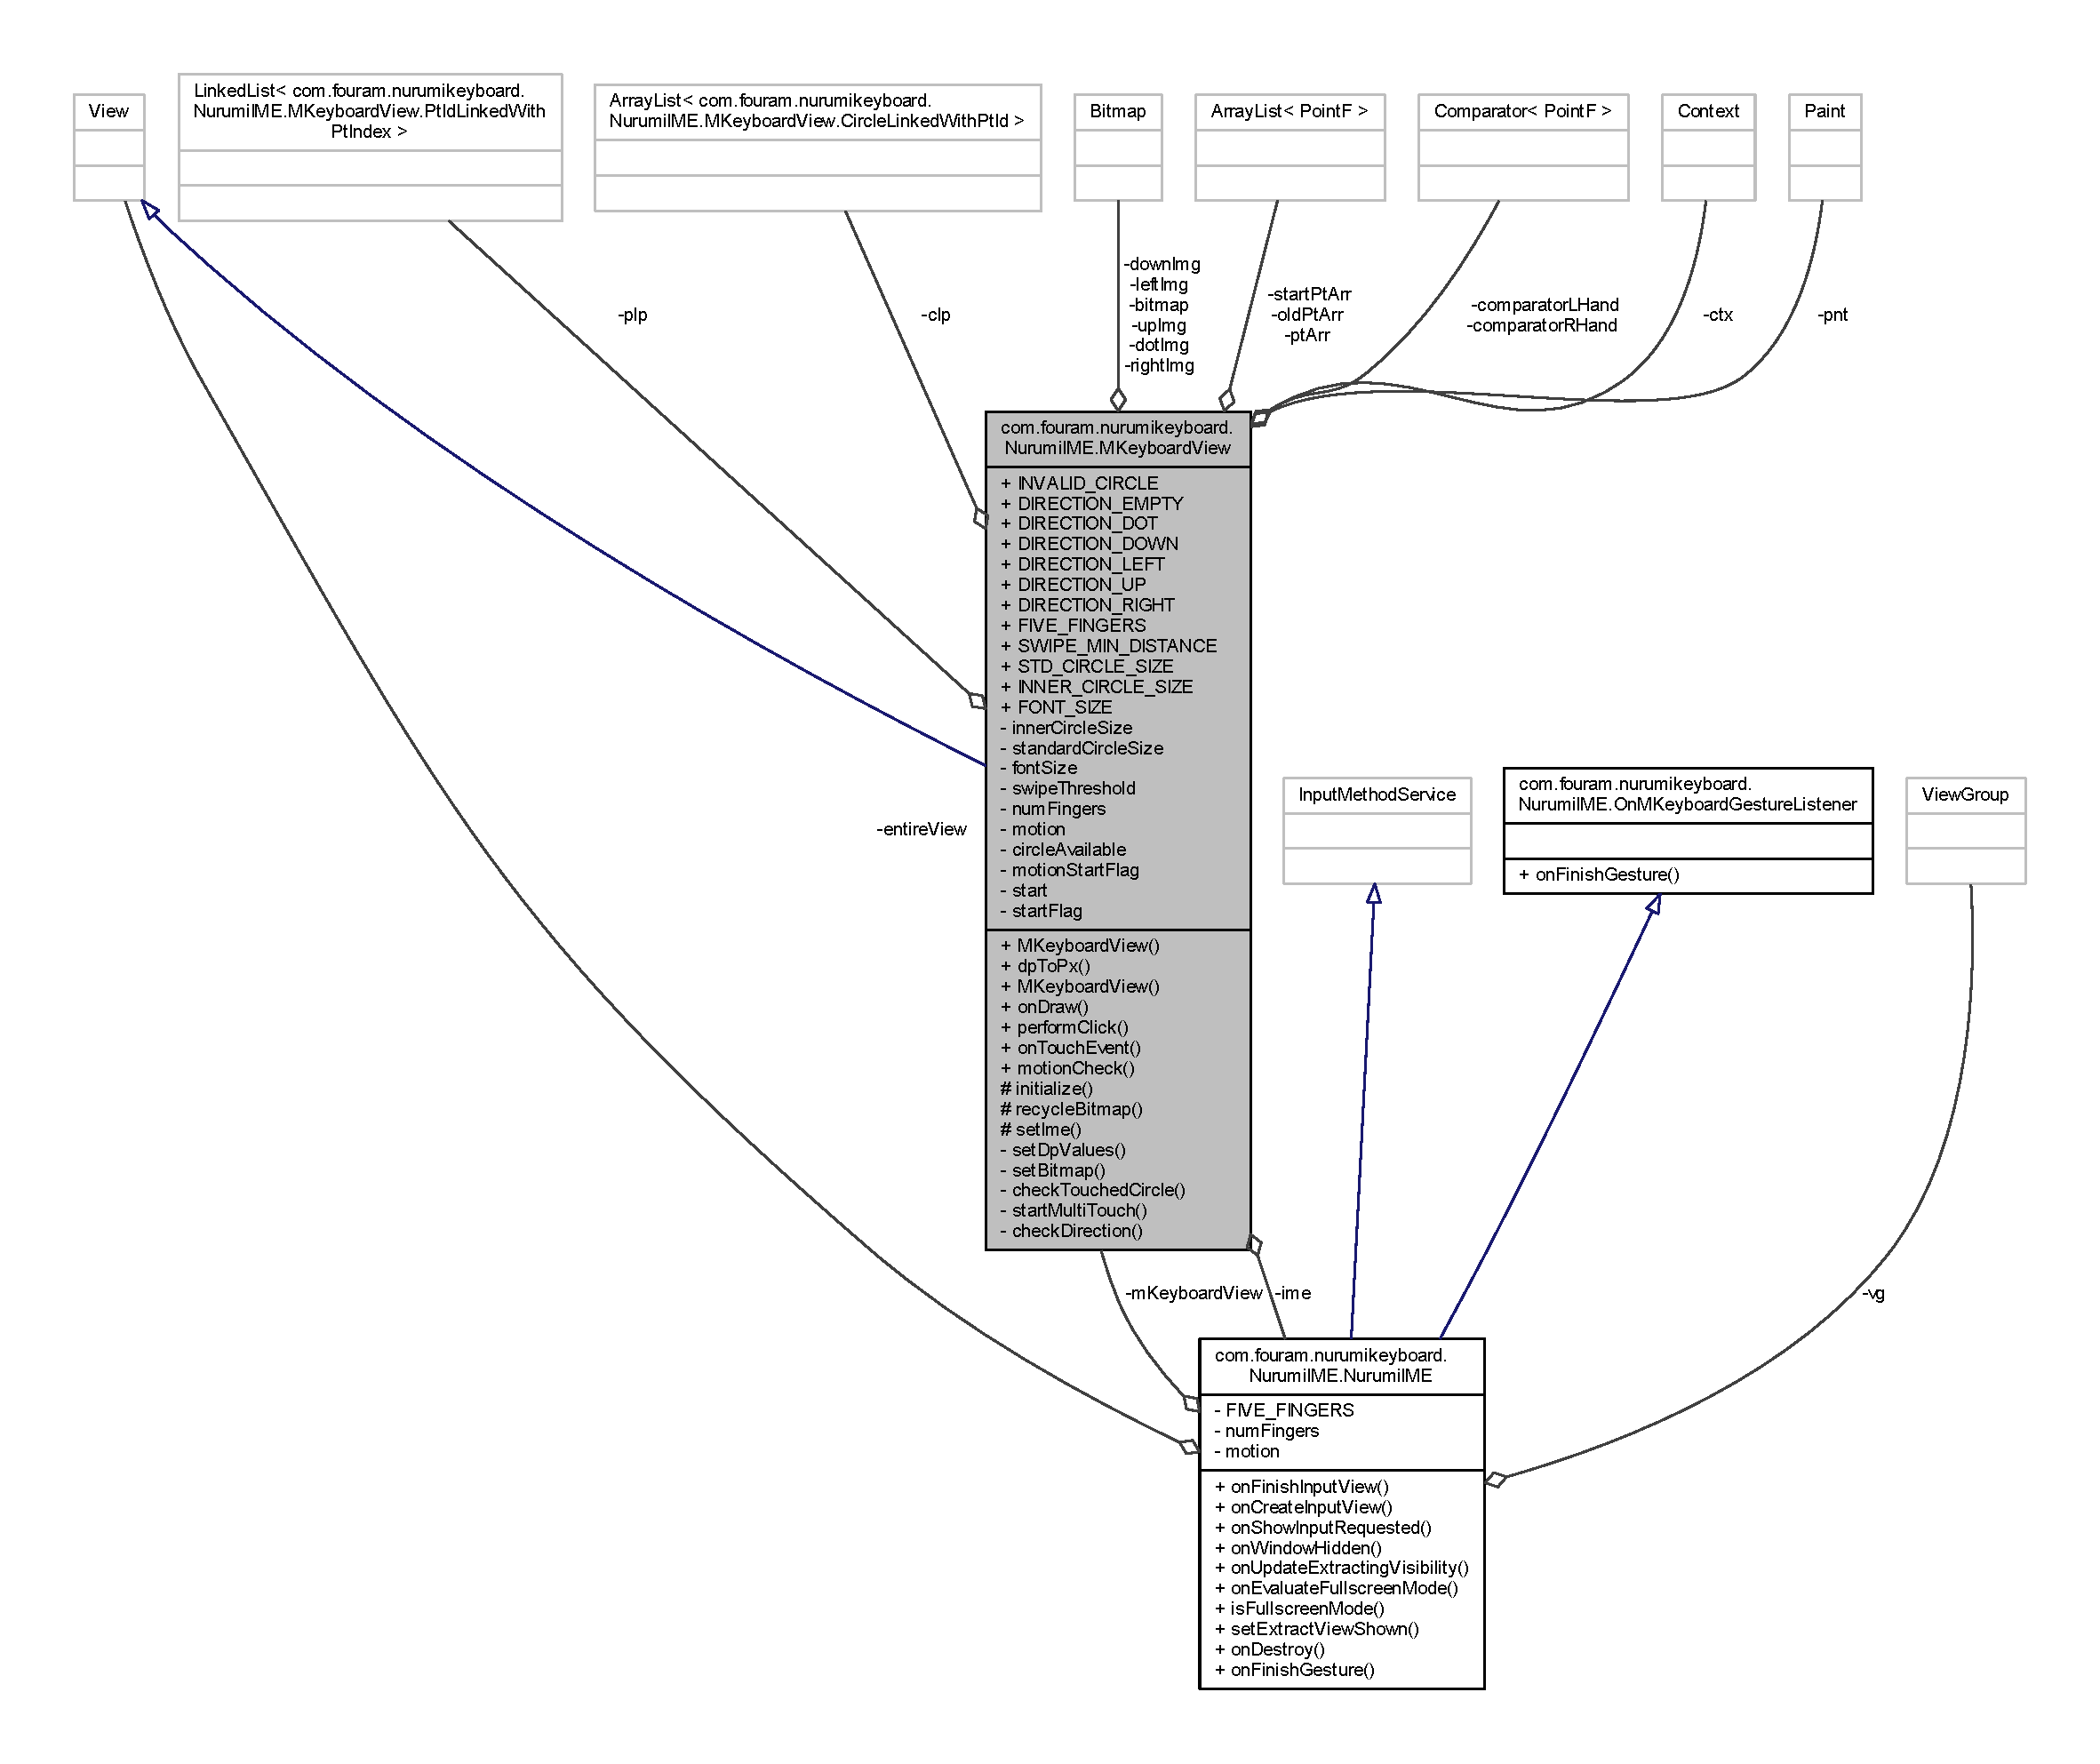
\includegraphics[width=350pt]{classcom_1_1fouram_1_1nurumikeyboard_1_1_nurumi_i_m_e_1_1_m_keyboard_view__coll__graph}
\end{center}
\end{figure}
\subsection*{Classes}
\begin{DoxyCompactItemize}
\item 
class \hyperlink{classcom_1_1fouram_1_1nurumikeyboard_1_1_nurumi_i_m_e_1_1_m_keyboard_view_1_1_circle_linked_with_pt_id}{Circle\+Linked\+With\+Pt\+Id}
\item 
class \hyperlink{classcom_1_1fouram_1_1nurumikeyboard_1_1_nurumi_i_m_e_1_1_m_keyboard_view_1_1_pt_id_linked_with_pt_index}{Pt\+Id\+Linked\+With\+Pt\+Index}
\end{DoxyCompactItemize}
\subsection*{Public Member Functions}
\begin{DoxyCompactItemize}
\item 
\hyperlink{classcom_1_1fouram_1_1nurumikeyboard_1_1_nurumi_i_m_e_1_1_m_keyboard_view_a970fc12bcbc4830bea85945fd4909edd}{M\+Keyboard\+View} (Context context, Attribute\+Set attrs)
\item 
void \hyperlink{classcom_1_1fouram_1_1nurumikeyboard_1_1_nurumi_i_m_e_1_1_m_keyboard_view_a536f8d1527df8c5013dc66d253ac5dae}{initialize} ()
\begin{DoxyCompactList}\small\item\em Function information \+: Initialize function. \end{DoxyCompactList}\item 
\hyperlink{classcom_1_1fouram_1_1nurumikeyboard_1_1_nurumi_i_m_e_1_1_m_keyboard_view_a565bb11cbc920cca01f533beb7468419}{M\+Keyboard\+View} (Context context)
\item 
void \hyperlink{classcom_1_1fouram_1_1nurumikeyboard_1_1_nurumi_i_m_e_1_1_m_keyboard_view_a775825f89451ffcdacfbceb7fa201d48}{on\+Draw} (Canvas canvas)
\item 
boolean \hyperlink{classcom_1_1fouram_1_1nurumikeyboard_1_1_nurumi_i_m_e_1_1_m_keyboard_view_a6af440ca9c6043f361e51ead2e95620a}{perform\+Click} ()
\item 
boolean \hyperlink{classcom_1_1fouram_1_1nurumikeyboard_1_1_nurumi_i_m_e_1_1_m_keyboard_view_a18509488a51daf21c5b16841aaa035c9}{on\+Touch\+Event} (Motion\+Event e)
\begin{DoxyCompactList}\small\item\em Function information \+: Touch event method. \end{DoxyCompactList}\item 
void \hyperlink{classcom_1_1fouram_1_1nurumikeyboard_1_1_nurumi_i_m_e_1_1_m_keyboard_view_a657f24f9888d141266179c6dc971103f}{motion\+Check} ()
\begin{DoxyCompactList}\small\item\em Function information \+: Motion checking method. \end{DoxyCompactList}\item 
int \hyperlink{classcom_1_1fouram_1_1nurumikeyboard_1_1_nurumi_i_m_e_1_1_m_keyboard_view_ad7701634206a8ad8fb6ad5bc72fc39d1}{check\+Touched\+Circle} (int x, int y)
\begin{DoxyCompactList}\small\item\em Function information \+: Find touched circle. \end{DoxyCompactList}\item 
boolean \hyperlink{classcom_1_1fouram_1_1nurumikeyboard_1_1_nurumi_i_m_e_1_1_m_keyboard_view_a2e05b77b14ceb804926bc33e9e3e88fa}{start\+Multi\+Touch} (Motion\+Event e)
\begin{DoxyCompactList}\small\item\em Function information \+: Start multi touch recognition. \end{DoxyCompactList}\item 
void \hyperlink{classcom_1_1fouram_1_1nurumikeyboard_1_1_nurumi_i_m_e_1_1_m_keyboard_view_aa548466053ead7d81890a197df4e0665}{check\+Direction} (\hyperlink{classcom_1_1fouram_1_1nurumikeyboard_1_1_nurumi_i_m_e_1_1_m_keyboard_view_1_1_pt_id_linked_with_pt_index}{Pt\+Id\+Linked\+With\+Pt\+Index} pp, Point\+F pt)
\begin{DoxyCompactList}\small\item\em Function information \+: Check the direction of movement of pointers. \end{DoxyCompactList}\end{DoxyCompactItemize}
\subsection*{Private Attributes}
\begin{DoxyCompactItemize}
\item 
Paint \hyperlink{classcom_1_1fouram_1_1nurumikeyboard_1_1_nurumi_i_m_e_1_1_m_keyboard_view_a113cc5cd53707a1d2df822c487dcbe8c}{pnt}
\item 
int \hyperlink{classcom_1_1fouram_1_1nurumikeyboard_1_1_nurumi_i_m_e_1_1_m_keyboard_view_af2f59861ed61c6357020e1350be33a5a}{num\+Fingers}
\item 
int \hyperlink{classcom_1_1fouram_1_1nurumikeyboard_1_1_nurumi_i_m_e_1_1_m_keyboard_view_aa8664e099a4f809a3abf8cdae1c4c393}{inner\+Circle\+Size}
\item 
int \hyperlink{classcom_1_1fouram_1_1nurumikeyboard_1_1_nurumi_i_m_e_1_1_m_keyboard_view_a92db4315e015e0c892d2c324557c599c}{outer\+Circle\+Size}
\item 
int\mbox{[}$\,$\mbox{]} \hyperlink{classcom_1_1fouram_1_1nurumikeyboard_1_1_nurumi_i_m_e_1_1_m_keyboard_view_a33b834fb352211295449e26a9f495807}{motion}
\item 
boolean\mbox{[}$\,$\mbox{]} \hyperlink{classcom_1_1fouram_1_1nurumikeyboard_1_1_nurumi_i_m_e_1_1_m_keyboard_view_a087c107ffdad9ad25e5d28bd003a15c9}{circle\+Available}
\item 
Linked\+List$<$ \hyperlink{classcom_1_1fouram_1_1nurumikeyboard_1_1_nurumi_i_m_e_1_1_m_keyboard_view_1_1_pt_id_linked_with_pt_index}{Pt\+Id\+Linked\+With\+Pt\+Index} $>$ \hyperlink{classcom_1_1fouram_1_1nurumikeyboard_1_1_nurumi_i_m_e_1_1_m_keyboard_view_a759f646f0682c75387d7a0d8cd3d8cbf}{plp}
\item 
Array\+List$<$ \hyperlink{classcom_1_1fouram_1_1nurumikeyboard_1_1_nurumi_i_m_e_1_1_m_keyboard_view_1_1_circle_linked_with_pt_id}{Circle\+Linked\+With\+Pt\+Id} $>$ \hyperlink{classcom_1_1fouram_1_1nurumikeyboard_1_1_nurumi_i_m_e_1_1_m_keyboard_view_adba837582df67530dd4a9d93fc1825a9}{clp}
\item 
Array\+List$<$ Point\+F $>$ \hyperlink{classcom_1_1fouram_1_1nurumikeyboard_1_1_nurumi_i_m_e_1_1_m_keyboard_view_aff948c186aac098473fed848c94fc086}{start\+Pt\+Arr}
\item 
Array\+List$<$ Point\+F $>$ \hyperlink{classcom_1_1fouram_1_1nurumikeyboard_1_1_nurumi_i_m_e_1_1_m_keyboard_view_ac7da84e25f4d6414da9023da4a8d3ffa}{old\+Pt\+Arr}
\item 
Array\+List$<$ Point\+F $>$ \hyperlink{classcom_1_1fouram_1_1nurumikeyboard_1_1_nurumi_i_m_e_1_1_m_keyboard_view_a803bbeb52f830df78ab726874a9e7e17}{pt\+Arr}
\item 
boolean \hyperlink{classcom_1_1fouram_1_1nurumikeyboard_1_1_nurumi_i_m_e_1_1_m_keyboard_view_a0ac7b4552f63165d0447bbe12a55b813}{motion\+Start\+Flag}
\item 
boolean \hyperlink{classcom_1_1fouram_1_1nurumikeyboard_1_1_nurumi_i_m_e_1_1_m_keyboard_view_a13bdd74ac521ef4655cd139c647de466}{start}
\item 
boolean \hyperlink{classcom_1_1fouram_1_1nurumikeyboard_1_1_nurumi_i_m_e_1_1_m_keyboard_view_ace13bdd1bb9cdcc07b7c4f6345d51670}{start\+Flag}
\end{DoxyCompactItemize}
\subsection*{Static Private Attributes}
\begin{DoxyCompactItemize}
\item 
static final int \hyperlink{classcom_1_1fouram_1_1nurumikeyboard_1_1_nurumi_i_m_e_1_1_m_keyboard_view_a595dcf17ea60a02818d53551cd1dbe4d}{I\+N\+V\+A\+L\+I\+D\+\_\+\+C\+I\+R\+C\+L\+E} = -\/1
\item 
static final int \hyperlink{classcom_1_1fouram_1_1nurumikeyboard_1_1_nurumi_i_m_e_1_1_m_keyboard_view_af02d80d6fbd44cae54c67a461858a5cd}{I\+N\+V\+A\+L\+I\+D\+\_\+\+D\+I\+R\+E\+C\+T\+I\+O\+N} = -\/1
\item 
static final int \hyperlink{classcom_1_1fouram_1_1nurumikeyboard_1_1_nurumi_i_m_e_1_1_m_keyboard_view_ab3af4b0b8e75ae26bc33534c1736c701}{D\+I\+R\+E\+C\+T\+I\+O\+N\+\_\+\+D\+O\+T} = 0
\item 
static final int \hyperlink{classcom_1_1fouram_1_1nurumikeyboard_1_1_nurumi_i_m_e_1_1_m_keyboard_view_a244ae46f473dfa5074d64a5af1e90ecf}{D\+I\+R\+E\+C\+T\+I\+O\+N\+\_\+\+D\+O\+W\+N} = 1
\item 
static final int \hyperlink{classcom_1_1fouram_1_1nurumikeyboard_1_1_nurumi_i_m_e_1_1_m_keyboard_view_ad72ab456e489e8c3e860bfa1d094c057}{D\+I\+R\+E\+C\+T\+I\+O\+N\+\_\+\+L\+E\+F\+T} = 2
\item 
static final int \hyperlink{classcom_1_1fouram_1_1nurumikeyboard_1_1_nurumi_i_m_e_1_1_m_keyboard_view_a720a8b5a9553d6b9bc0fcb94bf387eaa}{D\+I\+R\+E\+C\+T\+I\+O\+N\+\_\+\+U\+P} = 3
\item 
static final int \hyperlink{classcom_1_1fouram_1_1nurumikeyboard_1_1_nurumi_i_m_e_1_1_m_keyboard_view_a94f48baa64fed71b4f1f316958ba2a3e}{D\+I\+R\+E\+C\+T\+I\+O\+N\+\_\+\+R\+I\+G\+H\+T} = 4
\item 
static final int \hyperlink{classcom_1_1fouram_1_1nurumikeyboard_1_1_nurumi_i_m_e_1_1_m_keyboard_view_a6e09544be36903fcc2395fecb6fd3dae}{S\+W\+I\+P\+E\+\_\+\+M\+I\+N\+\_\+\+D\+I\+S\+T\+A\+N\+C\+E} = 140
\item 
static final int \hyperlink{classcom_1_1fouram_1_1nurumikeyboard_1_1_nurumi_i_m_e_1_1_m_keyboard_view_a61263eb41eed8667a83505e8771c5b23}{F\+I\+V\+E\+\_\+\+F\+I\+N\+G\+E\+R\+S} = 5
\item 
static final int \hyperlink{classcom_1_1fouram_1_1nurumikeyboard_1_1_nurumi_i_m_e_1_1_m_keyboard_view_aa3081bef03a1aa0af4b6ec3496b041cb}{T\+E\+N\+\_\+\+F\+I\+N\+G\+E\+R\+S} = 10
\item 
static final int \hyperlink{classcom_1_1fouram_1_1nurumikeyboard_1_1_nurumi_i_m_e_1_1_m_keyboard_view_aabab90ddcaeedf63348d892614c9d168}{O\+U\+T\+E\+R\+\_\+\+C\+I\+R\+C\+L\+E\+\_\+\+S\+I\+Z\+E} = 140
\item 
static final int \hyperlink{classcom_1_1fouram_1_1nurumikeyboard_1_1_nurumi_i_m_e_1_1_m_keyboard_view_af7119aa21410f68aa856612add4d464c}{I\+N\+N\+E\+R\+\_\+\+C\+I\+R\+C\+L\+E\+\_\+\+S\+I\+Z\+E} = 100
\end{DoxyCompactItemize}


\subsection{Detailed Description}
\hyperlink{namespacecom_1_1fouram_1_1nurumikeyboard_1_1_nurumi_i_m_e}{com.\+fouram.\+nurumikeyboard.\+Nurumi\+I\+M\+E} ~\newline
 �� \hyperlink{_m_keyboard_view_8java}{M\+Keyboard\+View.\+java} \hypertarget{classcom_1_1fouram_1_1nurumikeyboard_1_1_nurumi_i_m_e_1_1_m_keyboard_view_1_1_pt_id_linked_with_pt_index_Class}{}\subsection{information}\label{classcom_1_1fouram_1_1nurumikeyboard_1_1_nurumi_i_m_e_1_1_m_keyboard_view_1_1_pt_id_linked_with_pt_index_Class}
\begin{TabularC}{2}
\hline
\rowcolor{lightgray}\PBS\centering {\bf Item }&{\bf Contents  }\\\cline{1-2}
\PBS\centering Company &4\+:00 A.\+M. \\\cline{1-2}
\PBS\centering Author &Park, Hyung Soon \\\cline{1-2}
\PBS\centering Date &2015. 3. 26. \\\cline{1-2}
\end{TabularC}
\hypertarget{classcom_1_1fouram_1_1nurumikeyboard_1_1_nurumi_i_m_e_1_1_m_keyboard_view_1_1_pt_id_linked_with_pt_index_Description}{}\subsection{Description}\label{classcom_1_1fouram_1_1nurumikeyboard_1_1_nurumi_i_m_e_1_1_m_keyboard_view_1_1_pt_id_linked_with_pt_index_Description}

\begin{DoxyItemize}
\item This file is for the view of motion keyboard.~\newline

\item This view will popup when user~\newline
 put cursor in textbox,~\newline
 \hyperlink{namespacecom_1_1fouram_1_1nurumikeyboard_1_1_nurumi_i_m_e}{com.\+fouram.\+nurumikeyboard.\+Nurumi\+I\+M\+E} ~\newline
 �� \hyperlink{_m_keyboard_view_8java}{M\+Keyboard\+View.\+java} 
\end{DoxyItemize}\hypertarget{classcom_1_1fouram_1_1nurumikeyboard_1_1_nurumi_i_m_e_1_1_m_keyboard_view_1_1_pt_id_linked_with_pt_index_Class}{}\subsection{information}\label{classcom_1_1fouram_1_1nurumikeyboard_1_1_nurumi_i_m_e_1_1_m_keyboard_view_1_1_pt_id_linked_with_pt_index_Class}
\begin{TabularC}{2}
\hline
\rowcolor{lightgray}\PBS\centering {\bf Item }&{\bf Contents  }\\\cline{1-2}
\PBS\centering Company &4\+:00 A.\+M. \\\cline{1-2}
\PBS\centering Author &Park, Hyung Soon \\\cline{1-2}
\PBS\centering Date &2015. 3. 26. \\\cline{1-2}
\end{TabularC}
\hypertarget{classcom_1_1fouram_1_1nurumikeyboard_1_1_nurumi_i_m_e_1_1_m_keyboard_view_1_1_pt_id_linked_with_pt_index_Description}{}\subsection{Description}\label{classcom_1_1fouram_1_1nurumikeyboard_1_1_nurumi_i_m_e_1_1_m_keyboard_view_1_1_pt_id_linked_with_pt_index_Description}

\begin{DoxyItemize}
\item View of motion keyboard~\newline

\end{DoxyItemize}

Definition at line 47 of file M\+Keyboard\+View.\+java.



\subsection{Constructor \& Destructor Documentation}
\hypertarget{classcom_1_1fouram_1_1nurumikeyboard_1_1_nurumi_i_m_e_1_1_m_keyboard_view_a970fc12bcbc4830bea85945fd4909edd}{}\index{com\+::fouram\+::nurumikeyboard\+::\+Nurumi\+I\+M\+E\+::\+M\+Keyboard\+View@{com\+::fouram\+::nurumikeyboard\+::\+Nurumi\+I\+M\+E\+::\+M\+Keyboard\+View}!M\+Keyboard\+View@{M\+Keyboard\+View}}
\index{M\+Keyboard\+View@{M\+Keyboard\+View}!com\+::fouram\+::nurumikeyboard\+::\+Nurumi\+I\+M\+E\+::\+M\+Keyboard\+View@{com\+::fouram\+::nurumikeyboard\+::\+Nurumi\+I\+M\+E\+::\+M\+Keyboard\+View}}
\subsubsection[{M\+Keyboard\+View}]{\setlength{\rightskip}{0pt plus 5cm}com.\+fouram.\+nurumikeyboard.\+Nurumi\+I\+M\+E.\+M\+Keyboard\+View.\+M\+Keyboard\+View (
\begin{DoxyParamCaption}
\item[{Context}]{context, }
\item[{Attribute\+Set}]{attrs}
\end{DoxyParamCaption}
)}\label{classcom_1_1fouram_1_1nurumikeyboard_1_1_nurumi_i_m_e_1_1_m_keyboard_view_a970fc12bcbc4830bea85945fd4909edd}


Definition at line 153 of file M\+Keyboard\+View.\+java.


\begin{DoxyCode}
153                                                               \{
154         super(context, attrs);
155         this.ctx = context;
156         \hyperlink{classcom_1_1fouram_1_1nurumikeyboard_1_1_nurumi_i_m_e_1_1_m_keyboard_view_a536f8d1527df8c5013dc66d253ac5dae}{initialize}();     
157     \}
\end{DoxyCode}


Here is the call graph for this function\+:
\nopagebreak
\begin{figure}[H]
\begin{center}
\leavevmode
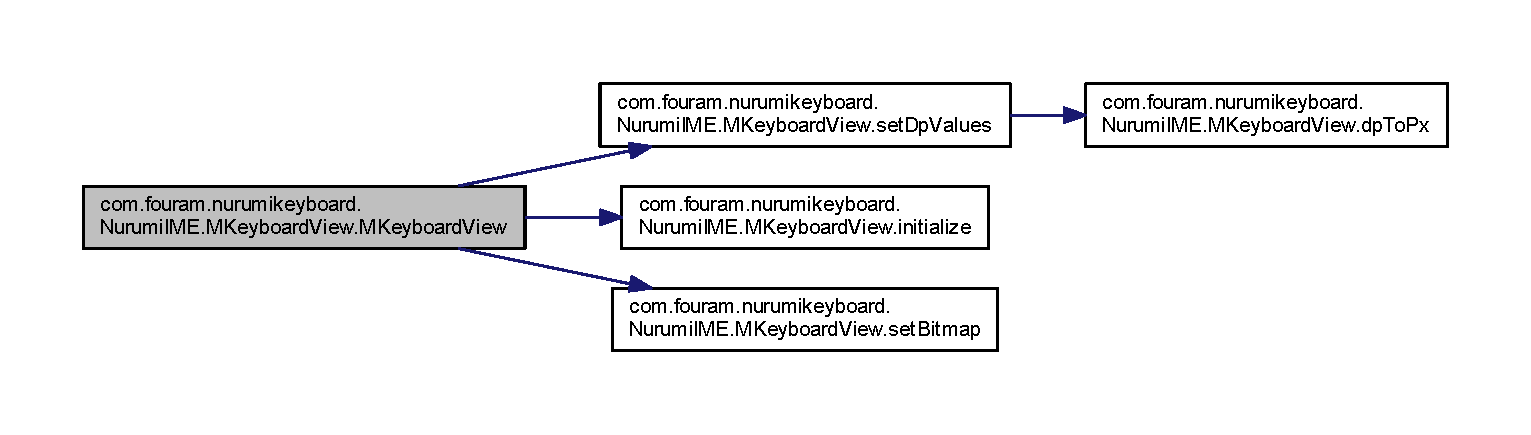
\includegraphics[width=350pt]{classcom_1_1fouram_1_1nurumikeyboard_1_1_nurumi_i_m_e_1_1_m_keyboard_view_a970fc12bcbc4830bea85945fd4909edd_cgraph}
\end{center}
\end{figure}


\hypertarget{classcom_1_1fouram_1_1nurumikeyboard_1_1_nurumi_i_m_e_1_1_m_keyboard_view_a565bb11cbc920cca01f533beb7468419}{}\index{com\+::fouram\+::nurumikeyboard\+::\+Nurumi\+I\+M\+E\+::\+M\+Keyboard\+View@{com\+::fouram\+::nurumikeyboard\+::\+Nurumi\+I\+M\+E\+::\+M\+Keyboard\+View}!M\+Keyboard\+View@{M\+Keyboard\+View}}
\index{M\+Keyboard\+View@{M\+Keyboard\+View}!com\+::fouram\+::nurumikeyboard\+::\+Nurumi\+I\+M\+E\+::\+M\+Keyboard\+View@{com\+::fouram\+::nurumikeyboard\+::\+Nurumi\+I\+M\+E\+::\+M\+Keyboard\+View}}
\subsubsection[{M\+Keyboard\+View}]{\setlength{\rightskip}{0pt plus 5cm}com.\+fouram.\+nurumikeyboard.\+Nurumi\+I\+M\+E.\+M\+Keyboard\+View.\+M\+Keyboard\+View (
\begin{DoxyParamCaption}
\item[{Context}]{context}
\end{DoxyParamCaption}
)}\label{classcom_1_1fouram_1_1nurumikeyboard_1_1_nurumi_i_m_e_1_1_m_keyboard_view_a565bb11cbc920cca01f533beb7468419}


Definition at line 200 of file M\+Keyboard\+View.\+java.


\begin{DoxyCode}
200                                           \{
201         super(context);
202         this.ctx = context;
203     \}
\end{DoxyCode}


\subsection{Member Function Documentation}
\hypertarget{classcom_1_1fouram_1_1nurumikeyboard_1_1_nurumi_i_m_e_1_1_m_keyboard_view_aa548466053ead7d81890a197df4e0665}{}\index{com\+::fouram\+::nurumikeyboard\+::\+Nurumi\+I\+M\+E\+::\+M\+Keyboard\+View@{com\+::fouram\+::nurumikeyboard\+::\+Nurumi\+I\+M\+E\+::\+M\+Keyboard\+View}!check\+Direction@{check\+Direction}}
\index{check\+Direction@{check\+Direction}!com\+::fouram\+::nurumikeyboard\+::\+Nurumi\+I\+M\+E\+::\+M\+Keyboard\+View@{com\+::fouram\+::nurumikeyboard\+::\+Nurumi\+I\+M\+E\+::\+M\+Keyboard\+View}}
\subsubsection[{check\+Direction}]{\setlength{\rightskip}{0pt plus 5cm}com.\+fouram.\+nurumikeyboard.\+Nurumi\+I\+M\+E.\+M\+Keyboard\+View.\+check\+Direction (
\begin{DoxyParamCaption}
\item[{{\bf Pt\+Id\+Linked\+With\+Pt\+Index}}]{pp, }
\item[{Point\+F}]{pt}
\end{DoxyParamCaption}
)}\label{classcom_1_1fouram_1_1nurumikeyboard_1_1_nurumi_i_m_e_1_1_m_keyboard_view_aa548466053ead7d81890a197df4e0665}


Function information \+: Check the direction of movement of pointers. 

\begin{DoxyRemark}{Remarks}

\begin{DoxyItemize}
\item Description \+: Calculate the moved distances of pointers and save them in \textquotesingle{}motion\textquotesingle{} array. 
\end{DoxyItemize}
\end{DoxyRemark}

\begin{DoxyParams}{Parameters}
{\em pp} & \+: List of class which has Pointer I\+D and Pointer Index to link them. \\
\hline
{\em pt} & \+: Grid of currently moving pointer.\\
\hline
\end{DoxyParams}

\begin{DoxyCode}
\textcolor{comment}{// core code}
\end{DoxyCode}
 

Definition at line 556 of file M\+Keyboard\+View.\+java.


\begin{DoxyCode}
557     \{
558         CircleLinkedWithPtId cp = \textcolor{keyword}{new} CircleLinkedWithPtId();
559         \textcolor{keywordflow}{for}(\textcolor{keywordtype}{int} i=0; i<\hyperlink{classcom_1_1fouram_1_1nurumikeyboard_1_1_nurumi_i_m_e_1_1_m_keyboard_view_af2f59861ed61c6357020e1350be33a5a}{numFingers}; i++)
560         \{
561             \textcolor{keywordflow}{if}(\hyperlink{classcom_1_1fouram_1_1nurumikeyboard_1_1_nurumi_i_m_e_1_1_m_keyboard_view_adba837582df67530dd4a9d93fc1825a9}{clp}.size() <= i)
562                 \textcolor{keywordflow}{return};
563             cp = \hyperlink{classcom_1_1fouram_1_1nurumikeyboard_1_1_nurumi_i_m_e_1_1_m_keyboard_view_adba837582df67530dd4a9d93fc1825a9}{clp}.get(i);
564             \textcolor{keywordflow}{if}(pp.pointerId == cp.pointerId)
565                 \textcolor{keywordflow}{break};
566         \}
567         
568         PointF oldPt = \textcolor{keyword}{new} PointF();
569         \textcolor{keywordtype}{int} circleNum = -1;
570         \textcolor{keywordflow}{for}(\textcolor{keywordtype}{int} i=0; i<\hyperlink{classcom_1_1fouram_1_1nurumikeyboard_1_1_nurumi_i_m_e_1_1_m_keyboard_view_af2f59861ed61c6357020e1350be33a5a}{numFingers}; i++)
571         \{
572             \textcolor{keywordflow}{if}(\hyperlink{classcom_1_1fouram_1_1nurumikeyboard_1_1_nurumi_i_m_e_1_1_m_keyboard_view_ac7da84e25f4d6414da9023da4a8d3ffa}{oldPtArr}.size() <= i)
573                 \textcolor{keywordflow}{break};
574             oldPt = \hyperlink{classcom_1_1fouram_1_1nurumikeyboard_1_1_nurumi_i_m_e_1_1_m_keyboard_view_ac7da84e25f4d6414da9023da4a8d3ffa}{oldPtArr}.get(i);
575             circleNum = \hyperlink{classcom_1_1fouram_1_1nurumikeyboard_1_1_nurumi_i_m_e_1_1_m_keyboard_view_ad7701634206a8ad8fb6ad5bc72fc39d1}{checkTouchedCircle}((\textcolor{keywordtype}{int})oldPt.x, (\textcolor{keywordtype}{int})oldPt.y);
576             \textcolor{keywordflow}{if}(cp.circleNum == circleNum)
577                 \textcolor{keywordflow}{break};
578         \}
579         \textcolor{keywordflow}{if}(circleNum == -1) \textcolor{keywordflow}{return};
580         
581         \textcolor{keywordtype}{float} distanceX = oldPt.x - pt.x;
582         \textcolor{keywordtype}{float} distanceY = oldPt.y - pt.y;
583         
584         \textcolor{keywordflow}{if}( Math.abs(distanceX) < \hyperlink{classcom_1_1fouram_1_1nurumikeyboard_1_1_nurumi_i_m_e_1_1_m_keyboard_view_a6e09544be36903fcc2395fecb6fd3dae}{SWIPE\_MIN\_DISTANCE} && Math.abs(distanceY) < 
      \hyperlink{classcom_1_1fouram_1_1nurumikeyboard_1_1_nurumi_i_m_e_1_1_m_keyboard_view_a6e09544be36903fcc2395fecb6fd3dae}{SWIPE\_MIN\_DISTANCE} )
585             \hyperlink{classcom_1_1fouram_1_1nurumikeyboard_1_1_nurumi_i_m_e_1_1_m_keyboard_view_a33b834fb352211295449e26a9f495807}{motion}[circleNum-1] = \hyperlink{classcom_1_1fouram_1_1nurumikeyboard_1_1_nurumi_i_m_e_1_1_m_keyboard_view_ab3af4b0b8e75ae26bc33534c1736c701}{DIRECTION\_DOT};
586         \textcolor{keywordflow}{else} \textcolor{keywordflow}{if}( Math.abs(distanceX) > \hyperlink{classcom_1_1fouram_1_1nurumikeyboard_1_1_nurumi_i_m_e_1_1_m_keyboard_view_a6e09544be36903fcc2395fecb6fd3dae}{SWIPE\_MIN\_DISTANCE} && Math.abs(distanceY) > 
      \hyperlink{classcom_1_1fouram_1_1nurumikeyboard_1_1_nurumi_i_m_e_1_1_m_keyboard_view_a6e09544be36903fcc2395fecb6fd3dae}{SWIPE\_MIN\_DISTANCE} )
587             \hyperlink{classcom_1_1fouram_1_1nurumikeyboard_1_1_nurumi_i_m_e_1_1_m_keyboard_view_a33b834fb352211295449e26a9f495807}{motion}[circleNum-1] = \hyperlink{classcom_1_1fouram_1_1nurumikeyboard_1_1_nurumi_i_m_e_1_1_m_keyboard_view_af02d80d6fbd44cae54c67a461858a5cd}{INVALID\_DIRECTION};
588         \textcolor{keywordflow}{else} \textcolor{keywordflow}{if}( Math.abs(distanceX) > \hyperlink{classcom_1_1fouram_1_1nurumikeyboard_1_1_nurumi_i_m_e_1_1_m_keyboard_view_a6e09544be36903fcc2395fecb6fd3dae}{SWIPE\_MIN\_DISTANCE} && distanceX > 0)
589             \hyperlink{classcom_1_1fouram_1_1nurumikeyboard_1_1_nurumi_i_m_e_1_1_m_keyboard_view_a33b834fb352211295449e26a9f495807}{motion}[circleNum-1] = \hyperlink{classcom_1_1fouram_1_1nurumikeyboard_1_1_nurumi_i_m_e_1_1_m_keyboard_view_ad72ab456e489e8c3e860bfa1d094c057}{DIRECTION\_LEFT};
590         \textcolor{keywordflow}{else} \textcolor{keywordflow}{if}( Math.abs(distanceX) > \hyperlink{classcom_1_1fouram_1_1nurumikeyboard_1_1_nurumi_i_m_e_1_1_m_keyboard_view_a6e09544be36903fcc2395fecb6fd3dae}{SWIPE\_MIN\_DISTANCE} && distanceX < 0)
591             \hyperlink{classcom_1_1fouram_1_1nurumikeyboard_1_1_nurumi_i_m_e_1_1_m_keyboard_view_a33b834fb352211295449e26a9f495807}{motion}[circleNum-1] = \hyperlink{classcom_1_1fouram_1_1nurumikeyboard_1_1_nurumi_i_m_e_1_1_m_keyboard_view_a94f48baa64fed71b4f1f316958ba2a3e}{DIRECTION\_RIGHT};
592         \textcolor{keywordflow}{else} \textcolor{keywordflow}{if}( Math.abs(distanceY) > \hyperlink{classcom_1_1fouram_1_1nurumikeyboard_1_1_nurumi_i_m_e_1_1_m_keyboard_view_a6e09544be36903fcc2395fecb6fd3dae}{SWIPE\_MIN\_DISTANCE} && distanceY < 0)
593             \hyperlink{classcom_1_1fouram_1_1nurumikeyboard_1_1_nurumi_i_m_e_1_1_m_keyboard_view_a33b834fb352211295449e26a9f495807}{motion}[circleNum-1] = \hyperlink{classcom_1_1fouram_1_1nurumikeyboard_1_1_nurumi_i_m_e_1_1_m_keyboard_view_a244ae46f473dfa5074d64a5af1e90ecf}{DIRECTION\_DOWN};
594         \textcolor{keywordflow}{else} \textcolor{keywordflow}{if}( Math.abs(distanceY) > \hyperlink{classcom_1_1fouram_1_1nurumikeyboard_1_1_nurumi_i_m_e_1_1_m_keyboard_view_a6e09544be36903fcc2395fecb6fd3dae}{SWIPE\_MIN\_DISTANCE} && distanceY > 0)
595             \hyperlink{classcom_1_1fouram_1_1nurumikeyboard_1_1_nurumi_i_m_e_1_1_m_keyboard_view_a33b834fb352211295449e26a9f495807}{motion}[circleNum-1] = \hyperlink{classcom_1_1fouram_1_1nurumikeyboard_1_1_nurumi_i_m_e_1_1_m_keyboard_view_a720a8b5a9553d6b9bc0fcb94bf387eaa}{DIRECTION\_UP};
596         \textcolor{keywordflow}{else}
597             \hyperlink{classcom_1_1fouram_1_1nurumikeyboard_1_1_nurumi_i_m_e_1_1_m_keyboard_view_a33b834fb352211295449e26a9f495807}{motion}[circleNum-1] = \hyperlink{classcom_1_1fouram_1_1nurumikeyboard_1_1_nurumi_i_m_e_1_1_m_keyboard_view_af02d80d6fbd44cae54c67a461858a5cd}{INVALID\_DIRECTION};
598     \} \textcolor{comment}{// checkDirection fin}
\end{DoxyCode}


Here is the call graph for this function\+:
\nopagebreak
\begin{figure}[H]
\begin{center}
\leavevmode
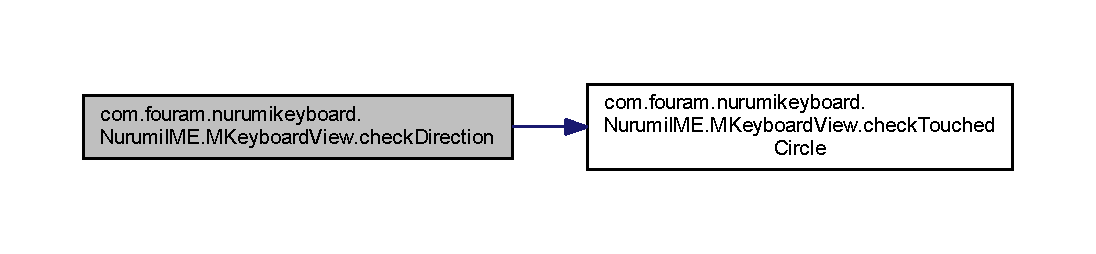
\includegraphics[width=350pt]{classcom_1_1fouram_1_1nurumikeyboard_1_1_nurumi_i_m_e_1_1_m_keyboard_view_aa548466053ead7d81890a197df4e0665_cgraph}
\end{center}
\end{figure}




Here is the caller graph for this function\+:
\nopagebreak
\begin{figure}[H]
\begin{center}
\leavevmode
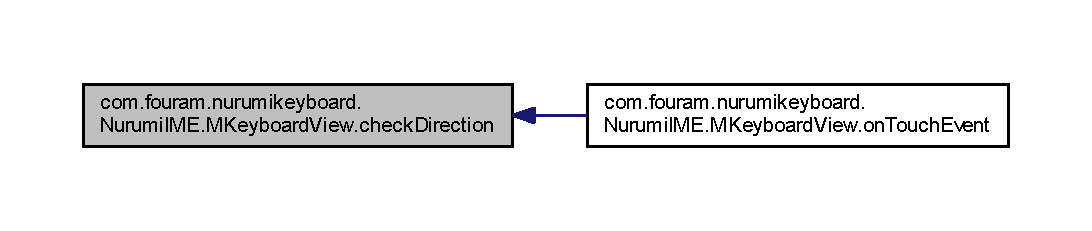
\includegraphics[width=350pt]{classcom_1_1fouram_1_1nurumikeyboard_1_1_nurumi_i_m_e_1_1_m_keyboard_view_aa548466053ead7d81890a197df4e0665_icgraph}
\end{center}
\end{figure}


\hypertarget{classcom_1_1fouram_1_1nurumikeyboard_1_1_nurumi_i_m_e_1_1_m_keyboard_view_ad7701634206a8ad8fb6ad5bc72fc39d1}{}\index{com\+::fouram\+::nurumikeyboard\+::\+Nurumi\+I\+M\+E\+::\+M\+Keyboard\+View@{com\+::fouram\+::nurumikeyboard\+::\+Nurumi\+I\+M\+E\+::\+M\+Keyboard\+View}!check\+Touched\+Circle@{check\+Touched\+Circle}}
\index{check\+Touched\+Circle@{check\+Touched\+Circle}!com\+::fouram\+::nurumikeyboard\+::\+Nurumi\+I\+M\+E\+::\+M\+Keyboard\+View@{com\+::fouram\+::nurumikeyboard\+::\+Nurumi\+I\+M\+E\+::\+M\+Keyboard\+View}}
\subsubsection[{check\+Touched\+Circle}]{\setlength{\rightskip}{0pt plus 5cm}com.\+fouram.\+nurumikeyboard.\+Nurumi\+I\+M\+E.\+M\+Keyboard\+View.\+check\+Touched\+Circle (
\begin{DoxyParamCaption}
\item[{int}]{x, }
\item[{int}]{y}
\end{DoxyParamCaption}
)}\label{classcom_1_1fouram_1_1nurumikeyboard_1_1_nurumi_i_m_e_1_1_m_keyboard_view_ad7701634206a8ad8fb6ad5bc72fc39d1}


Function information \+: Find touched circle. 

\begin{DoxyRemark}{Remarks}

\begin{DoxyItemize}
\item Description \+: This method will check which circle is touched 
\end{DoxyItemize}
\end{DoxyRemark}

\begin{DoxyParams}{Parameters}
{\em x} & x grid of touched point \\
\hline
{\em y} & y grid of touched point \\
\hline
\end{DoxyParams}
\begin{DoxyReturn}{Returns}
Returns touched circle number. If any of circle is touched, return -\/1.
\end{DoxyReturn}

\begin{DoxyCode}
\textcolor{comment}{// core code}
\end{DoxyCode}
 

Definition at line 485 of file M\+Keyboard\+View.\+java.


\begin{DoxyCode}
486     \{       
487         \textcolor{keywordtype}{int} index=0;
488         \textcolor{keywordflow}{for}(PointF spt : \hyperlink{classcom_1_1fouram_1_1nurumikeyboard_1_1_nurumi_i_m_e_1_1_m_keyboard_view_aff948c186aac098473fed848c94fc086}{startPtArr})
489         \{
490             index++;
491             \textcolor{keywordflow}{if}( (Math.abs((\textcolor{keywordtype}{int})spt.x - x) < 180) && (Math.abs((\textcolor{keywordtype}{int})spt.y - y) < 140) )
492                 \textcolor{keywordflow}{return} index;
493         \}
494         \textcolor{keywordflow}{return} -1;
495     \} \textcolor{comment}{// checkTouchedCircle fin}
\end{DoxyCode}


Here is the caller graph for this function\+:
\nopagebreak
\begin{figure}[H]
\begin{center}
\leavevmode
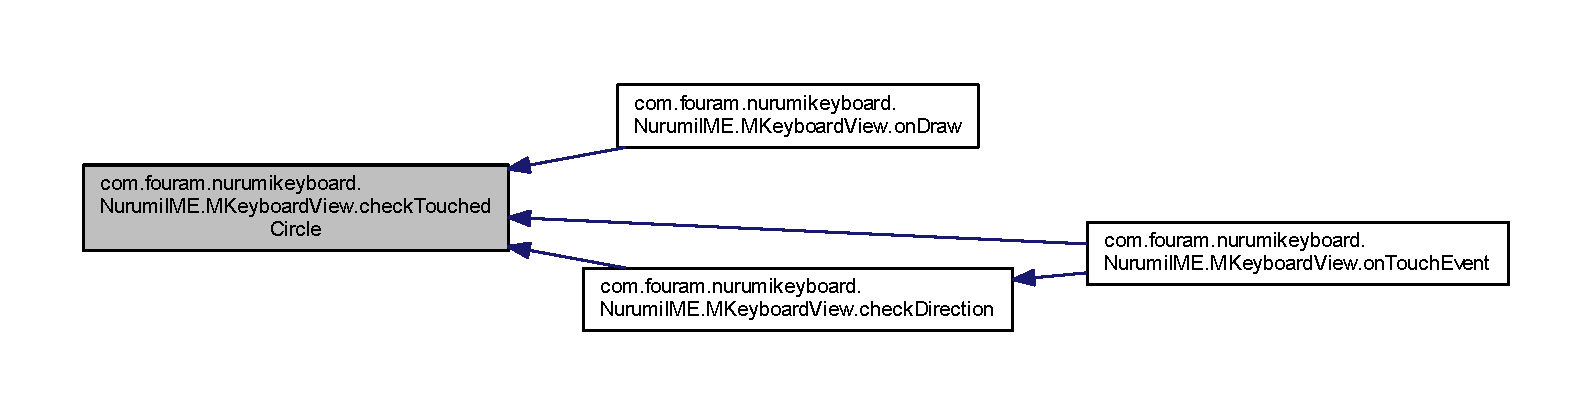
\includegraphics[width=350pt]{classcom_1_1fouram_1_1nurumikeyboard_1_1_nurumi_i_m_e_1_1_m_keyboard_view_ad7701634206a8ad8fb6ad5bc72fc39d1_icgraph}
\end{center}
\end{figure}


\hypertarget{classcom_1_1fouram_1_1nurumikeyboard_1_1_nurumi_i_m_e_1_1_m_keyboard_view_a536f8d1527df8c5013dc66d253ac5dae}{}\index{com\+::fouram\+::nurumikeyboard\+::\+Nurumi\+I\+M\+E\+::\+M\+Keyboard\+View@{com\+::fouram\+::nurumikeyboard\+::\+Nurumi\+I\+M\+E\+::\+M\+Keyboard\+View}!initialize@{initialize}}
\index{initialize@{initialize}!com\+::fouram\+::nurumikeyboard\+::\+Nurumi\+I\+M\+E\+::\+M\+Keyboard\+View@{com\+::fouram\+::nurumikeyboard\+::\+Nurumi\+I\+M\+E\+::\+M\+Keyboard\+View}}
\subsubsection[{initialize}]{\setlength{\rightskip}{0pt plus 5cm}com.\+fouram.\+nurumikeyboard.\+Nurumi\+I\+M\+E.\+M\+Keyboard\+View.\+initialize (
\begin{DoxyParamCaption}
{}
\end{DoxyParamCaption}
)}\label{classcom_1_1fouram_1_1nurumikeyboard_1_1_nurumi_i_m_e_1_1_m_keyboard_view_a536f8d1527df8c5013dc66d253ac5dae}


Function information \+: Initialize function. 

\begin{DoxyRemark}{Remarks}

\begin{DoxyItemize}
\item Description \+: Initialize all variables and lists
\end{DoxyItemize}
\end{DoxyRemark}

\begin{DoxyCode}
\textcolor{comment}{// core code}
\end{DoxyCode}
 

Definition at line 170 of file M\+Keyboard\+View.\+java.


\begin{DoxyCode}
171     \{
172         \hyperlink{classcom_1_1fouram_1_1nurumikeyboard_1_1_nurumi_i_m_e_1_1_m_keyboard_view_a113cc5cd53707a1d2df822c487dcbe8c}{pnt} = \textcolor{keyword}{new} Paint();
173         \hyperlink{classcom_1_1fouram_1_1nurumikeyboard_1_1_nurumi_i_m_e_1_1_m_keyboard_view_af2f59861ed61c6357020e1350be33a5a}{numFingers} = \hyperlink{classcom_1_1fouram_1_1nurumikeyboard_1_1_nurumi_i_m_e_1_1_m_keyboard_view_a61263eb41eed8667a83505e8771c5b23}{FIVE\_FINGERS};
174         \hyperlink{classcom_1_1fouram_1_1nurumikeyboard_1_1_nurumi_i_m_e_1_1_m_keyboard_view_a92db4315e015e0c892d2c324557c599c}{outerCircleSize} = \hyperlink{classcom_1_1fouram_1_1nurumikeyboard_1_1_nurumi_i_m_e_1_1_m_keyboard_view_aabab90ddcaeedf63348d892614c9d168}{OUTER\_CIRCLE\_SIZE};
175         \hyperlink{classcom_1_1fouram_1_1nurumikeyboard_1_1_nurumi_i_m_e_1_1_m_keyboard_view_aa8664e099a4f809a3abf8cdae1c4c393}{innerCircleSize} = \hyperlink{classcom_1_1fouram_1_1nurumikeyboard_1_1_nurumi_i_m_e_1_1_m_keyboard_view_af7119aa21410f68aa856612add4d464c}{INNER\_CIRCLE\_SIZE};
176         
177         \hyperlink{classcom_1_1fouram_1_1nurumikeyboard_1_1_nurumi_i_m_e_1_1_m_keyboard_view_ace13bdd1bb9cdcc07b7c4f6345d51670}{startFlag} = \textcolor{keyword}{false};
178         \hyperlink{classcom_1_1fouram_1_1nurumikeyboard_1_1_nurumi_i_m_e_1_1_m_keyboard_view_a13bdd74ac521ef4655cd139c647de466}{start} = \textcolor{keyword}{false};
179         \hyperlink{classcom_1_1fouram_1_1nurumikeyboard_1_1_nurumi_i_m_e_1_1_m_keyboard_view_a0ac7b4552f63165d0447bbe12a55b813}{motionStartFlag} = \textcolor{keyword}{false};
180         \hyperlink{classcom_1_1fouram_1_1nurumikeyboard_1_1_nurumi_i_m_e_1_1_m_keyboard_view_a33b834fb352211295449e26a9f495807}{motion} = \textcolor{keyword}{new} \textcolor{keywordtype}{int}[\hyperlink{classcom_1_1fouram_1_1nurumikeyboard_1_1_nurumi_i_m_e_1_1_m_keyboard_view_af2f59861ed61c6357020e1350be33a5a}{numFingers}];
181         \hyperlink{classcom_1_1fouram_1_1nurumikeyboard_1_1_nurumi_i_m_e_1_1_m_keyboard_view_a087c107ffdad9ad25e5d28bd003a15c9}{circleAvailable} = \textcolor{keyword}{new} \textcolor{keywordtype}{boolean}[\hyperlink{classcom_1_1fouram_1_1nurumikeyboard_1_1_nurumi_i_m_e_1_1_m_keyboard_view_af2f59861ed61c6357020e1350be33a5a}{numFingers}];
182         \textcolor{keywordflow}{for}(\textcolor{keywordtype}{int} i=0; i<\hyperlink{classcom_1_1fouram_1_1nurumikeyboard_1_1_nurumi_i_m_e_1_1_m_keyboard_view_af2f59861ed61c6357020e1350be33a5a}{numFingers}; i++)
183             \hyperlink{classcom_1_1fouram_1_1nurumikeyboard_1_1_nurumi_i_m_e_1_1_m_keyboard_view_a087c107ffdad9ad25e5d28bd003a15c9}{circleAvailable}[i] = \textcolor{keyword}{true};
184         
185         \hyperlink{classcom_1_1fouram_1_1nurumikeyboard_1_1_nurumi_i_m_e_1_1_m_keyboard_view_a759f646f0682c75387d7a0d8cd3d8cbf}{plp} = \textcolor{keyword}{new} LinkedList<PtIdLinkedWithPtIndex>();
186         \hyperlink{classcom_1_1fouram_1_1nurumikeyboard_1_1_nurumi_i_m_e_1_1_m_keyboard_view_adba837582df67530dd4a9d93fc1825a9}{clp} = \textcolor{keyword}{new} ArrayList<CircleLinkedWithPtId>();
187         
188         \hyperlink{classcom_1_1fouram_1_1nurumikeyboard_1_1_nurumi_i_m_e_1_1_m_keyboard_view_aff948c186aac098473fed848c94fc086}{startPtArr} = \textcolor{keyword}{new} ArrayList<PointF>();
189         \hyperlink{classcom_1_1fouram_1_1nurumikeyboard_1_1_nurumi_i_m_e_1_1_m_keyboard_view_ac7da84e25f4d6414da9023da4a8d3ffa}{oldPtArr} = \textcolor{keyword}{new} ArrayList<PointF>();
190         \hyperlink{classcom_1_1fouram_1_1nurumikeyboard_1_1_nurumi_i_m_e_1_1_m_keyboard_view_a803bbeb52f830df78ab726874a9e7e17}{ptArr} = \textcolor{keyword}{new} ArrayList<PointF>();
191         
192         \hyperlink{classcom_1_1fouram_1_1nurumikeyboard_1_1_nurumi_i_m_e_1_1_m_keyboard_view_a759f646f0682c75387d7a0d8cd3d8cbf}{plp}.clear();
193         clp.clear();
194         
195         startPtArr.clear();
196         oldPtArr.clear();
197         ptArr.clear();
198     \}
\end{DoxyCode}


Here is the caller graph for this function\+:
\nopagebreak
\begin{figure}[H]
\begin{center}
\leavevmode
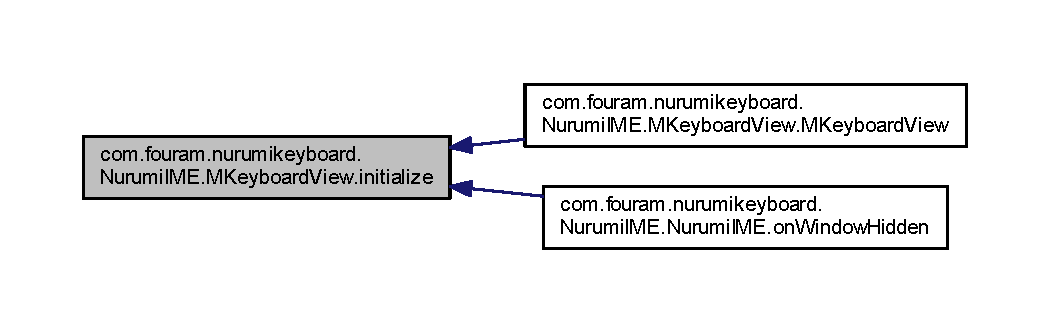
\includegraphics[width=350pt]{classcom_1_1fouram_1_1nurumikeyboard_1_1_nurumi_i_m_e_1_1_m_keyboard_view_a536f8d1527df8c5013dc66d253ac5dae_icgraph}
\end{center}
\end{figure}


\hypertarget{classcom_1_1fouram_1_1nurumikeyboard_1_1_nurumi_i_m_e_1_1_m_keyboard_view_a657f24f9888d141266179c6dc971103f}{}\index{com\+::fouram\+::nurumikeyboard\+::\+Nurumi\+I\+M\+E\+::\+M\+Keyboard\+View@{com\+::fouram\+::nurumikeyboard\+::\+Nurumi\+I\+M\+E\+::\+M\+Keyboard\+View}!motion\+Check@{motion\+Check}}
\index{motion\+Check@{motion\+Check}!com\+::fouram\+::nurumikeyboard\+::\+Nurumi\+I\+M\+E\+::\+M\+Keyboard\+View@{com\+::fouram\+::nurumikeyboard\+::\+Nurumi\+I\+M\+E\+::\+M\+Keyboard\+View}}
\subsubsection[{motion\+Check}]{\setlength{\rightskip}{0pt plus 5cm}com.\+fouram.\+nurumikeyboard.\+Nurumi\+I\+M\+E.\+M\+Keyboard\+View.\+motion\+Check (
\begin{DoxyParamCaption}
{}
\end{DoxyParamCaption}
)}\label{classcom_1_1fouram_1_1nurumikeyboard_1_1_nurumi_i_m_e_1_1_m_keyboard_view_a657f24f9888d141266179c6dc971103f}


Function information \+: Motion checking method. 

\begin{DoxyRemark}{Remarks}

\begin{DoxyItemize}
\item Description \+: In A\+C\+T\+I\+O\+N\+\_\+\+U\+P motion event, this method will be called.~\newline
 Checks motion array and check motion of each pointer.~\newline

\begin{DoxyCode}
\textcolor{comment}{// core code}
\end{DoxyCode}
 
\end{DoxyItemize}
\end{DoxyRemark}


Definition at line 422 of file M\+Keyboard\+View.\+java.


\begin{DoxyCode}
423     \{
424         String command = \textcolor{stringliteral}{""};
425         \textcolor{keywordflow}{for}(\textcolor{keywordtype}{int} i=0; i<\hyperlink{classcom_1_1fouram_1_1nurumikeyboard_1_1_nurumi_i_m_e_1_1_m_keyboard_view_af2f59861ed61c6357020e1350be33a5a}{numFingers}; i++)
426         \{
427             \textcolor{keywordflow}{if}(\hyperlink{classcom_1_1fouram_1_1nurumikeyboard_1_1_nurumi_i_m_e_1_1_m_keyboard_view_a33b834fb352211295449e26a9f495807}{motion}[i] != -1)
428             \{
429                 \textcolor{keywordflow}{switch}(\hyperlink{classcom_1_1fouram_1_1nurumikeyboard_1_1_nurumi_i_m_e_1_1_m_keyboard_view_a33b834fb352211295449e26a9f495807}{motion}[i])
430                 \{
431                     \textcolor{keywordflow}{case} \hyperlink{classcom_1_1fouram_1_1nurumikeyboard_1_1_nurumi_i_m_e_1_1_m_keyboard_view_ab3af4b0b8e75ae26bc33534c1736c701}{DIRECTION\_DOT} :
432                     \{
433                         Log.d(\textcolor{stringliteral}{"UP"}, \textcolor{stringliteral}{"circleIndex : "} + (i+1) + \textcolor{stringliteral}{"| Dir) DOT"});
434                         command += \textcolor{stringliteral}{"circleIndex : "} + (i+1) + \textcolor{stringliteral}{"| Dir) DOT\(\backslash\)n"};
435                         \textcolor{keywordflow}{break};
436                     \}
437                     \textcolor{keywordflow}{case} \hyperlink{classcom_1_1fouram_1_1nurumikeyboard_1_1_nurumi_i_m_e_1_1_m_keyboard_view_a720a8b5a9553d6b9bc0fcb94bf387eaa}{DIRECTION\_UP} :
438                     \{
439                         Log.d(\textcolor{stringliteral}{"UP"}, \textcolor{stringliteral}{"circleIndex : "} + (i+1) + \textcolor{stringliteral}{"| Dir) UP"});
440                         command += \textcolor{stringliteral}{"circleIndex : "} + (i+1) + \textcolor{stringliteral}{"| Dir) UP\(\backslash\)n"};
441                         \textcolor{keywordflow}{break};
442                     \}
443                     \textcolor{keywordflow}{case} \hyperlink{classcom_1_1fouram_1_1nurumikeyboard_1_1_nurumi_i_m_e_1_1_m_keyboard_view_a244ae46f473dfa5074d64a5af1e90ecf}{DIRECTION\_DOWN} :
444                     \{
445                         Log.d(\textcolor{stringliteral}{"UP"}, \textcolor{stringliteral}{"circleIndex : "} + (i+1) + \textcolor{stringliteral}{"| Dir) DOWN"});
446                         command += \textcolor{stringliteral}{"circleIndex : "} + (i+1) + \textcolor{stringliteral}{"| Dir) DOWN\(\backslash\)n"};
447                         \textcolor{keywordflow}{break};
448                     \}
449                     \textcolor{keywordflow}{case} \hyperlink{classcom_1_1fouram_1_1nurumikeyboard_1_1_nurumi_i_m_e_1_1_m_keyboard_view_ad72ab456e489e8c3e860bfa1d094c057}{DIRECTION\_LEFT} :
450                     \{
451                         Log.d(\textcolor{stringliteral}{"UP"}, \textcolor{stringliteral}{"circleIndex : "} + (i+1) + \textcolor{stringliteral}{"| Dir) LEFT"});
452                         command += \textcolor{stringliteral}{"circleIndex : "} + (i+1) + \textcolor{stringliteral}{"| Dir) LEFT\(\backslash\)n"};
453                         \textcolor{keywordflow}{break};
454                     \}
455                     \textcolor{keywordflow}{case} \hyperlink{classcom_1_1fouram_1_1nurumikeyboard_1_1_nurumi_i_m_e_1_1_m_keyboard_view_a94f48baa64fed71b4f1f316958ba2a3e}{DIRECTION\_RIGHT} :
456                     \{
457                         Log.d(\textcolor{stringliteral}{"UP"}, \textcolor{stringliteral}{"circleIndex : "} + (i+1) + \textcolor{stringliteral}{"| Dir) RIGHT"});
458                         command += \textcolor{stringliteral}{"circleIndex : "} + (i+1) + \textcolor{stringliteral}{"| Dir) RIGHT\(\backslash\)n"};
459                     \}
460                 \}\textcolor{comment}{//switch end}
461             \}\textcolor{comment}{//motion check if end}
462         \}\textcolor{comment}{//motion check for end}
463         Log.d(\textcolor{stringliteral}{"Motion End"}, \textcolor{stringliteral}{"------------------------------"});
464         \textcolor{keywordflow}{if}(!command.equals(\textcolor{stringliteral}{""}))
465         \{
466             Toast.makeText(ctx, command, android.widget.Toast.LENGTH\_SHORT).show();
467             \textcolor{comment}{/* key event will be here. */}
468         \}
469         command = \textcolor{stringliteral}{""};
470     \}
\end{DoxyCode}


Here is the caller graph for this function\+:
\nopagebreak
\begin{figure}[H]
\begin{center}
\leavevmode
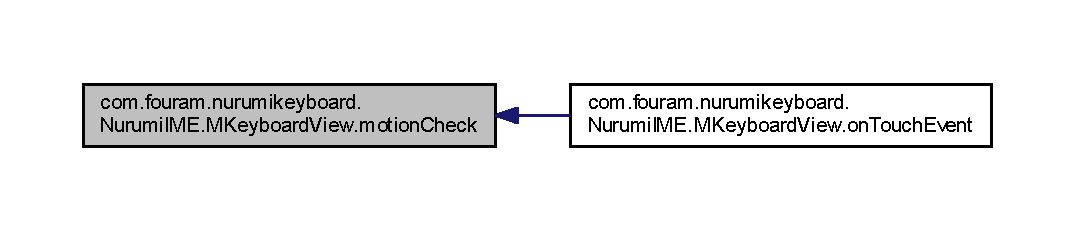
\includegraphics[width=350pt]{classcom_1_1fouram_1_1nurumikeyboard_1_1_nurumi_i_m_e_1_1_m_keyboard_view_a657f24f9888d141266179c6dc971103f_icgraph}
\end{center}
\end{figure}


\hypertarget{classcom_1_1fouram_1_1nurumikeyboard_1_1_nurumi_i_m_e_1_1_m_keyboard_view_a775825f89451ffcdacfbceb7fa201d48}{}\index{com\+::fouram\+::nurumikeyboard\+::\+Nurumi\+I\+M\+E\+::\+M\+Keyboard\+View@{com\+::fouram\+::nurumikeyboard\+::\+Nurumi\+I\+M\+E\+::\+M\+Keyboard\+View}!on\+Draw@{on\+Draw}}
\index{on\+Draw@{on\+Draw}!com\+::fouram\+::nurumikeyboard\+::\+Nurumi\+I\+M\+E\+::\+M\+Keyboard\+View@{com\+::fouram\+::nurumikeyboard\+::\+Nurumi\+I\+M\+E\+::\+M\+Keyboard\+View}}
\subsubsection[{on\+Draw}]{\setlength{\rightskip}{0pt plus 5cm}void com.\+fouram.\+nurumikeyboard.\+Nurumi\+I\+M\+E.\+M\+Keyboard\+View.\+on\+Draw (
\begin{DoxyParamCaption}
\item[{Canvas}]{canvas}
\end{DoxyParamCaption}
)}\label{classcom_1_1fouram_1_1nurumikeyboard_1_1_nurumi_i_m_e_1_1_m_keyboard_view_a775825f89451ffcdacfbceb7fa201d48}


Definition at line 214 of file M\+Keyboard\+View.\+java.


\begin{DoxyCode}
214                                       \{
215         super.onDraw(canvas);
216         canvas.drawColor(Color.TRANSPARENT);
217         
218         \hyperlink{classcom_1_1fouram_1_1nurumikeyboard_1_1_nurumi_i_m_e_1_1_m_keyboard_view_a113cc5cd53707a1d2df822c487dcbe8c}{pnt}.setTextSize(64.0f);
219         
220         \textcolor{comment}{/* standard position */}
221         \textcolor{keywordflow}{if}(\hyperlink{classcom_1_1fouram_1_1nurumikeyboard_1_1_nurumi_i_m_e_1_1_m_keyboard_view_aff948c186aac098473fed848c94fc086}{startPtArr}.isEmpty())
222             \textcolor{keywordflow}{return};
223         \textcolor{keywordtype}{int} index=0;
224         \textcolor{keywordflow}{for}(PointF spt : \hyperlink{classcom_1_1fouram_1_1nurumikeyboard_1_1_nurumi_i_m_e_1_1_m_keyboard_view_aff948c186aac098473fed848c94fc086}{startPtArr})
225         \{
226             index++;
227             \hyperlink{classcom_1_1fouram_1_1nurumikeyboard_1_1_nurumi_i_m_e_1_1_m_keyboard_view_a113cc5cd53707a1d2df822c487dcbe8c}{pnt}.setColor(Color.BLACK);
228             \hyperlink{classcom_1_1fouram_1_1nurumikeyboard_1_1_nurumi_i_m_e_1_1_m_keyboard_view_a113cc5cd53707a1d2df822c487dcbe8c}{pnt}.setStyle(Paint.Style.STROKE);
229             \hyperlink{classcom_1_1fouram_1_1nurumikeyboard_1_1_nurumi_i_m_e_1_1_m_keyboard_view_a113cc5cd53707a1d2df822c487dcbe8c}{pnt}.setStrokeWidth(1);
230             canvas.drawCircle(spt.x,spt.y, \hyperlink{classcom_1_1fouram_1_1nurumikeyboard_1_1_nurumi_i_m_e_1_1_m_keyboard_view_a92db4315e015e0c892d2c324557c599c}{outerCircleSize}, \hyperlink{classcom_1_1fouram_1_1nurumikeyboard_1_1_nurumi_i_m_e_1_1_m_keyboard_view_a113cc5cd53707a1d2df822c487dcbe8c}{pnt});
231 
232             \hyperlink{classcom_1_1fouram_1_1nurumikeyboard_1_1_nurumi_i_m_e_1_1_m_keyboard_view_a113cc5cd53707a1d2df822c487dcbe8c}{pnt}.setStyle(Paint.Style.FILL);
233             canvas.drawText(String.valueOf(index),spt.x,spt.y-((int)(
      \hyperlink{classcom_1_1fouram_1_1nurumikeyboard_1_1_nurumi_i_m_e_1_1_m_keyboard_view_a92db4315e015e0c892d2c324557c599c}{outerCircleSize}/0.8)),\hyperlink{classcom_1_1fouram_1_1nurumikeyboard_1_1_nurumi_i_m_e_1_1_m_keyboard_view_a113cc5cd53707a1d2df822c487dcbe8c}{pnt});
234         \}
235         
236         \textcolor{comment}{/* down event position */}
237         \textcolor{keywordflow}{if}(!\hyperlink{classcom_1_1fouram_1_1nurumikeyboard_1_1_nurumi_i_m_e_1_1_m_keyboard_view_ac7da84e25f4d6414da9023da4a8d3ffa}{oldPtArr}.isEmpty())
238         \{
239             \textcolor{keywordflow}{for} (PointF pt : \hyperlink{classcom_1_1fouram_1_1nurumikeyboard_1_1_nurumi_i_m_e_1_1_m_keyboard_view_ac7da84e25f4d6414da9023da4a8d3ffa}{oldPtArr})
240             \{
241                 \textcolor{keywordtype}{int} circleNum = \hyperlink{classcom_1_1fouram_1_1nurumikeyboard_1_1_nurumi_i_m_e_1_1_m_keyboard_view_ad7701634206a8ad8fb6ad5bc72fc39d1}{checkTouchedCircle}((\textcolor{keywordtype}{int})pt.x, (\textcolor{keywordtype}{int})pt.y);
242                 \hyperlink{classcom_1_1fouram_1_1nurumikeyboard_1_1_nurumi_i_m_e_1_1_m_keyboard_view_a113cc5cd53707a1d2df822c487dcbe8c}{pnt}.setStyle(Paint.Style.STROKE);
243                 canvas.drawCircle(pt.x,pt.y, \hyperlink{classcom_1_1fouram_1_1nurumikeyboard_1_1_nurumi_i_m_e_1_1_m_keyboard_view_aa8664e099a4f809a3abf8cdae1c4c393}{innerCircleSize}, \hyperlink{classcom_1_1fouram_1_1nurumikeyboard_1_1_nurumi_i_m_e_1_1_m_keyboard_view_a113cc5cd53707a1d2df822c487dcbe8c}{pnt});
244 
245                 \hyperlink{classcom_1_1fouram_1_1nurumikeyboard_1_1_nurumi_i_m_e_1_1_m_keyboard_view_a113cc5cd53707a1d2df822c487dcbe8c}{pnt}.setStyle(Paint.Style.FILL);
246                 canvas.drawText(String.valueOf(circleNum),pt.x,pt.y-((int)(
      \hyperlink{classcom_1_1fouram_1_1nurumikeyboard_1_1_nurumi_i_m_e_1_1_m_keyboard_view_a92db4315e015e0c892d2c324557c599c}{outerCircleSize}/0.8)),\hyperlink{classcom_1_1fouram_1_1nurumikeyboard_1_1_nurumi_i_m_e_1_1_m_keyboard_view_a113cc5cd53707a1d2df822c487dcbe8c}{pnt});
247             \}
248         \}
249         
250         \textcolor{comment}{/* current finger */}
251         index=0;
252         \textcolor{keywordflow}{if}(!\hyperlink{classcom_1_1fouram_1_1nurumikeyboard_1_1_nurumi_i_m_e_1_1_m_keyboard_view_a803bbeb52f830df78ab726874a9e7e17}{ptArr}.isEmpty() && !\hyperlink{classcom_1_1fouram_1_1nurumikeyboard_1_1_nurumi_i_m_e_1_1_m_keyboard_view_a759f646f0682c75387d7a0d8cd3d8cbf}{plp}.isEmpty() && !\hyperlink{classcom_1_1fouram_1_1nurumikeyboard_1_1_nurumi_i_m_e_1_1_m_keyboard_view_adba837582df67530dd4a9d93fc1825a9}{clp}.isEmpty())
253         \{           
254             \textcolor{keywordflow}{for} (PointF pt : \hyperlink{classcom_1_1fouram_1_1nurumikeyboard_1_1_nurumi_i_m_e_1_1_m_keyboard_view_a803bbeb52f830df78ab726874a9e7e17}{ptArr})
255             \{
256                 \textcolor{keywordtype}{int} pointerId = \hyperlink{classcom_1_1fouram_1_1nurumikeyboard_1_1_nurumi_i_m_e_1_1_m_keyboard_view_a759f646f0682c75387d7a0d8cd3d8cbf}{plp}.get(index++).pointerId;
257                 \textcolor{keywordflow}{if}(pointerId >= \hyperlink{classcom_1_1fouram_1_1nurumikeyboard_1_1_nurumi_i_m_e_1_1_m_keyboard_view_adba837582df67530dd4a9d93fc1825a9}{clp}.size())
258                     \textcolor{keywordflow}{break};                  
259                 \textcolor{keywordtype}{int} circleNum = \hyperlink{classcom_1_1fouram_1_1nurumikeyboard_1_1_nurumi_i_m_e_1_1_m_keyboard_view_adba837582df67530dd4a9d93fc1825a9}{clp}.get(pointerId).circleNum;
260                 
261                 \hyperlink{classcom_1_1fouram_1_1nurumikeyboard_1_1_nurumi_i_m_e_1_1_m_keyboard_view_a113cc5cd53707a1d2df822c487dcbe8c}{pnt}.setStyle(Paint.Style.STROKE);
262                 canvas.drawCircle(pt.x,pt.y, \hyperlink{classcom_1_1fouram_1_1nurumikeyboard_1_1_nurumi_i_m_e_1_1_m_keyboard_view_aa8664e099a4f809a3abf8cdae1c4c393}{innerCircleSize}, \hyperlink{classcom_1_1fouram_1_1nurumikeyboard_1_1_nurumi_i_m_e_1_1_m_keyboard_view_a113cc5cd53707a1d2df822c487dcbe8c}{pnt});
263 
264                 \hyperlink{classcom_1_1fouram_1_1nurumikeyboard_1_1_nurumi_i_m_e_1_1_m_keyboard_view_a113cc5cd53707a1d2df822c487dcbe8c}{pnt}.setStyle(Paint.Style.FILL);
265                 canvas.drawText(String.valueOf(circleNum),pt.x,pt.y-((int)(
      \hyperlink{classcom_1_1fouram_1_1nurumikeyboard_1_1_nurumi_i_m_e_1_1_m_keyboard_view_a92db4315e015e0c892d2c324557c599c}{outerCircleSize}/0.8)),\hyperlink{classcom_1_1fouram_1_1nurumikeyboard_1_1_nurumi_i_m_e_1_1_m_keyboard_view_a113cc5cd53707a1d2df822c487dcbe8c}{pnt});
266             \}
267         \}
268         
269     \} \textcolor{comment}{// onDraw fin}
\end{DoxyCode}


Here is the call graph for this function\+:
\nopagebreak
\begin{figure}[H]
\begin{center}
\leavevmode
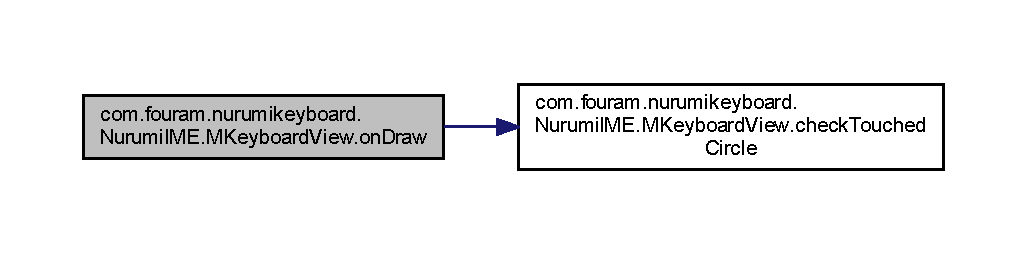
\includegraphics[width=350pt]{classcom_1_1fouram_1_1nurumikeyboard_1_1_nurumi_i_m_e_1_1_m_keyboard_view_a775825f89451ffcdacfbceb7fa201d48_cgraph}
\end{center}
\end{figure}


\hypertarget{classcom_1_1fouram_1_1nurumikeyboard_1_1_nurumi_i_m_e_1_1_m_keyboard_view_a18509488a51daf21c5b16841aaa035c9}{}\index{com\+::fouram\+::nurumikeyboard\+::\+Nurumi\+I\+M\+E\+::\+M\+Keyboard\+View@{com\+::fouram\+::nurumikeyboard\+::\+Nurumi\+I\+M\+E\+::\+M\+Keyboard\+View}!on\+Touch\+Event@{on\+Touch\+Event}}
\index{on\+Touch\+Event@{on\+Touch\+Event}!com\+::fouram\+::nurumikeyboard\+::\+Nurumi\+I\+M\+E\+::\+M\+Keyboard\+View@{com\+::fouram\+::nurumikeyboard\+::\+Nurumi\+I\+M\+E\+::\+M\+Keyboard\+View}}
\subsubsection[{on\+Touch\+Event}]{\setlength{\rightskip}{0pt plus 5cm}com.\+fouram.\+nurumikeyboard.\+Nurumi\+I\+M\+E.\+M\+Keyboard\+View.\+on\+Touch\+Event (
\begin{DoxyParamCaption}
\item[{Motion\+Event}]{e}
\end{DoxyParamCaption}
)}\label{classcom_1_1fouram_1_1nurumikeyboard_1_1_nurumi_i_m_e_1_1_m_keyboard_view_a18509488a51daf21c5b16841aaa035c9}


Function information \+: Touch event method. 

\begin{DoxyRemark}{Remarks}

\begin{DoxyItemize}
\item Description \+: This method will classify motion events.~\newline
 Used Motion\+Event.\+A\+C\+T\+I\+O\+N\+\_\+\+M\+A\+S\+K for recognize A\+C\+T\+I\+O\+N\+\_\+\+P\+O\+I\+N\+T\+E\+R events.~\newline
 A\+C\+T\+I\+O\+N\+\_\+\+D\+O\+W\+N, A\+C\+T\+I\+O\+N\+\_\+\+P\+O\+I\+N\+T\+E\+R\+\_\+\+D\+O\+W\+N, A\+C\+T\+I\+O\+N\+\_\+\+U\+P, A\+C\+T\+I\+O\+N\+\_\+\+P\+O\+I\+N\+T\+E\+R\+\_\+\+U\+P, A\+C\+T\+I\+O\+N\+\_\+\+M\+O\+V\+E, A\+C\+T\+I\+O\+N\+\_\+\+C\+A\+N\+C\+E\+L, and other event(default) will be recognzied. 
\end{DoxyItemize}
\end{DoxyRemark}

\begin{DoxyParams}{Parameters}
{\em e} & A motion event \\
\hline
\end{DoxyParams}
\begin{DoxyReturn}{Returns}
Returns boolean value wether the touch event is valid or not.
\end{DoxyReturn}

\begin{DoxyCode}
\textcolor{comment}{// core code}
\end{DoxyCode}
 

Definition at line 291 of file M\+Keyboard\+View.\+java.


\begin{DoxyCode}
292     \{
293         \textcolor{keywordtype}{int} action = e.getAction() & MotionEvent.ACTION\_MASK;
294         
295         \textcolor{keywordflow}{if}(\hyperlink{classcom_1_1fouram_1_1nurumikeyboard_1_1_nurumi_i_m_e_1_1_m_keyboard_view_a13bdd74ac521ef4655cd139c647de466}{start} == \textcolor{keyword}{false})
296             \textcolor{keywordflow}{return} \hyperlink{classcom_1_1fouram_1_1nurumikeyboard_1_1_nurumi_i_m_e_1_1_m_keyboard_view_a2e05b77b14ceb804926bc33e9e3e88fa}{startMultiTouch}(e);
297         \textcolor{keywordflow}{else}
298         \{               
299             \textcolor{keywordflow}{switch}(action)
300             \{
301                 \textcolor{keywordflow}{case} MotionEvent.ACTION\_DOWN :
302                 \{
303                     \textcolor{keywordflow}{if}( \hyperlink{classcom_1_1fouram_1_1nurumikeyboard_1_1_nurumi_i_m_e_1_1_m_keyboard_view_ad7701634206a8ad8fb6ad5bc72fc39d1}{checkTouchedCircle}((\textcolor{keywordtype}{int})e.getX(), (int)e.getY()) == 
      \hyperlink{classcom_1_1fouram_1_1nurumikeyboard_1_1_nurumi_i_m_e_1_1_m_keyboard_view_a595dcf17ea60a02818d53551cd1dbe4d}{INVALID\_CIRCLE} )
304                         \textcolor{keywordflow}{return} \textcolor{keyword}{false};
305                     \textcolor{keywordflow}{for}(\textcolor{keywordtype}{int} i=0; i<\hyperlink{classcom_1_1fouram_1_1nurumikeyboard_1_1_nurumi_i_m_e_1_1_m_keyboard_view_af2f59861ed61c6357020e1350be33a5a}{numFingers}; i++)
306                         \hyperlink{classcom_1_1fouram_1_1nurumikeyboard_1_1_nurumi_i_m_e_1_1_m_keyboard_view_a33b834fb352211295449e26a9f495807}{motion}[i] = -1;
307                     \hyperlink{classcom_1_1fouram_1_1nurumikeyboard_1_1_nurumi_i_m_e_1_1_m_keyboard_view_a0ac7b4552f63165d0447bbe12a55b813}{motionStartFlag} = \textcolor{keyword}{true};
308                     Log.d(\textcolor{stringliteral}{"Motion Start"}, \textcolor{stringliteral}{"------------------------------"});
309                 \}
310                 \textcolor{keywordflow}{case} MotionEvent.ACTION\_POINTER\_DOWN :
311                 \{
312                     \textcolor{keywordtype}{int} touchCount = e.getPointerCount();
313                     \textcolor{keywordtype}{int} circleNum = \hyperlink{classcom_1_1fouram_1_1nurumikeyboard_1_1_nurumi_i_m_e_1_1_m_keyboard_view_ad7701634206a8ad8fb6ad5bc72fc39d1}{checkTouchedCircle}((\textcolor{keywordtype}{int})e.getX(touchCount-1), (int)e.
      getY(touchCount-1));
314                     \textcolor{keywordflow}{if}(touchCount>numFingers || circleNum == -1 || !
      \hyperlink{classcom_1_1fouram_1_1nurumikeyboard_1_1_nurumi_i_m_e_1_1_m_keyboard_view_a0ac7b4552f63165d0447bbe12a55b813}{motionStartFlag} || !\hyperlink{classcom_1_1fouram_1_1nurumikeyboard_1_1_nurumi_i_m_e_1_1_m_keyboard_view_a087c107ffdad9ad25e5d28bd003a15c9}{circleAvailable}[circleNum-1])
315                     \{
316                         invalidate();
317                         \textcolor{keywordflow}{return} \textcolor{keyword}{true};
318                     \}                       
319                     \hyperlink{classcom_1_1fouram_1_1nurumikeyboard_1_1_nurumi_i_m_e_1_1_m_keyboard_view_a087c107ffdad9ad25e5d28bd003a15c9}{circleAvailable}[circleNum-1] = \textcolor{keyword}{false};
320                     \hyperlink{classcom_1_1fouram_1_1nurumikeyboard_1_1_nurumi_i_m_e_1_1_m_keyboard_view_a33b834fb352211295449e26a9f495807}{motion}[circleNum-1] = \hyperlink{classcom_1_1fouram_1_1nurumikeyboard_1_1_nurumi_i_m_e_1_1_m_keyboard_view_ab3af4b0b8e75ae26bc33534c1736c701}{DIRECTION\_DOT};
321                     
322                     PointF ptf = \textcolor{keyword}{new} PointF();
323                     ptf.x = e.getX(touchCount-1);
324                     ptf.y = e.getY(touchCount-1);
325                     \hyperlink{classcom_1_1fouram_1_1nurumikeyboard_1_1_nurumi_i_m_e_1_1_m_keyboard_view_ac7da84e25f4d6414da9023da4a8d3ffa}{oldPtArr}.add(ptf);
326 
327                     CircleLinkedWithPtId cp = \textcolor{keyword}{new} CircleLinkedWithPtId();
328                     cp.pointerId = e.getPointerId(touchCount-1);
329                     cp.circleNum = circleNum;
330                     \hyperlink{classcom_1_1fouram_1_1nurumikeyboard_1_1_nurumi_i_m_e_1_1_m_keyboard_view_adba837582df67530dd4a9d93fc1825a9}{clp}.add(cp);
331                     
332                     invalidate();
333                     \textcolor{keywordflow}{return} \textcolor{keyword}{true};
334                 \}
335                 
336                 \textcolor{keywordflow}{case} MotionEvent.ACTION\_MOVE :
337                 \{
338                     \hyperlink{classcom_1_1fouram_1_1nurumikeyboard_1_1_nurumi_i_m_e_1_1_m_keyboard_view_a803bbeb52f830df78ab726874a9e7e17}{ptArr}.clear();
339                     \hyperlink{classcom_1_1fouram_1_1nurumikeyboard_1_1_nurumi_i_m_e_1_1_m_keyboard_view_a759f646f0682c75387d7a0d8cd3d8cbf}{plp}.clear();
340                     \textcolor{keywordtype}{int} touchCount = e.getPointerCount();
341                     \textcolor{keywordflow}{if}(touchCount>numFingers)
342                         touchCount = \hyperlink{classcom_1_1fouram_1_1nurumikeyboard_1_1_nurumi_i_m_e_1_1_m_keyboard_view_af2f59861ed61c6357020e1350be33a5a}{numFingers};
343                     \textcolor{keywordflow}{for} (\textcolor{keywordtype}{int} i=0; i<touchCount; i++)
344                     \{
345                         PointF ptf = \textcolor{keyword}{new} PointF();
346                         ptf.x = e.getX(i);
347                         ptf.y = e.getY(i);
348                         \hyperlink{classcom_1_1fouram_1_1nurumikeyboard_1_1_nurumi_i_m_e_1_1_m_keyboard_view_a803bbeb52f830df78ab726874a9e7e17}{ptArr}.add(ptf);
349                         
350                         PtIdLinkedWithPtIndex pp = \textcolor{keyword}{new} PtIdLinkedWithPtIndex();
351                         pp.pointerIndex = i;
352                         pp.pointerId = e.getPointerId(i);
353                         \hyperlink{classcom_1_1fouram_1_1nurumikeyboard_1_1_nurumi_i_m_e_1_1_m_keyboard_view_a759f646f0682c75387d7a0d8cd3d8cbf}{plp}.add(pp);
354                         
355                         \hyperlink{classcom_1_1fouram_1_1nurumikeyboard_1_1_nurumi_i_m_e_1_1_m_keyboard_view_aa548466053ead7d81890a197df4e0665}{checkDirection}(pp, ptf);
356                     \}
357                     invalidate();
358                     \textcolor{keywordflow}{return} \textcolor{keyword}{true};
359                 \}
360                 \textcolor{keywordflow}{case} MotionEvent.ACTION\_POINTER\_UP :
361                 \{
362                     \hyperlink{classcom_1_1fouram_1_1nurumikeyboard_1_1_nurumi_i_m_e_1_1_m_keyboard_view_a0ac7b4552f63165d0447bbe12a55b813}{motionStartFlag} = \textcolor{keyword}{false};
363                     
364                     \textcolor{keywordtype}{int} touchCount = e.getPointerCount();
365                     \textcolor{keywordflow}{if}(touchCount>numFingers)
366                         touchCount = \hyperlink{classcom_1_1fouram_1_1nurumikeyboard_1_1_nurumi_i_m_e_1_1_m_keyboard_view_af2f59861ed61c6357020e1350be33a5a}{numFingers};
367                     \textcolor{keywordflow}{return} \textcolor{keyword}{true};
368                 \}
369                 \textcolor{keywordflow}{case} MotionEvent.ACTION\_UP :
370                 \{
371                     \textcolor{keywordflow}{if}(!\hyperlink{classcom_1_1fouram_1_1nurumikeyboard_1_1_nurumi_i_m_e_1_1_m_keyboard_view_ace13bdd1bb9cdcc07b7c4f6345d51670}{startFlag} && \hyperlink{classcom_1_1fouram_1_1nurumikeyboard_1_1_nurumi_i_m_e_1_1_m_keyboard_view_a13bdd74ac521ef4655cd139c647de466}{start})
372                     \{
373                         \hyperlink{classcom_1_1fouram_1_1nurumikeyboard_1_1_nurumi_i_m_e_1_1_m_keyboard_view_ace13bdd1bb9cdcc07b7c4f6345d51670}{startFlag} = \textcolor{keyword}{true};
374                         \textcolor{keywordflow}{return} \textcolor{keyword}{true};
375                     \}
376                     \textcolor{keywordtype}{int} touchCount = e.getPointerCount();
377                     \textcolor{keywordflow}{if}(touchCount>numFingers)
378                         touchCount = \hyperlink{classcom_1_1fouram_1_1nurumikeyboard_1_1_nurumi_i_m_e_1_1_m_keyboard_view_af2f59861ed61c6357020e1350be33a5a}{numFingers};
379                     \hyperlink{classcom_1_1fouram_1_1nurumikeyboard_1_1_nurumi_i_m_e_1_1_m_keyboard_view_a657f24f9888d141266179c6dc971103f}{motionCheck}();                   
380                     
381                     \textcolor{comment}{/* initialization for next motion */}
382                     \hyperlink{classcom_1_1fouram_1_1nurumikeyboard_1_1_nurumi_i_m_e_1_1_m_keyboard_view_ac7da84e25f4d6414da9023da4a8d3ffa}{oldPtArr}.clear();
383                     \hyperlink{classcom_1_1fouram_1_1nurumikeyboard_1_1_nurumi_i_m_e_1_1_m_keyboard_view_a803bbeb52f830df78ab726874a9e7e17}{ptArr}.clear();
384                     \hyperlink{classcom_1_1fouram_1_1nurumikeyboard_1_1_nurumi_i_m_e_1_1_m_keyboard_view_adba837582df67530dd4a9d93fc1825a9}{clp}.clear();
385                     \hyperlink{classcom_1_1fouram_1_1nurumikeyboard_1_1_nurumi_i_m_e_1_1_m_keyboard_view_a759f646f0682c75387d7a0d8cd3d8cbf}{plp}.clear();
386                     \textcolor{keywordflow}{for}(\textcolor{keywordtype}{int} i=0; i<\hyperlink{classcom_1_1fouram_1_1nurumikeyboard_1_1_nurumi_i_m_e_1_1_m_keyboard_view_af2f59861ed61c6357020e1350be33a5a}{numFingers}; i++)
387                         \hyperlink{classcom_1_1fouram_1_1nurumikeyboard_1_1_nurumi_i_m_e_1_1_m_keyboard_view_a087c107ffdad9ad25e5d28bd003a15c9}{circleAvailable}[i] = \textcolor{keyword}{true};
388                     \hyperlink{classcom_1_1fouram_1_1nurumikeyboard_1_1_nurumi_i_m_e_1_1_m_keyboard_view_a6af440ca9c6043f361e51ead2e95620a}{performClick}();
389                     invalidate();                   
390                     \textcolor{keywordflow}{return} \textcolor{keyword}{true};
391                 \}
392                 \textcolor{keywordflow}{case} MotionEvent.ACTION\_CANCEL :
393                 \{
394                     \hyperlink{classcom_1_1fouram_1_1nurumikeyboard_1_1_nurumi_i_m_e_1_1_m_keyboard_view_ac7da84e25f4d6414da9023da4a8d3ffa}{oldPtArr}.clear();
395                     \hyperlink{classcom_1_1fouram_1_1nurumikeyboard_1_1_nurumi_i_m_e_1_1_m_keyboard_view_a803bbeb52f830df78ab726874a9e7e17}{ptArr}.clear();
396                     \hyperlink{classcom_1_1fouram_1_1nurumikeyboard_1_1_nurumi_i_m_e_1_1_m_keyboard_view_adba837582df67530dd4a9d93fc1825a9}{clp}.clear();
397                     \hyperlink{classcom_1_1fouram_1_1nurumikeyboard_1_1_nurumi_i_m_e_1_1_m_keyboard_view_a759f646f0682c75387d7a0d8cd3d8cbf}{plp}.clear();
398                     \textcolor{keywordflow}{for}(\textcolor{keywordtype}{int} i=0; i<\hyperlink{classcom_1_1fouram_1_1nurumikeyboard_1_1_nurumi_i_m_e_1_1_m_keyboard_view_af2f59861ed61c6357020e1350be33a5a}{numFingers}; i++)
399                         \hyperlink{classcom_1_1fouram_1_1nurumikeyboard_1_1_nurumi_i_m_e_1_1_m_keyboard_view_a087c107ffdad9ad25e5d28bd003a15c9}{circleAvailable}[i] = \textcolor{keyword}{true};
400                     invalidate();
401                     \textcolor{keywordflow}{return} \textcolor{keyword}{false};
402                 \}
403                 \textcolor{keywordflow}{default} :
404                 \{
405                     invalidate();
406                     \textcolor{keywordflow}{return} \textcolor{keyword}{false};
407                 \}       
408             \}
409         \}
410     \} \textcolor{comment}{// onTouchEvent fin}
\end{DoxyCode}


Here is the call graph for this function\+:
\nopagebreak
\begin{figure}[H]
\begin{center}
\leavevmode
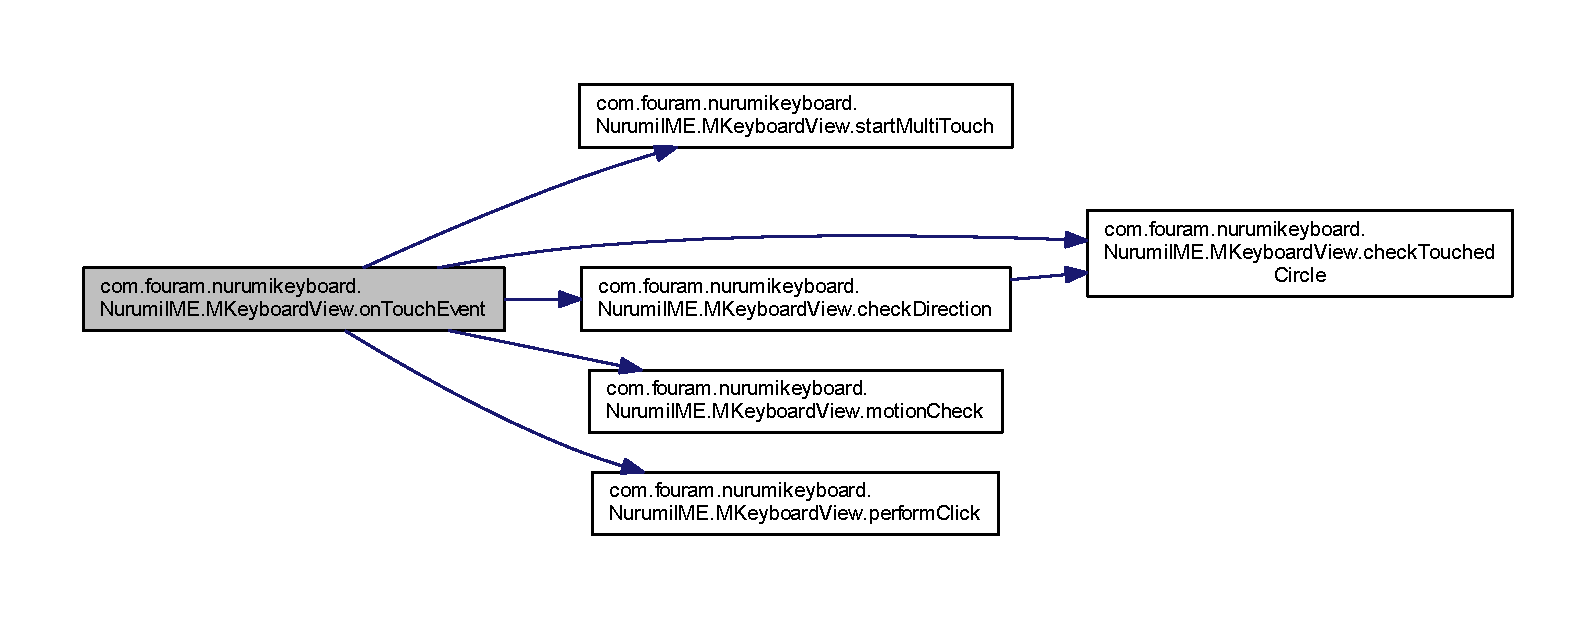
\includegraphics[width=350pt]{classcom_1_1fouram_1_1nurumikeyboard_1_1_nurumi_i_m_e_1_1_m_keyboard_view_a18509488a51daf21c5b16841aaa035c9_cgraph}
\end{center}
\end{figure}


\hypertarget{classcom_1_1fouram_1_1nurumikeyboard_1_1_nurumi_i_m_e_1_1_m_keyboard_view_a6af440ca9c6043f361e51ead2e95620a}{}\index{com\+::fouram\+::nurumikeyboard\+::\+Nurumi\+I\+M\+E\+::\+M\+Keyboard\+View@{com\+::fouram\+::nurumikeyboard\+::\+Nurumi\+I\+M\+E\+::\+M\+Keyboard\+View}!perform\+Click@{perform\+Click}}
\index{perform\+Click@{perform\+Click}!com\+::fouram\+::nurumikeyboard\+::\+Nurumi\+I\+M\+E\+::\+M\+Keyboard\+View@{com\+::fouram\+::nurumikeyboard\+::\+Nurumi\+I\+M\+E\+::\+M\+Keyboard\+View}}
\subsubsection[{perform\+Click}]{\setlength{\rightskip}{0pt plus 5cm}boolean com.\+fouram.\+nurumikeyboard.\+Nurumi\+I\+M\+E.\+M\+Keyboard\+View.\+perform\+Click (
\begin{DoxyParamCaption}
{}
\end{DoxyParamCaption}
)}\label{classcom_1_1fouram_1_1nurumikeyboard_1_1_nurumi_i_m_e_1_1_m_keyboard_view_a6af440ca9c6043f361e51ead2e95620a}


Definition at line 272 of file M\+Keyboard\+View.\+java.


\begin{DoxyCode}
272                                   \{
273         \textcolor{keywordflow}{return} super.performClick();
274     \}
\end{DoxyCode}


Here is the caller graph for this function\+:
\nopagebreak
\begin{figure}[H]
\begin{center}
\leavevmode
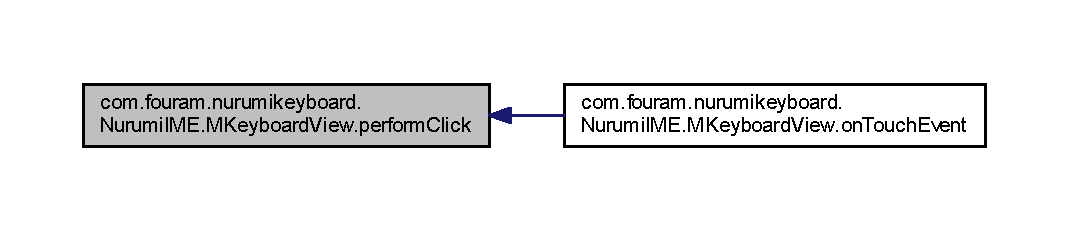
\includegraphics[width=350pt]{classcom_1_1fouram_1_1nurumikeyboard_1_1_nurumi_i_m_e_1_1_m_keyboard_view_a6af440ca9c6043f361e51ead2e95620a_icgraph}
\end{center}
\end{figure}


\hypertarget{classcom_1_1fouram_1_1nurumikeyboard_1_1_nurumi_i_m_e_1_1_m_keyboard_view_a2e05b77b14ceb804926bc33e9e3e88fa}{}\index{com\+::fouram\+::nurumikeyboard\+::\+Nurumi\+I\+M\+E\+::\+M\+Keyboard\+View@{com\+::fouram\+::nurumikeyboard\+::\+Nurumi\+I\+M\+E\+::\+M\+Keyboard\+View}!start\+Multi\+Touch@{start\+Multi\+Touch}}
\index{start\+Multi\+Touch@{start\+Multi\+Touch}!com\+::fouram\+::nurumikeyboard\+::\+Nurumi\+I\+M\+E\+::\+M\+Keyboard\+View@{com\+::fouram\+::nurumikeyboard\+::\+Nurumi\+I\+M\+E\+::\+M\+Keyboard\+View}}
\subsubsection[{start\+Multi\+Touch}]{\setlength{\rightskip}{0pt plus 5cm}com.\+fouram.\+nurumikeyboard.\+Nurumi\+I\+M\+E.\+M\+Keyboard\+View.\+start\+Multi\+Touch (
\begin{DoxyParamCaption}
\item[{Motion\+Event}]{e}
\end{DoxyParamCaption}
)}\label{classcom_1_1fouram_1_1nurumikeyboard_1_1_nurumi_i_m_e_1_1_m_keyboard_view_a2e05b77b14ceb804926bc33e9e3e88fa}


Function information \+: Start multi touch recognition. 

\begin{DoxyRemark}{Remarks}

\begin{DoxyItemize}
\item Description \+: If \textquotesingle{}num\+Fingers\textquotesingle{} of fingers are touched, set \textquotesingle{}start\textquotesingle{} flag true and start multi touch motion recognition.~\newline
 Set \textquotesingle{}num\+Fingers\textquotesingle{} of starting points. 
\end{DoxyItemize}
\end{DoxyRemark}

\begin{DoxyParams}{Parameters}
{\em e} & A motion event \\
\hline
\end{DoxyParams}
\begin{DoxyReturn}{Returns}
Returns the boolean value of motion event is valid or not.
\end{DoxyReturn}

\begin{DoxyCode}
\textcolor{comment}{// core code}
\end{DoxyCode}
 

Definition at line 511 of file M\+Keyboard\+View.\+java.


\begin{DoxyCode}
512     \{
513         \hyperlink{classcom_1_1fouram_1_1nurumikeyboard_1_1_nurumi_i_m_e_1_1_m_keyboard_view_aff948c186aac098473fed848c94fc086}{startPtArr}.clear();
514         \textcolor{keywordflow}{if} ( e.getAction() == MotionEvent.ACTION\_DOWN || e.getAction() == MotionEvent.ACTION\_MOVE )
515         \{
516             \textcolor{keywordtype}{int} touchCount = e.getPointerCount();       
517             \textcolor{keywordflow}{if}(touchCount == \hyperlink{classcom_1_1fouram_1_1nurumikeyboard_1_1_nurumi_i_m_e_1_1_m_keyboard_view_af2f59861ed61c6357020e1350be33a5a}{numFingers})
518             \{
519                 \hyperlink{classcom_1_1fouram_1_1nurumikeyboard_1_1_nurumi_i_m_e_1_1_m_keyboard_view_a13bdd74ac521ef4655cd139c647de466}{start} = \textcolor{keyword}{true};
520                 Log.d(\textcolor{stringliteral}{"start"} , \textcolor{stringliteral}{"start : "} + \hyperlink{classcom_1_1fouram_1_1nurumikeyboard_1_1_nurumi_i_m_e_1_1_m_keyboard_view_a13bdd74ac521ef4655cd139c647de466}{start});
521                 \textcolor{keywordflow}{for} (\textcolor{keywordtype}{int} i=0; i<touchCount; i++)
522                 \{
523                     PointF ptf = \textcolor{keyword}{new} PointF();
524                     ptf.x = e.getX(i);
525                     ptf.y = e.getY(i);
526                     \hyperlink{classcom_1_1fouram_1_1nurumikeyboard_1_1_nurumi_i_m_e_1_1_m_keyboard_view_aff948c186aac098473fed848c94fc086}{startPtArr}.add(ptf);
527                 \}
528                 Collections.sort(\hyperlink{classcom_1_1fouram_1_1nurumikeyboard_1_1_nurumi_i_m_e_1_1_m_keyboard_view_aff948c186aac098473fed848c94fc086}{startPtArr}, comparatorX);
529                 \textcolor{comment}{/*}
530 \textcolor{comment}{                PointF pt1, pt2;}
531 \textcolor{comment}{                pt1 = startPtArr.get(0);}
532 \textcolor{comment}{                pt2 = startPtArr.get(4);}
533 \textcolor{comment}{                if(pt2.x-pt1.x < 800)}
534 \textcolor{comment}{                    Collections.sort(startPtArr, comparatorY);}
535 \textcolor{comment}{                */}
536                 \textcolor{keywordflow}{return} \textcolor{keyword}{true};
537             \}
538             \textcolor{keywordflow}{else} \{\textcolor{keywordflow}{return} \textcolor{keyword}{true};\}
539         \}
540         \textcolor{keywordflow}{else} \{\textcolor{keywordflow}{return} \textcolor{keyword}{false};\}
541     \} \textcolor{comment}{// startMultiTouch fin}
\end{DoxyCode}


Here is the caller graph for this function\+:
\nopagebreak
\begin{figure}[H]
\begin{center}
\leavevmode
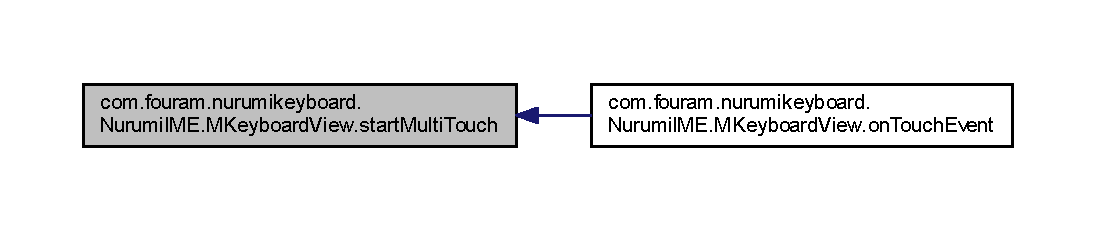
\includegraphics[width=350pt]{classcom_1_1fouram_1_1nurumikeyboard_1_1_nurumi_i_m_e_1_1_m_keyboard_view_a2e05b77b14ceb804926bc33e9e3e88fa_icgraph}
\end{center}
\end{figure}




\subsection{Member Data Documentation}
\hypertarget{classcom_1_1fouram_1_1nurumikeyboard_1_1_nurumi_i_m_e_1_1_m_keyboard_view_a087c107ffdad9ad25e5d28bd003a15c9}{}\index{com\+::fouram\+::nurumikeyboard\+::\+Nurumi\+I\+M\+E\+::\+M\+Keyboard\+View@{com\+::fouram\+::nurumikeyboard\+::\+Nurumi\+I\+M\+E\+::\+M\+Keyboard\+View}!circle\+Available@{circle\+Available}}
\index{circle\+Available@{circle\+Available}!com\+::fouram\+::nurumikeyboard\+::\+Nurumi\+I\+M\+E\+::\+M\+Keyboard\+View@{com\+::fouram\+::nurumikeyboard\+::\+Nurumi\+I\+M\+E\+::\+M\+Keyboard\+View}}
\subsubsection[{circle\+Available}]{\setlength{\rightskip}{0pt plus 5cm}boolean \mbox{[}$\,$\mbox{]} com.\+fouram.\+nurumikeyboard.\+Nurumi\+I\+M\+E.\+M\+Keyboard\+View.\+circle\+Available\hspace{0.3cm}{\ttfamily [private]}}\label{classcom_1_1fouram_1_1nurumikeyboard_1_1_nurumi_i_m_e_1_1_m_keyboard_view_a087c107ffdad9ad25e5d28bd003a15c9}


Definition at line 129 of file M\+Keyboard\+View.\+java.

\hypertarget{classcom_1_1fouram_1_1nurumikeyboard_1_1_nurumi_i_m_e_1_1_m_keyboard_view_adba837582df67530dd4a9d93fc1825a9}{}\index{com\+::fouram\+::nurumikeyboard\+::\+Nurumi\+I\+M\+E\+::\+M\+Keyboard\+View@{com\+::fouram\+::nurumikeyboard\+::\+Nurumi\+I\+M\+E\+::\+M\+Keyboard\+View}!clp@{clp}}
\index{clp@{clp}!com\+::fouram\+::nurumikeyboard\+::\+Nurumi\+I\+M\+E\+::\+M\+Keyboard\+View@{com\+::fouram\+::nurumikeyboard\+::\+Nurumi\+I\+M\+E\+::\+M\+Keyboard\+View}}
\subsubsection[{clp}]{\setlength{\rightskip}{0pt plus 5cm}Array\+List$<${\bf Circle\+Linked\+With\+Pt\+Id}$>$ com.\+fouram.\+nurumikeyboard.\+Nurumi\+I\+M\+E.\+M\+Keyboard\+View.\+clp\hspace{0.3cm}{\ttfamily [private]}}\label{classcom_1_1fouram_1_1nurumikeyboard_1_1_nurumi_i_m_e_1_1_m_keyboard_view_adba837582df67530dd4a9d93fc1825a9}


Definition at line 133 of file M\+Keyboard\+View.\+java.

\hypertarget{classcom_1_1fouram_1_1nurumikeyboard_1_1_nurumi_i_m_e_1_1_m_keyboard_view_ab3af4b0b8e75ae26bc33534c1736c701}{}\index{com\+::fouram\+::nurumikeyboard\+::\+Nurumi\+I\+M\+E\+::\+M\+Keyboard\+View@{com\+::fouram\+::nurumikeyboard\+::\+Nurumi\+I\+M\+E\+::\+M\+Keyboard\+View}!D\+I\+R\+E\+C\+T\+I\+O\+N\+\_\+\+D\+O\+T@{D\+I\+R\+E\+C\+T\+I\+O\+N\+\_\+\+D\+O\+T}}
\index{D\+I\+R\+E\+C\+T\+I\+O\+N\+\_\+\+D\+O\+T@{D\+I\+R\+E\+C\+T\+I\+O\+N\+\_\+\+D\+O\+T}!com\+::fouram\+::nurumikeyboard\+::\+Nurumi\+I\+M\+E\+::\+M\+Keyboard\+View@{com\+::fouram\+::nurumikeyboard\+::\+Nurumi\+I\+M\+E\+::\+M\+Keyboard\+View}}
\subsubsection[{D\+I\+R\+E\+C\+T\+I\+O\+N\+\_\+\+D\+O\+T}]{\setlength{\rightskip}{0pt plus 5cm}final int com.\+fouram.\+nurumikeyboard.\+Nurumi\+I\+M\+E.\+M\+Keyboard\+View.\+D\+I\+R\+E\+C\+T\+I\+O\+N\+\_\+\+D\+O\+T = 0\hspace{0.3cm}{\ttfamily [static]}, {\ttfamily [private]}}\label{classcom_1_1fouram_1_1nurumikeyboard_1_1_nurumi_i_m_e_1_1_m_keyboard_view_ab3af4b0b8e75ae26bc33534c1736c701}


Definition at line 52 of file M\+Keyboard\+View.\+java.

\hypertarget{classcom_1_1fouram_1_1nurumikeyboard_1_1_nurumi_i_m_e_1_1_m_keyboard_view_a244ae46f473dfa5074d64a5af1e90ecf}{}\index{com\+::fouram\+::nurumikeyboard\+::\+Nurumi\+I\+M\+E\+::\+M\+Keyboard\+View@{com\+::fouram\+::nurumikeyboard\+::\+Nurumi\+I\+M\+E\+::\+M\+Keyboard\+View}!D\+I\+R\+E\+C\+T\+I\+O\+N\+\_\+\+D\+O\+W\+N@{D\+I\+R\+E\+C\+T\+I\+O\+N\+\_\+\+D\+O\+W\+N}}
\index{D\+I\+R\+E\+C\+T\+I\+O\+N\+\_\+\+D\+O\+W\+N@{D\+I\+R\+E\+C\+T\+I\+O\+N\+\_\+\+D\+O\+W\+N}!com\+::fouram\+::nurumikeyboard\+::\+Nurumi\+I\+M\+E\+::\+M\+Keyboard\+View@{com\+::fouram\+::nurumikeyboard\+::\+Nurumi\+I\+M\+E\+::\+M\+Keyboard\+View}}
\subsubsection[{D\+I\+R\+E\+C\+T\+I\+O\+N\+\_\+\+D\+O\+W\+N}]{\setlength{\rightskip}{0pt plus 5cm}final int com.\+fouram.\+nurumikeyboard.\+Nurumi\+I\+M\+E.\+M\+Keyboard\+View.\+D\+I\+R\+E\+C\+T\+I\+O\+N\+\_\+\+D\+O\+W\+N = 1\hspace{0.3cm}{\ttfamily [static]}, {\ttfamily [private]}}\label{classcom_1_1fouram_1_1nurumikeyboard_1_1_nurumi_i_m_e_1_1_m_keyboard_view_a244ae46f473dfa5074d64a5af1e90ecf}


Definition at line 53 of file M\+Keyboard\+View.\+java.

\hypertarget{classcom_1_1fouram_1_1nurumikeyboard_1_1_nurumi_i_m_e_1_1_m_keyboard_view_ad72ab456e489e8c3e860bfa1d094c057}{}\index{com\+::fouram\+::nurumikeyboard\+::\+Nurumi\+I\+M\+E\+::\+M\+Keyboard\+View@{com\+::fouram\+::nurumikeyboard\+::\+Nurumi\+I\+M\+E\+::\+M\+Keyboard\+View}!D\+I\+R\+E\+C\+T\+I\+O\+N\+\_\+\+L\+E\+F\+T@{D\+I\+R\+E\+C\+T\+I\+O\+N\+\_\+\+L\+E\+F\+T}}
\index{D\+I\+R\+E\+C\+T\+I\+O\+N\+\_\+\+L\+E\+F\+T@{D\+I\+R\+E\+C\+T\+I\+O\+N\+\_\+\+L\+E\+F\+T}!com\+::fouram\+::nurumikeyboard\+::\+Nurumi\+I\+M\+E\+::\+M\+Keyboard\+View@{com\+::fouram\+::nurumikeyboard\+::\+Nurumi\+I\+M\+E\+::\+M\+Keyboard\+View}}
\subsubsection[{D\+I\+R\+E\+C\+T\+I\+O\+N\+\_\+\+L\+E\+F\+T}]{\setlength{\rightskip}{0pt plus 5cm}final int com.\+fouram.\+nurumikeyboard.\+Nurumi\+I\+M\+E.\+M\+Keyboard\+View.\+D\+I\+R\+E\+C\+T\+I\+O\+N\+\_\+\+L\+E\+F\+T = 2\hspace{0.3cm}{\ttfamily [static]}, {\ttfamily [private]}}\label{classcom_1_1fouram_1_1nurumikeyboard_1_1_nurumi_i_m_e_1_1_m_keyboard_view_ad72ab456e489e8c3e860bfa1d094c057}


Definition at line 54 of file M\+Keyboard\+View.\+java.

\hypertarget{classcom_1_1fouram_1_1nurumikeyboard_1_1_nurumi_i_m_e_1_1_m_keyboard_view_a94f48baa64fed71b4f1f316958ba2a3e}{}\index{com\+::fouram\+::nurumikeyboard\+::\+Nurumi\+I\+M\+E\+::\+M\+Keyboard\+View@{com\+::fouram\+::nurumikeyboard\+::\+Nurumi\+I\+M\+E\+::\+M\+Keyboard\+View}!D\+I\+R\+E\+C\+T\+I\+O\+N\+\_\+\+R\+I\+G\+H\+T@{D\+I\+R\+E\+C\+T\+I\+O\+N\+\_\+\+R\+I\+G\+H\+T}}
\index{D\+I\+R\+E\+C\+T\+I\+O\+N\+\_\+\+R\+I\+G\+H\+T@{D\+I\+R\+E\+C\+T\+I\+O\+N\+\_\+\+R\+I\+G\+H\+T}!com\+::fouram\+::nurumikeyboard\+::\+Nurumi\+I\+M\+E\+::\+M\+Keyboard\+View@{com\+::fouram\+::nurumikeyboard\+::\+Nurumi\+I\+M\+E\+::\+M\+Keyboard\+View}}
\subsubsection[{D\+I\+R\+E\+C\+T\+I\+O\+N\+\_\+\+R\+I\+G\+H\+T}]{\setlength{\rightskip}{0pt plus 5cm}final int com.\+fouram.\+nurumikeyboard.\+Nurumi\+I\+M\+E.\+M\+Keyboard\+View.\+D\+I\+R\+E\+C\+T\+I\+O\+N\+\_\+\+R\+I\+G\+H\+T = 4\hspace{0.3cm}{\ttfamily [static]}, {\ttfamily [private]}}\label{classcom_1_1fouram_1_1nurumikeyboard_1_1_nurumi_i_m_e_1_1_m_keyboard_view_a94f48baa64fed71b4f1f316958ba2a3e}


Definition at line 56 of file M\+Keyboard\+View.\+java.

\hypertarget{classcom_1_1fouram_1_1nurumikeyboard_1_1_nurumi_i_m_e_1_1_m_keyboard_view_a720a8b5a9553d6b9bc0fcb94bf387eaa}{}\index{com\+::fouram\+::nurumikeyboard\+::\+Nurumi\+I\+M\+E\+::\+M\+Keyboard\+View@{com\+::fouram\+::nurumikeyboard\+::\+Nurumi\+I\+M\+E\+::\+M\+Keyboard\+View}!D\+I\+R\+E\+C\+T\+I\+O\+N\+\_\+\+U\+P@{D\+I\+R\+E\+C\+T\+I\+O\+N\+\_\+\+U\+P}}
\index{D\+I\+R\+E\+C\+T\+I\+O\+N\+\_\+\+U\+P@{D\+I\+R\+E\+C\+T\+I\+O\+N\+\_\+\+U\+P}!com\+::fouram\+::nurumikeyboard\+::\+Nurumi\+I\+M\+E\+::\+M\+Keyboard\+View@{com\+::fouram\+::nurumikeyboard\+::\+Nurumi\+I\+M\+E\+::\+M\+Keyboard\+View}}
\subsubsection[{D\+I\+R\+E\+C\+T\+I\+O\+N\+\_\+\+U\+P}]{\setlength{\rightskip}{0pt plus 5cm}final int com.\+fouram.\+nurumikeyboard.\+Nurumi\+I\+M\+E.\+M\+Keyboard\+View.\+D\+I\+R\+E\+C\+T\+I\+O\+N\+\_\+\+U\+P = 3\hspace{0.3cm}{\ttfamily [static]}, {\ttfamily [private]}}\label{classcom_1_1fouram_1_1nurumikeyboard_1_1_nurumi_i_m_e_1_1_m_keyboard_view_a720a8b5a9553d6b9bc0fcb94bf387eaa}


Definition at line 55 of file M\+Keyboard\+View.\+java.

\hypertarget{classcom_1_1fouram_1_1nurumikeyboard_1_1_nurumi_i_m_e_1_1_m_keyboard_view_a61263eb41eed8667a83505e8771c5b23}{}\index{com\+::fouram\+::nurumikeyboard\+::\+Nurumi\+I\+M\+E\+::\+M\+Keyboard\+View@{com\+::fouram\+::nurumikeyboard\+::\+Nurumi\+I\+M\+E\+::\+M\+Keyboard\+View}!F\+I\+V\+E\+\_\+\+F\+I\+N\+G\+E\+R\+S@{F\+I\+V\+E\+\_\+\+F\+I\+N\+G\+E\+R\+S}}
\index{F\+I\+V\+E\+\_\+\+F\+I\+N\+G\+E\+R\+S@{F\+I\+V\+E\+\_\+\+F\+I\+N\+G\+E\+R\+S}!com\+::fouram\+::nurumikeyboard\+::\+Nurumi\+I\+M\+E\+::\+M\+Keyboard\+View@{com\+::fouram\+::nurumikeyboard\+::\+Nurumi\+I\+M\+E\+::\+M\+Keyboard\+View}}
\subsubsection[{F\+I\+V\+E\+\_\+\+F\+I\+N\+G\+E\+R\+S}]{\setlength{\rightskip}{0pt plus 5cm}final int com.\+fouram.\+nurumikeyboard.\+Nurumi\+I\+M\+E.\+M\+Keyboard\+View.\+F\+I\+V\+E\+\_\+\+F\+I\+N\+G\+E\+R\+S = 5\hspace{0.3cm}{\ttfamily [static]}, {\ttfamily [private]}}\label{classcom_1_1fouram_1_1nurumikeyboard_1_1_nurumi_i_m_e_1_1_m_keyboard_view_a61263eb41eed8667a83505e8771c5b23}


Definition at line 58 of file M\+Keyboard\+View.\+java.

\hypertarget{classcom_1_1fouram_1_1nurumikeyboard_1_1_nurumi_i_m_e_1_1_m_keyboard_view_af7119aa21410f68aa856612add4d464c}{}\index{com\+::fouram\+::nurumikeyboard\+::\+Nurumi\+I\+M\+E\+::\+M\+Keyboard\+View@{com\+::fouram\+::nurumikeyboard\+::\+Nurumi\+I\+M\+E\+::\+M\+Keyboard\+View}!I\+N\+N\+E\+R\+\_\+\+C\+I\+R\+C\+L\+E\+\_\+\+S\+I\+Z\+E@{I\+N\+N\+E\+R\+\_\+\+C\+I\+R\+C\+L\+E\+\_\+\+S\+I\+Z\+E}}
\index{I\+N\+N\+E\+R\+\_\+\+C\+I\+R\+C\+L\+E\+\_\+\+S\+I\+Z\+E@{I\+N\+N\+E\+R\+\_\+\+C\+I\+R\+C\+L\+E\+\_\+\+S\+I\+Z\+E}!com\+::fouram\+::nurumikeyboard\+::\+Nurumi\+I\+M\+E\+::\+M\+Keyboard\+View@{com\+::fouram\+::nurumikeyboard\+::\+Nurumi\+I\+M\+E\+::\+M\+Keyboard\+View}}
\subsubsection[{I\+N\+N\+E\+R\+\_\+\+C\+I\+R\+C\+L\+E\+\_\+\+S\+I\+Z\+E}]{\setlength{\rightskip}{0pt plus 5cm}final int com.\+fouram.\+nurumikeyboard.\+Nurumi\+I\+M\+E.\+M\+Keyboard\+View.\+I\+N\+N\+E\+R\+\_\+\+C\+I\+R\+C\+L\+E\+\_\+\+S\+I\+Z\+E = 100\hspace{0.3cm}{\ttfamily [static]}, {\ttfamily [private]}}\label{classcom_1_1fouram_1_1nurumikeyboard_1_1_nurumi_i_m_e_1_1_m_keyboard_view_af7119aa21410f68aa856612add4d464c}


Definition at line 61 of file M\+Keyboard\+View.\+java.

\hypertarget{classcom_1_1fouram_1_1nurumikeyboard_1_1_nurumi_i_m_e_1_1_m_keyboard_view_aa8664e099a4f809a3abf8cdae1c4c393}{}\index{com\+::fouram\+::nurumikeyboard\+::\+Nurumi\+I\+M\+E\+::\+M\+Keyboard\+View@{com\+::fouram\+::nurumikeyboard\+::\+Nurumi\+I\+M\+E\+::\+M\+Keyboard\+View}!inner\+Circle\+Size@{inner\+Circle\+Size}}
\index{inner\+Circle\+Size@{inner\+Circle\+Size}!com\+::fouram\+::nurumikeyboard\+::\+Nurumi\+I\+M\+E\+::\+M\+Keyboard\+View@{com\+::fouram\+::nurumikeyboard\+::\+Nurumi\+I\+M\+E\+::\+M\+Keyboard\+View}}
\subsubsection[{inner\+Circle\+Size}]{\setlength{\rightskip}{0pt plus 5cm}int com.\+fouram.\+nurumikeyboard.\+Nurumi\+I\+M\+E.\+M\+Keyboard\+View.\+inner\+Circle\+Size\hspace{0.3cm}{\ttfamily [private]}}\label{classcom_1_1fouram_1_1nurumikeyboard_1_1_nurumi_i_m_e_1_1_m_keyboard_view_aa8664e099a4f809a3abf8cdae1c4c393}


Definition at line 126 of file M\+Keyboard\+View.\+java.

\hypertarget{classcom_1_1fouram_1_1nurumikeyboard_1_1_nurumi_i_m_e_1_1_m_keyboard_view_a595dcf17ea60a02818d53551cd1dbe4d}{}\index{com\+::fouram\+::nurumikeyboard\+::\+Nurumi\+I\+M\+E\+::\+M\+Keyboard\+View@{com\+::fouram\+::nurumikeyboard\+::\+Nurumi\+I\+M\+E\+::\+M\+Keyboard\+View}!I\+N\+V\+A\+L\+I\+D\+\_\+\+C\+I\+R\+C\+L\+E@{I\+N\+V\+A\+L\+I\+D\+\_\+\+C\+I\+R\+C\+L\+E}}
\index{I\+N\+V\+A\+L\+I\+D\+\_\+\+C\+I\+R\+C\+L\+E@{I\+N\+V\+A\+L\+I\+D\+\_\+\+C\+I\+R\+C\+L\+E}!com\+::fouram\+::nurumikeyboard\+::\+Nurumi\+I\+M\+E\+::\+M\+Keyboard\+View@{com\+::fouram\+::nurumikeyboard\+::\+Nurumi\+I\+M\+E\+::\+M\+Keyboard\+View}}
\subsubsection[{I\+N\+V\+A\+L\+I\+D\+\_\+\+C\+I\+R\+C\+L\+E}]{\setlength{\rightskip}{0pt plus 5cm}final int com.\+fouram.\+nurumikeyboard.\+Nurumi\+I\+M\+E.\+M\+Keyboard\+View.\+I\+N\+V\+A\+L\+I\+D\+\_\+\+C\+I\+R\+C\+L\+E = -\/1\hspace{0.3cm}{\ttfamily [static]}, {\ttfamily [private]}}\label{classcom_1_1fouram_1_1nurumikeyboard_1_1_nurumi_i_m_e_1_1_m_keyboard_view_a595dcf17ea60a02818d53551cd1dbe4d}


Definition at line 50 of file M\+Keyboard\+View.\+java.

\hypertarget{classcom_1_1fouram_1_1nurumikeyboard_1_1_nurumi_i_m_e_1_1_m_keyboard_view_af02d80d6fbd44cae54c67a461858a5cd}{}\index{com\+::fouram\+::nurumikeyboard\+::\+Nurumi\+I\+M\+E\+::\+M\+Keyboard\+View@{com\+::fouram\+::nurumikeyboard\+::\+Nurumi\+I\+M\+E\+::\+M\+Keyboard\+View}!I\+N\+V\+A\+L\+I\+D\+\_\+\+D\+I\+R\+E\+C\+T\+I\+O\+N@{I\+N\+V\+A\+L\+I\+D\+\_\+\+D\+I\+R\+E\+C\+T\+I\+O\+N}}
\index{I\+N\+V\+A\+L\+I\+D\+\_\+\+D\+I\+R\+E\+C\+T\+I\+O\+N@{I\+N\+V\+A\+L\+I\+D\+\_\+\+D\+I\+R\+E\+C\+T\+I\+O\+N}!com\+::fouram\+::nurumikeyboard\+::\+Nurumi\+I\+M\+E\+::\+M\+Keyboard\+View@{com\+::fouram\+::nurumikeyboard\+::\+Nurumi\+I\+M\+E\+::\+M\+Keyboard\+View}}
\subsubsection[{I\+N\+V\+A\+L\+I\+D\+\_\+\+D\+I\+R\+E\+C\+T\+I\+O\+N}]{\setlength{\rightskip}{0pt plus 5cm}final int com.\+fouram.\+nurumikeyboard.\+Nurumi\+I\+M\+E.\+M\+Keyboard\+View.\+I\+N\+V\+A\+L\+I\+D\+\_\+\+D\+I\+R\+E\+C\+T\+I\+O\+N = -\/1\hspace{0.3cm}{\ttfamily [static]}, {\ttfamily [private]}}\label{classcom_1_1fouram_1_1nurumikeyboard_1_1_nurumi_i_m_e_1_1_m_keyboard_view_af02d80d6fbd44cae54c67a461858a5cd}


Definition at line 51 of file M\+Keyboard\+View.\+java.

\hypertarget{classcom_1_1fouram_1_1nurumikeyboard_1_1_nurumi_i_m_e_1_1_m_keyboard_view_a33b834fb352211295449e26a9f495807}{}\index{com\+::fouram\+::nurumikeyboard\+::\+Nurumi\+I\+M\+E\+::\+M\+Keyboard\+View@{com\+::fouram\+::nurumikeyboard\+::\+Nurumi\+I\+M\+E\+::\+M\+Keyboard\+View}!motion@{motion}}
\index{motion@{motion}!com\+::fouram\+::nurumikeyboard\+::\+Nurumi\+I\+M\+E\+::\+M\+Keyboard\+View@{com\+::fouram\+::nurumikeyboard\+::\+Nurumi\+I\+M\+E\+::\+M\+Keyboard\+View}}
\subsubsection[{motion}]{\setlength{\rightskip}{0pt plus 5cm}int \mbox{[}$\,$\mbox{]} com.\+fouram.\+nurumikeyboard.\+Nurumi\+I\+M\+E.\+M\+Keyboard\+View.\+motion\hspace{0.3cm}{\ttfamily [private]}}\label{classcom_1_1fouram_1_1nurumikeyboard_1_1_nurumi_i_m_e_1_1_m_keyboard_view_a33b834fb352211295449e26a9f495807}


Definition at line 128 of file M\+Keyboard\+View.\+java.

\hypertarget{classcom_1_1fouram_1_1nurumikeyboard_1_1_nurumi_i_m_e_1_1_m_keyboard_view_a0ac7b4552f63165d0447bbe12a55b813}{}\index{com\+::fouram\+::nurumikeyboard\+::\+Nurumi\+I\+M\+E\+::\+M\+Keyboard\+View@{com\+::fouram\+::nurumikeyboard\+::\+Nurumi\+I\+M\+E\+::\+M\+Keyboard\+View}!motion\+Start\+Flag@{motion\+Start\+Flag}}
\index{motion\+Start\+Flag@{motion\+Start\+Flag}!com\+::fouram\+::nurumikeyboard\+::\+Nurumi\+I\+M\+E\+::\+M\+Keyboard\+View@{com\+::fouram\+::nurumikeyboard\+::\+Nurumi\+I\+M\+E\+::\+M\+Keyboard\+View}}
\subsubsection[{motion\+Start\+Flag}]{\setlength{\rightskip}{0pt plus 5cm}boolean com.\+fouram.\+nurumikeyboard.\+Nurumi\+I\+M\+E.\+M\+Keyboard\+View.\+motion\+Start\+Flag\hspace{0.3cm}{\ttfamily [private]}}\label{classcom_1_1fouram_1_1nurumikeyboard_1_1_nurumi_i_m_e_1_1_m_keyboard_view_a0ac7b4552f63165d0447bbe12a55b813}


Definition at line 138 of file M\+Keyboard\+View.\+java.

\hypertarget{classcom_1_1fouram_1_1nurumikeyboard_1_1_nurumi_i_m_e_1_1_m_keyboard_view_af2f59861ed61c6357020e1350be33a5a}{}\index{com\+::fouram\+::nurumikeyboard\+::\+Nurumi\+I\+M\+E\+::\+M\+Keyboard\+View@{com\+::fouram\+::nurumikeyboard\+::\+Nurumi\+I\+M\+E\+::\+M\+Keyboard\+View}!num\+Fingers@{num\+Fingers}}
\index{num\+Fingers@{num\+Fingers}!com\+::fouram\+::nurumikeyboard\+::\+Nurumi\+I\+M\+E\+::\+M\+Keyboard\+View@{com\+::fouram\+::nurumikeyboard\+::\+Nurumi\+I\+M\+E\+::\+M\+Keyboard\+View}}
\subsubsection[{num\+Fingers}]{\setlength{\rightskip}{0pt plus 5cm}int com.\+fouram.\+nurumikeyboard.\+Nurumi\+I\+M\+E.\+M\+Keyboard\+View.\+num\+Fingers\hspace{0.3cm}{\ttfamily [private]}}\label{classcom_1_1fouram_1_1nurumikeyboard_1_1_nurumi_i_m_e_1_1_m_keyboard_view_af2f59861ed61c6357020e1350be33a5a}


Definition at line 125 of file M\+Keyboard\+View.\+java.

\hypertarget{classcom_1_1fouram_1_1nurumikeyboard_1_1_nurumi_i_m_e_1_1_m_keyboard_view_ac7da84e25f4d6414da9023da4a8d3ffa}{}\index{com\+::fouram\+::nurumikeyboard\+::\+Nurumi\+I\+M\+E\+::\+M\+Keyboard\+View@{com\+::fouram\+::nurumikeyboard\+::\+Nurumi\+I\+M\+E\+::\+M\+Keyboard\+View}!old\+Pt\+Arr@{old\+Pt\+Arr}}
\index{old\+Pt\+Arr@{old\+Pt\+Arr}!com\+::fouram\+::nurumikeyboard\+::\+Nurumi\+I\+M\+E\+::\+M\+Keyboard\+View@{com\+::fouram\+::nurumikeyboard\+::\+Nurumi\+I\+M\+E\+::\+M\+Keyboard\+View}}
\subsubsection[{old\+Pt\+Arr}]{\setlength{\rightskip}{0pt plus 5cm}Array\+List$<$Point\+F$>$ com.\+fouram.\+nurumikeyboard.\+Nurumi\+I\+M\+E.\+M\+Keyboard\+View.\+old\+Pt\+Arr\hspace{0.3cm}{\ttfamily [private]}}\label{classcom_1_1fouram_1_1nurumikeyboard_1_1_nurumi_i_m_e_1_1_m_keyboard_view_ac7da84e25f4d6414da9023da4a8d3ffa}


Definition at line 135 of file M\+Keyboard\+View.\+java.

\hypertarget{classcom_1_1fouram_1_1nurumikeyboard_1_1_nurumi_i_m_e_1_1_m_keyboard_view_aabab90ddcaeedf63348d892614c9d168}{}\index{com\+::fouram\+::nurumikeyboard\+::\+Nurumi\+I\+M\+E\+::\+M\+Keyboard\+View@{com\+::fouram\+::nurumikeyboard\+::\+Nurumi\+I\+M\+E\+::\+M\+Keyboard\+View}!O\+U\+T\+E\+R\+\_\+\+C\+I\+R\+C\+L\+E\+\_\+\+S\+I\+Z\+E@{O\+U\+T\+E\+R\+\_\+\+C\+I\+R\+C\+L\+E\+\_\+\+S\+I\+Z\+E}}
\index{O\+U\+T\+E\+R\+\_\+\+C\+I\+R\+C\+L\+E\+\_\+\+S\+I\+Z\+E@{O\+U\+T\+E\+R\+\_\+\+C\+I\+R\+C\+L\+E\+\_\+\+S\+I\+Z\+E}!com\+::fouram\+::nurumikeyboard\+::\+Nurumi\+I\+M\+E\+::\+M\+Keyboard\+View@{com\+::fouram\+::nurumikeyboard\+::\+Nurumi\+I\+M\+E\+::\+M\+Keyboard\+View}}
\subsubsection[{O\+U\+T\+E\+R\+\_\+\+C\+I\+R\+C\+L\+E\+\_\+\+S\+I\+Z\+E}]{\setlength{\rightskip}{0pt plus 5cm}final int com.\+fouram.\+nurumikeyboard.\+Nurumi\+I\+M\+E.\+M\+Keyboard\+View.\+O\+U\+T\+E\+R\+\_\+\+C\+I\+R\+C\+L\+E\+\_\+\+S\+I\+Z\+E = 140\hspace{0.3cm}{\ttfamily [static]}, {\ttfamily [private]}}\label{classcom_1_1fouram_1_1nurumikeyboard_1_1_nurumi_i_m_e_1_1_m_keyboard_view_aabab90ddcaeedf63348d892614c9d168}


Definition at line 60 of file M\+Keyboard\+View.\+java.

\hypertarget{classcom_1_1fouram_1_1nurumikeyboard_1_1_nurumi_i_m_e_1_1_m_keyboard_view_a92db4315e015e0c892d2c324557c599c}{}\index{com\+::fouram\+::nurumikeyboard\+::\+Nurumi\+I\+M\+E\+::\+M\+Keyboard\+View@{com\+::fouram\+::nurumikeyboard\+::\+Nurumi\+I\+M\+E\+::\+M\+Keyboard\+View}!outer\+Circle\+Size@{outer\+Circle\+Size}}
\index{outer\+Circle\+Size@{outer\+Circle\+Size}!com\+::fouram\+::nurumikeyboard\+::\+Nurumi\+I\+M\+E\+::\+M\+Keyboard\+View@{com\+::fouram\+::nurumikeyboard\+::\+Nurumi\+I\+M\+E\+::\+M\+Keyboard\+View}}
\subsubsection[{outer\+Circle\+Size}]{\setlength{\rightskip}{0pt plus 5cm}int com.\+fouram.\+nurumikeyboard.\+Nurumi\+I\+M\+E.\+M\+Keyboard\+View.\+outer\+Circle\+Size\hspace{0.3cm}{\ttfamily [private]}}\label{classcom_1_1fouram_1_1nurumikeyboard_1_1_nurumi_i_m_e_1_1_m_keyboard_view_a92db4315e015e0c892d2c324557c599c}


Definition at line 127 of file M\+Keyboard\+View.\+java.

\hypertarget{classcom_1_1fouram_1_1nurumikeyboard_1_1_nurumi_i_m_e_1_1_m_keyboard_view_a759f646f0682c75387d7a0d8cd3d8cbf}{}\index{com\+::fouram\+::nurumikeyboard\+::\+Nurumi\+I\+M\+E\+::\+M\+Keyboard\+View@{com\+::fouram\+::nurumikeyboard\+::\+Nurumi\+I\+M\+E\+::\+M\+Keyboard\+View}!plp@{plp}}
\index{plp@{plp}!com\+::fouram\+::nurumikeyboard\+::\+Nurumi\+I\+M\+E\+::\+M\+Keyboard\+View@{com\+::fouram\+::nurumikeyboard\+::\+Nurumi\+I\+M\+E\+::\+M\+Keyboard\+View}}
\subsubsection[{plp}]{\setlength{\rightskip}{0pt plus 5cm}Linked\+List$<${\bf Pt\+Id\+Linked\+With\+Pt\+Index}$>$ com.\+fouram.\+nurumikeyboard.\+Nurumi\+I\+M\+E.\+M\+Keyboard\+View.\+plp\hspace{0.3cm}{\ttfamily [private]}}\label{classcom_1_1fouram_1_1nurumikeyboard_1_1_nurumi_i_m_e_1_1_m_keyboard_view_a759f646f0682c75387d7a0d8cd3d8cbf}


Definition at line 132 of file M\+Keyboard\+View.\+java.

\hypertarget{classcom_1_1fouram_1_1nurumikeyboard_1_1_nurumi_i_m_e_1_1_m_keyboard_view_a113cc5cd53707a1d2df822c487dcbe8c}{}\index{com\+::fouram\+::nurumikeyboard\+::\+Nurumi\+I\+M\+E\+::\+M\+Keyboard\+View@{com\+::fouram\+::nurumikeyboard\+::\+Nurumi\+I\+M\+E\+::\+M\+Keyboard\+View}!pnt@{pnt}}
\index{pnt@{pnt}!com\+::fouram\+::nurumikeyboard\+::\+Nurumi\+I\+M\+E\+::\+M\+Keyboard\+View@{com\+::fouram\+::nurumikeyboard\+::\+Nurumi\+I\+M\+E\+::\+M\+Keyboard\+View}}
\subsubsection[{pnt}]{\setlength{\rightskip}{0pt plus 5cm}Paint com.\+fouram.\+nurumikeyboard.\+Nurumi\+I\+M\+E.\+M\+Keyboard\+View.\+pnt\hspace{0.3cm}{\ttfamily [private]}}\label{classcom_1_1fouram_1_1nurumikeyboard_1_1_nurumi_i_m_e_1_1_m_keyboard_view_a113cc5cd53707a1d2df822c487dcbe8c}


Definition at line 123 of file M\+Keyboard\+View.\+java.

\hypertarget{classcom_1_1fouram_1_1nurumikeyboard_1_1_nurumi_i_m_e_1_1_m_keyboard_view_a803bbeb52f830df78ab726874a9e7e17}{}\index{com\+::fouram\+::nurumikeyboard\+::\+Nurumi\+I\+M\+E\+::\+M\+Keyboard\+View@{com\+::fouram\+::nurumikeyboard\+::\+Nurumi\+I\+M\+E\+::\+M\+Keyboard\+View}!pt\+Arr@{pt\+Arr}}
\index{pt\+Arr@{pt\+Arr}!com\+::fouram\+::nurumikeyboard\+::\+Nurumi\+I\+M\+E\+::\+M\+Keyboard\+View@{com\+::fouram\+::nurumikeyboard\+::\+Nurumi\+I\+M\+E\+::\+M\+Keyboard\+View}}
\subsubsection[{pt\+Arr}]{\setlength{\rightskip}{0pt plus 5cm}Array\+List$<$Point\+F$>$ com.\+fouram.\+nurumikeyboard.\+Nurumi\+I\+M\+E.\+M\+Keyboard\+View.\+pt\+Arr\hspace{0.3cm}{\ttfamily [private]}}\label{classcom_1_1fouram_1_1nurumikeyboard_1_1_nurumi_i_m_e_1_1_m_keyboard_view_a803bbeb52f830df78ab726874a9e7e17}


Definition at line 136 of file M\+Keyboard\+View.\+java.

\hypertarget{classcom_1_1fouram_1_1nurumikeyboard_1_1_nurumi_i_m_e_1_1_m_keyboard_view_a13bdd74ac521ef4655cd139c647de466}{}\index{com\+::fouram\+::nurumikeyboard\+::\+Nurumi\+I\+M\+E\+::\+M\+Keyboard\+View@{com\+::fouram\+::nurumikeyboard\+::\+Nurumi\+I\+M\+E\+::\+M\+Keyboard\+View}!start@{start}}
\index{start@{start}!com\+::fouram\+::nurumikeyboard\+::\+Nurumi\+I\+M\+E\+::\+M\+Keyboard\+View@{com\+::fouram\+::nurumikeyboard\+::\+Nurumi\+I\+M\+E\+::\+M\+Keyboard\+View}}
\subsubsection[{start}]{\setlength{\rightskip}{0pt plus 5cm}boolean com.\+fouram.\+nurumikeyboard.\+Nurumi\+I\+M\+E.\+M\+Keyboard\+View.\+start\hspace{0.3cm}{\ttfamily [private]}}\label{classcom_1_1fouram_1_1nurumikeyboard_1_1_nurumi_i_m_e_1_1_m_keyboard_view_a13bdd74ac521ef4655cd139c647de466}


Definition at line 139 of file M\+Keyboard\+View.\+java.

\hypertarget{classcom_1_1fouram_1_1nurumikeyboard_1_1_nurumi_i_m_e_1_1_m_keyboard_view_ace13bdd1bb9cdcc07b7c4f6345d51670}{}\index{com\+::fouram\+::nurumikeyboard\+::\+Nurumi\+I\+M\+E\+::\+M\+Keyboard\+View@{com\+::fouram\+::nurumikeyboard\+::\+Nurumi\+I\+M\+E\+::\+M\+Keyboard\+View}!start\+Flag@{start\+Flag}}
\index{start\+Flag@{start\+Flag}!com\+::fouram\+::nurumikeyboard\+::\+Nurumi\+I\+M\+E\+::\+M\+Keyboard\+View@{com\+::fouram\+::nurumikeyboard\+::\+Nurumi\+I\+M\+E\+::\+M\+Keyboard\+View}}
\subsubsection[{start\+Flag}]{\setlength{\rightskip}{0pt plus 5cm}boolean com.\+fouram.\+nurumikeyboard.\+Nurumi\+I\+M\+E.\+M\+Keyboard\+View.\+start\+Flag\hspace{0.3cm}{\ttfamily [private]}}\label{classcom_1_1fouram_1_1nurumikeyboard_1_1_nurumi_i_m_e_1_1_m_keyboard_view_ace13bdd1bb9cdcc07b7c4f6345d51670}


Definition at line 140 of file M\+Keyboard\+View.\+java.

\hypertarget{classcom_1_1fouram_1_1nurumikeyboard_1_1_nurumi_i_m_e_1_1_m_keyboard_view_aff948c186aac098473fed848c94fc086}{}\index{com\+::fouram\+::nurumikeyboard\+::\+Nurumi\+I\+M\+E\+::\+M\+Keyboard\+View@{com\+::fouram\+::nurumikeyboard\+::\+Nurumi\+I\+M\+E\+::\+M\+Keyboard\+View}!start\+Pt\+Arr@{start\+Pt\+Arr}}
\index{start\+Pt\+Arr@{start\+Pt\+Arr}!com\+::fouram\+::nurumikeyboard\+::\+Nurumi\+I\+M\+E\+::\+M\+Keyboard\+View@{com\+::fouram\+::nurumikeyboard\+::\+Nurumi\+I\+M\+E\+::\+M\+Keyboard\+View}}
\subsubsection[{start\+Pt\+Arr}]{\setlength{\rightskip}{0pt plus 5cm}Array\+List$<$Point\+F$>$ com.\+fouram.\+nurumikeyboard.\+Nurumi\+I\+M\+E.\+M\+Keyboard\+View.\+start\+Pt\+Arr\hspace{0.3cm}{\ttfamily [private]}}\label{classcom_1_1fouram_1_1nurumikeyboard_1_1_nurumi_i_m_e_1_1_m_keyboard_view_aff948c186aac098473fed848c94fc086}


Definition at line 134 of file M\+Keyboard\+View.\+java.

\hypertarget{classcom_1_1fouram_1_1nurumikeyboard_1_1_nurumi_i_m_e_1_1_m_keyboard_view_a6e09544be36903fcc2395fecb6fd3dae}{}\index{com\+::fouram\+::nurumikeyboard\+::\+Nurumi\+I\+M\+E\+::\+M\+Keyboard\+View@{com\+::fouram\+::nurumikeyboard\+::\+Nurumi\+I\+M\+E\+::\+M\+Keyboard\+View}!S\+W\+I\+P\+E\+\_\+\+M\+I\+N\+\_\+\+D\+I\+S\+T\+A\+N\+C\+E@{S\+W\+I\+P\+E\+\_\+\+M\+I\+N\+\_\+\+D\+I\+S\+T\+A\+N\+C\+E}}
\index{S\+W\+I\+P\+E\+\_\+\+M\+I\+N\+\_\+\+D\+I\+S\+T\+A\+N\+C\+E@{S\+W\+I\+P\+E\+\_\+\+M\+I\+N\+\_\+\+D\+I\+S\+T\+A\+N\+C\+E}!com\+::fouram\+::nurumikeyboard\+::\+Nurumi\+I\+M\+E\+::\+M\+Keyboard\+View@{com\+::fouram\+::nurumikeyboard\+::\+Nurumi\+I\+M\+E\+::\+M\+Keyboard\+View}}
\subsubsection[{S\+W\+I\+P\+E\+\_\+\+M\+I\+N\+\_\+\+D\+I\+S\+T\+A\+N\+C\+E}]{\setlength{\rightskip}{0pt plus 5cm}final int com.\+fouram.\+nurumikeyboard.\+Nurumi\+I\+M\+E.\+M\+Keyboard\+View.\+S\+W\+I\+P\+E\+\_\+\+M\+I\+N\+\_\+\+D\+I\+S\+T\+A\+N\+C\+E = 140\hspace{0.3cm}{\ttfamily [static]}, {\ttfamily [private]}}\label{classcom_1_1fouram_1_1nurumikeyboard_1_1_nurumi_i_m_e_1_1_m_keyboard_view_a6e09544be36903fcc2395fecb6fd3dae}


Definition at line 57 of file M\+Keyboard\+View.\+java.

\hypertarget{classcom_1_1fouram_1_1nurumikeyboard_1_1_nurumi_i_m_e_1_1_m_keyboard_view_aa3081bef03a1aa0af4b6ec3496b041cb}{}\index{com\+::fouram\+::nurumikeyboard\+::\+Nurumi\+I\+M\+E\+::\+M\+Keyboard\+View@{com\+::fouram\+::nurumikeyboard\+::\+Nurumi\+I\+M\+E\+::\+M\+Keyboard\+View}!T\+E\+N\+\_\+\+F\+I\+N\+G\+E\+R\+S@{T\+E\+N\+\_\+\+F\+I\+N\+G\+E\+R\+S}}
\index{T\+E\+N\+\_\+\+F\+I\+N\+G\+E\+R\+S@{T\+E\+N\+\_\+\+F\+I\+N\+G\+E\+R\+S}!com\+::fouram\+::nurumikeyboard\+::\+Nurumi\+I\+M\+E\+::\+M\+Keyboard\+View@{com\+::fouram\+::nurumikeyboard\+::\+Nurumi\+I\+M\+E\+::\+M\+Keyboard\+View}}
\subsubsection[{T\+E\+N\+\_\+\+F\+I\+N\+G\+E\+R\+S}]{\setlength{\rightskip}{0pt plus 5cm}final int com.\+fouram.\+nurumikeyboard.\+Nurumi\+I\+M\+E.\+M\+Keyboard\+View.\+T\+E\+N\+\_\+\+F\+I\+N\+G\+E\+R\+S = 10\hspace{0.3cm}{\ttfamily [static]}, {\ttfamily [private]}}\label{classcom_1_1fouram_1_1nurumikeyboard_1_1_nurumi_i_m_e_1_1_m_keyboard_view_aa3081bef03a1aa0af4b6ec3496b041cb}


Definition at line 59 of file M\+Keyboard\+View.\+java.



The documentation for this class was generated from the following file\+:\begin{DoxyCompactItemize}
\item 
src/com/fouram/nurumikeyboard/\+Nurumi\+I\+M\+E/\hyperlink{_m_keyboard_view_8java}{M\+Keyboard\+View.\+java}\end{DoxyCompactItemize}

\hypertarget{classcom_1_1fouram_1_1nurumikeyboard_1_1_nurumi_i_m_e_1_1_nurumi_i_m_e}{}\section{com.\+fouram.\+nurumikeyboard.\+Nurumi\+I\+M\+E.\+Nurumi\+I\+M\+E Class Reference}
\label{classcom_1_1fouram_1_1nurumikeyboard_1_1_nurumi_i_m_e_1_1_nurumi_i_m_e}\index{com.\+fouram.\+nurumikeyboard.\+Nurumi\+I\+M\+E.\+Nurumi\+I\+M\+E@{com.\+fouram.\+nurumikeyboard.\+Nurumi\+I\+M\+E.\+Nurumi\+I\+M\+E}}


Inheritance diagram for com.\+fouram.\+nurumikeyboard.\+Nurumi\+I\+M\+E.\+Nurumi\+I\+M\+E\+:
\nopagebreak
\begin{figure}[H]
\begin{center}
\leavevmode
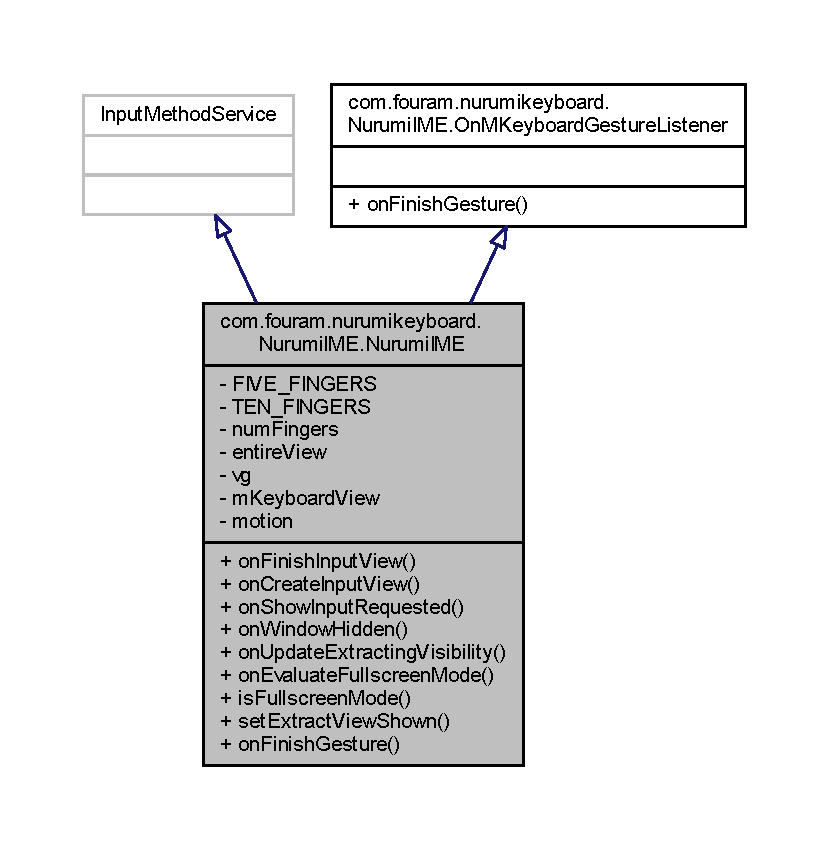
\includegraphics[width=350pt]{classcom_1_1fouram_1_1nurumikeyboard_1_1_nurumi_i_m_e_1_1_nurumi_i_m_e__inherit__graph}
\end{center}
\end{figure}


Collaboration diagram for com.\+fouram.\+nurumikeyboard.\+Nurumi\+I\+M\+E.\+Nurumi\+I\+M\+E\+:
\nopagebreak
\begin{figure}[H]
\begin{center}
\leavevmode
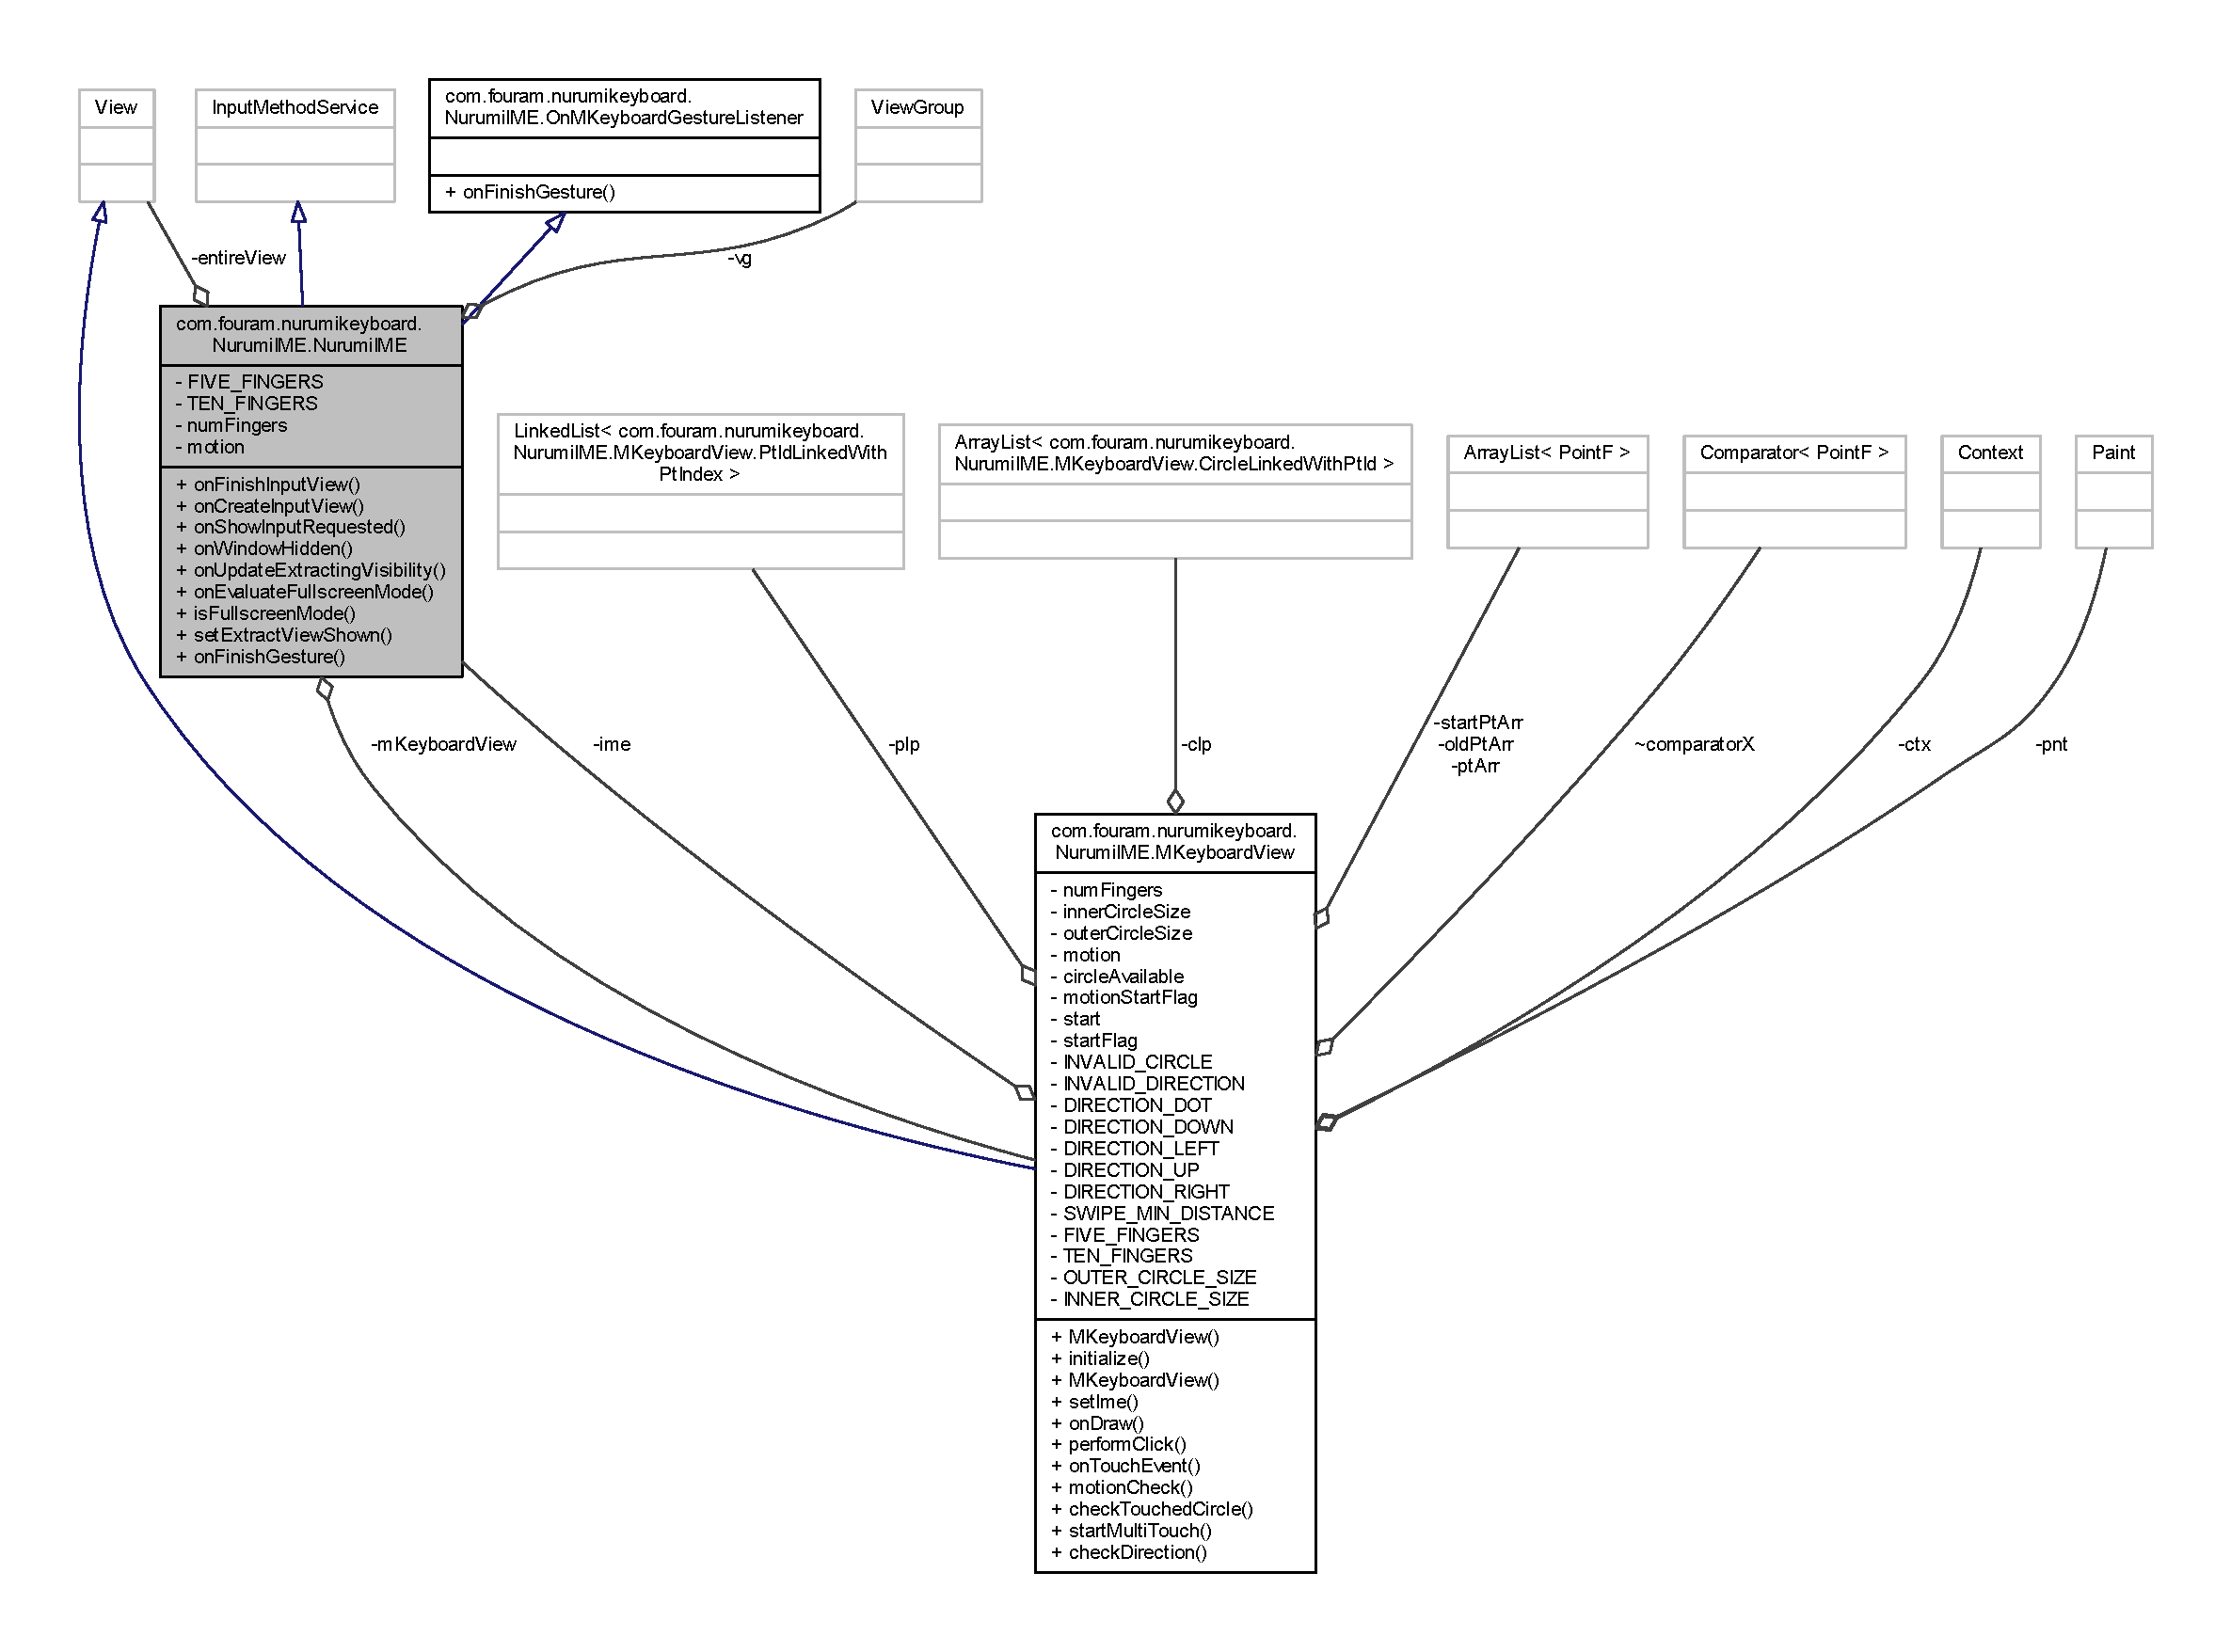
\includegraphics[width=350pt]{classcom_1_1fouram_1_1nurumikeyboard_1_1_nurumi_i_m_e_1_1_nurumi_i_m_e__coll__graph}
\end{center}
\end{figure}
\subsection*{Public Member Functions}
\begin{DoxyCompactItemize}
\item 
void \hyperlink{classcom_1_1fouram_1_1nurumikeyboard_1_1_nurumi_i_m_e_1_1_nurumi_i_m_e_a83c202c960e717ed80dd20c47e760a6c}{on\+Finish\+Input\+View} (boolean finishing\+Input)
\item 
View \hyperlink{classcom_1_1fouram_1_1nurumikeyboard_1_1_nurumi_i_m_e_1_1_nurumi_i_m_e_a2cc9e540f1ef205df73a02b38842f2cf}{on\+Create\+Input\+View} ()
\item 
boolean \hyperlink{classcom_1_1fouram_1_1nurumikeyboard_1_1_nurumi_i_m_e_1_1_nurumi_i_m_e_a187ecc78f108f4f394d63609503315bb}{on\+Show\+Input\+Requested} (int flags, boolean config\+Change)
\item 
void \hyperlink{classcom_1_1fouram_1_1nurumikeyboard_1_1_nurumi_i_m_e_1_1_nurumi_i_m_e_a5917567be1a7c4f177968eb9cb130992}{on\+Window\+Hidden} ()
\item 
void \hyperlink{classcom_1_1fouram_1_1nurumikeyboard_1_1_nurumi_i_m_e_1_1_nurumi_i_m_e_a402ef1ca87efa5c183805ec36e249f5c}{on\+Update\+Extracting\+Visibility} (Editor\+Info ei)
\item 
boolean \hyperlink{classcom_1_1fouram_1_1nurumikeyboard_1_1_nurumi_i_m_e_1_1_nurumi_i_m_e_a8d8939dd9ba019a8ba3536f5529e105e}{on\+Evaluate\+Fullscreen\+Mode} ()
\item 
boolean \hyperlink{classcom_1_1fouram_1_1nurumikeyboard_1_1_nurumi_i_m_e_1_1_nurumi_i_m_e_a7b278c1ebec576db4897dccc7b6b34da}{is\+Fullscreen\+Mode} ()
\item 
void \hyperlink{classcom_1_1fouram_1_1nurumikeyboard_1_1_nurumi_i_m_e_1_1_nurumi_i_m_e_ab2bcb5ce607676ca73f5a64b6b087973}{set\+Extract\+View\+Shown} (boolean shown)
\item 
void \hyperlink{classcom_1_1fouram_1_1nurumikeyboard_1_1_nurumi_i_m_e_1_1_nurumi_i_m_e_a539ed018248c5459a89e102ea4c8d5c5}{on\+Finish\+Gesture} (int\mbox{[}$\,$\mbox{]} \hyperlink{classcom_1_1fouram_1_1nurumikeyboard_1_1_nurumi_i_m_e_1_1_nurumi_i_m_e_ac73ce0e0f969277597c8907855393ea8}{motion})
\end{DoxyCompactItemize}
\subsection*{Private Attributes}
\begin{DoxyCompactItemize}
\item 
final int \hyperlink{classcom_1_1fouram_1_1nurumikeyboard_1_1_nurumi_i_m_e_1_1_nurumi_i_m_e_a9b39dd4573a5446f50b56ae0f0beba4d}{F\+I\+V\+E\+\_\+\+F\+I\+N\+G\+E\+R\+S} = 5
\item 
final int \hyperlink{classcom_1_1fouram_1_1nurumikeyboard_1_1_nurumi_i_m_e_1_1_nurumi_i_m_e_afcdaac68a2da0f716da9b2ea582ea2ad}{T\+E\+N\+\_\+\+F\+I\+N\+G\+E\+R\+S} = 10
\item 
int \hyperlink{classcom_1_1fouram_1_1nurumikeyboard_1_1_nurumi_i_m_e_1_1_nurumi_i_m_e_a8da73863a9fc74d17aa828c3d6d7bf6b}{num\+Fingers}
\item 
View \hyperlink{classcom_1_1fouram_1_1nurumikeyboard_1_1_nurumi_i_m_e_1_1_nurumi_i_m_e_adf766bc5635fcf0dd670402d172e45ba}{entire\+View}
\item 
View\+Group \hyperlink{classcom_1_1fouram_1_1nurumikeyboard_1_1_nurumi_i_m_e_1_1_nurumi_i_m_e_addc58b240728adb839c40fa65e1b89bb}{vg}
\item 
\hyperlink{classcom_1_1fouram_1_1nurumikeyboard_1_1_nurumi_i_m_e_1_1_m_keyboard_view}{M\+Keyboard\+View} \hyperlink{classcom_1_1fouram_1_1nurumikeyboard_1_1_nurumi_i_m_e_1_1_nurumi_i_m_e_a357ffb1d95223caceb27332fecdf4d5c}{m\+Keyboard\+View}
\item 
int\mbox{[}$\,$\mbox{]} \hyperlink{classcom_1_1fouram_1_1nurumikeyboard_1_1_nurumi_i_m_e_1_1_nurumi_i_m_e_ac73ce0e0f969277597c8907855393ea8}{motion}
\end{DoxyCompactItemize}


\subsection{Detailed Description}
\hyperlink{namespacecom_1_1fouram_1_1nurumikeyboard_1_1_nurumi_i_m_e}{com.\+fouram.\+nurumikeyboard.\+Nurumi\+I\+M\+E} ~\newline
 �� \hyperlink{_nurumi_i_m_e_8java}{Nurumi\+I\+M\+E.\+java} \hypertarget{classcom_1_1fouram_1_1nurumikeyboard_1_1_nurumi_i_m_e_1_1_m_keyboard_view_1_1_pt_id_linked_with_pt_index_Class}{}\subsection{information}\label{classcom_1_1fouram_1_1nurumikeyboard_1_1_nurumi_i_m_e_1_1_m_keyboard_view_1_1_pt_id_linked_with_pt_index_Class}
\begin{TabularC}{2}
\hline
\rowcolor{lightgray}\PBS\centering {\bf Item }&{\bf Contents  }\\\cline{1-2}
\PBS\centering Company &4\+:00 A.\+M \\\cline{1-2}
\PBS\centering Author &Park, Hyung Soon \\\cline{1-2}
\PBS\centering Date &2015. 3. 26 \\\cline{1-2}
\end{TabularC}
\hypertarget{classcom_1_1fouram_1_1nurumikeyboard_1_1_nurumi_i_m_e_1_1_m_keyboard_view_1_1_pt_id_linked_with_pt_index_Description}{}\subsection{Description}\label{classcom_1_1fouram_1_1nurumikeyboard_1_1_nurumi_i_m_e_1_1_m_keyboard_view_1_1_pt_id_linked_with_pt_index_Description}

\begin{DoxyItemize}
\item Prototype of gesture based keyboard.
\end{DoxyItemize}

\hyperlink{namespacecom_1_1fouram_1_1nurumikeyboard_1_1_nurumi_i_m_e}{com.\+fouram.\+nurumikeyboard.\+Nurumi\+I\+M\+E} ~\newline
 �� \hyperlink{_nurumi_i_m_e_8java}{Nurumi\+I\+M\+E.\+java} \hypertarget{classcom_1_1fouram_1_1nurumikeyboard_1_1_nurumi_i_m_e_1_1_m_keyboard_view_1_1_pt_id_linked_with_pt_index_Class}{}\subsection{information}\label{classcom_1_1fouram_1_1nurumikeyboard_1_1_nurumi_i_m_e_1_1_m_keyboard_view_1_1_pt_id_linked_with_pt_index_Class}
\begin{TabularC}{2}
\hline
\rowcolor{lightgray}\PBS\centering {\bf Item }&{\bf Contents  }\\\cline{1-2}
\PBS\centering Company &4\+:00 A.\+M. \\\cline{1-2}
\PBS\centering Author &Park, Hyung Soon \\\cline{1-2}
\PBS\centering Date &2015. 3. 26. \\\cline{1-2}
\end{TabularC}
\hypertarget{classcom_1_1fouram_1_1nurumikeyboard_1_1_nurumi_i_m_e_1_1_m_keyboard_view_1_1_pt_id_linked_with_pt_index_Description}{}\subsection{Description}\label{classcom_1_1fouram_1_1nurumikeyboard_1_1_nurumi_i_m_e_1_1_m_keyboard_view_1_1_pt_id_linked_with_pt_index_Description}

\begin{DoxyItemize}
\item Input method service class.~\newline

\item This class makes user to replace keyboard.~\newline

\end{DoxyItemize}

Definition at line 41 of file Nurumi\+I\+M\+E.\+java.



\subsection{Member Function Documentation}
\hypertarget{classcom_1_1fouram_1_1nurumikeyboard_1_1_nurumi_i_m_e_1_1_nurumi_i_m_e_a7b278c1ebec576db4897dccc7b6b34da}{}\index{com\+::fouram\+::nurumikeyboard\+::\+Nurumi\+I\+M\+E\+::\+Nurumi\+I\+M\+E@{com\+::fouram\+::nurumikeyboard\+::\+Nurumi\+I\+M\+E\+::\+Nurumi\+I\+M\+E}!is\+Fullscreen\+Mode@{is\+Fullscreen\+Mode}}
\index{is\+Fullscreen\+Mode@{is\+Fullscreen\+Mode}!com\+::fouram\+::nurumikeyboard\+::\+Nurumi\+I\+M\+E\+::\+Nurumi\+I\+M\+E@{com\+::fouram\+::nurumikeyboard\+::\+Nurumi\+I\+M\+E\+::\+Nurumi\+I\+M\+E}}
\subsubsection[{is\+Fullscreen\+Mode}]{\setlength{\rightskip}{0pt plus 5cm}boolean com.\+fouram.\+nurumikeyboard.\+Nurumi\+I\+M\+E.\+Nurumi\+I\+M\+E.\+is\+Fullscreen\+Mode (
\begin{DoxyParamCaption}
{}
\end{DoxyParamCaption}
)}\label{classcom_1_1fouram_1_1nurumikeyboard_1_1_nurumi_i_m_e_1_1_nurumi_i_m_e_a7b278c1ebec576db4897dccc7b6b34da}


Definition at line 111 of file Nurumi\+I\+M\+E.\+java.


\begin{DoxyCode}
111                                       \{
112         \textcolor{keywordflow}{return} \textcolor{keyword}{true};
113     \}
\end{DoxyCode}
\hypertarget{classcom_1_1fouram_1_1nurumikeyboard_1_1_nurumi_i_m_e_1_1_nurumi_i_m_e_a2cc9e540f1ef205df73a02b38842f2cf}{}\index{com\+::fouram\+::nurumikeyboard\+::\+Nurumi\+I\+M\+E\+::\+Nurumi\+I\+M\+E@{com\+::fouram\+::nurumikeyboard\+::\+Nurumi\+I\+M\+E\+::\+Nurumi\+I\+M\+E}!on\+Create\+Input\+View@{on\+Create\+Input\+View}}
\index{on\+Create\+Input\+View@{on\+Create\+Input\+View}!com\+::fouram\+::nurumikeyboard\+::\+Nurumi\+I\+M\+E\+::\+Nurumi\+I\+M\+E@{com\+::fouram\+::nurumikeyboard\+::\+Nurumi\+I\+M\+E\+::\+Nurumi\+I\+M\+E}}
\subsubsection[{on\+Create\+Input\+View}]{\setlength{\rightskip}{0pt plus 5cm}View com.\+fouram.\+nurumikeyboard.\+Nurumi\+I\+M\+E.\+Nurumi\+I\+M\+E.\+on\+Create\+Input\+View (
\begin{DoxyParamCaption}
{}
\end{DoxyParamCaption}
)}\label{classcom_1_1fouram_1_1nurumikeyboard_1_1_nurumi_i_m_e_1_1_nurumi_i_m_e_a2cc9e540f1ef205df73a02b38842f2cf}


Definition at line 67 of file Nurumi\+I\+M\+E.\+java.


\begin{DoxyCode}
67                                     \{
68         \textcolor{keywordtype}{int} layoutId = R.layout.mkeyboardlayout;
69         \hyperlink{classcom_1_1fouram_1_1nurumikeyboard_1_1_nurumi_i_m_e_1_1_nurumi_i_m_e_adf766bc5635fcf0dd670402d172e45ba}{entireView} = (View)getLayoutInflater().inflate(layoutId, null);
70         \hyperlink{classcom_1_1fouram_1_1nurumikeyboard_1_1_nurumi_i_m_e_1_1_nurumi_i_m_e_addc58b240728adb839c40fa65e1b89bb}{vg} = (ViewGroup) \hyperlink{classcom_1_1fouram_1_1nurumikeyboard_1_1_nurumi_i_m_e_1_1_nurumi_i_m_e_adf766bc5635fcf0dd670402d172e45ba}{entireView};
71         \hyperlink{classcom_1_1fouram_1_1nurumikeyboard_1_1_nurumi_i_m_e_1_1_nurumi_i_m_e_a357ffb1d95223caceb27332fecdf4d5c}{mKeyboardView} = (MKeyboardView) \hyperlink{classcom_1_1fouram_1_1nurumikeyboard_1_1_nurumi_i_m_e_1_1_nurumi_i_m_e_addc58b240728adb839c40fa65e1b89bb}{vg}.findViewById(R.id.MKeyboardView);
72         \hyperlink{classcom_1_1fouram_1_1nurumikeyboard_1_1_nurumi_i_m_e_1_1_nurumi_i_m_e_a357ffb1d95223caceb27332fecdf4d5c}{mKeyboardView}.\hyperlink{classcom_1_1fouram_1_1nurumikeyboard_1_1_nurumi_i_m_e_1_1_m_keyboard_view_a879697fa9b15b251c012e1a6e688acd7}{setIme}(\textcolor{keyword}{this});
73         
74         \hyperlink{classcom_1_1fouram_1_1nurumikeyboard_1_1_nurumi_i_m_e_1_1_nurumi_i_m_e_a8da73863a9fc74d17aa828c3d6d7bf6b}{numFingers} = \hyperlink{classcom_1_1fouram_1_1nurumikeyboard_1_1_nurumi_i_m_e_1_1_nurumi_i_m_e_a9b39dd4573a5446f50b56ae0f0beba4d}{FIVE\_FINGERS};
75         \hyperlink{classcom_1_1fouram_1_1nurumikeyboard_1_1_nurumi_i_m_e_1_1_nurumi_i_m_e_ac73ce0e0f969277597c8907855393ea8}{motion} = \textcolor{keyword}{new} \textcolor{keywordtype}{int}[\hyperlink{classcom_1_1fouram_1_1nurumikeyboard_1_1_nurumi_i_m_e_1_1_nurumi_i_m_e_a8da73863a9fc74d17aa828c3d6d7bf6b}{numFingers}];
76         
77         \textcolor{keywordflow}{return} \hyperlink{classcom_1_1fouram_1_1nurumikeyboard_1_1_nurumi_i_m_e_1_1_nurumi_i_m_e_adf766bc5635fcf0dd670402d172e45ba}{entireView};
78     \}
\end{DoxyCode}


Here is the call graph for this function\+:
\nopagebreak
\begin{figure}[H]
\begin{center}
\leavevmode
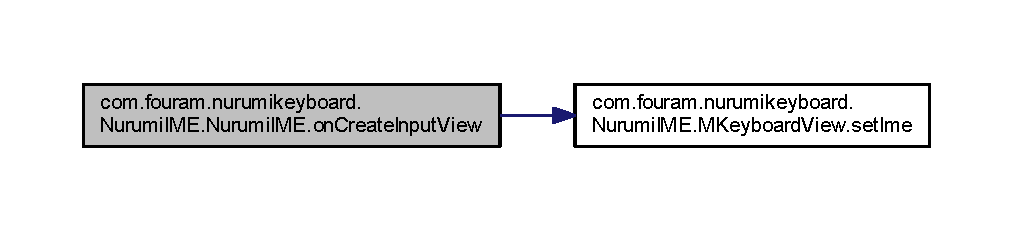
\includegraphics[width=350pt]{classcom_1_1fouram_1_1nurumikeyboard_1_1_nurumi_i_m_e_1_1_nurumi_i_m_e_a2cc9e540f1ef205df73a02b38842f2cf_cgraph}
\end{center}
\end{figure}


\hypertarget{classcom_1_1fouram_1_1nurumikeyboard_1_1_nurumi_i_m_e_1_1_nurumi_i_m_e_a8d8939dd9ba019a8ba3536f5529e105e}{}\index{com\+::fouram\+::nurumikeyboard\+::\+Nurumi\+I\+M\+E\+::\+Nurumi\+I\+M\+E@{com\+::fouram\+::nurumikeyboard\+::\+Nurumi\+I\+M\+E\+::\+Nurumi\+I\+M\+E}!on\+Evaluate\+Fullscreen\+Mode@{on\+Evaluate\+Fullscreen\+Mode}}
\index{on\+Evaluate\+Fullscreen\+Mode@{on\+Evaluate\+Fullscreen\+Mode}!com\+::fouram\+::nurumikeyboard\+::\+Nurumi\+I\+M\+E\+::\+Nurumi\+I\+M\+E@{com\+::fouram\+::nurumikeyboard\+::\+Nurumi\+I\+M\+E\+::\+Nurumi\+I\+M\+E}}
\subsubsection[{on\+Evaluate\+Fullscreen\+Mode}]{\setlength{\rightskip}{0pt plus 5cm}boolean com.\+fouram.\+nurumikeyboard.\+Nurumi\+I\+M\+E.\+Nurumi\+I\+M\+E.\+on\+Evaluate\+Fullscreen\+Mode (
\begin{DoxyParamCaption}
{}
\end{DoxyParamCaption}
)}\label{classcom_1_1fouram_1_1nurumikeyboard_1_1_nurumi_i_m_e_1_1_nurumi_i_m_e_a8d8939dd9ba019a8ba3536f5529e105e}


Definition at line 106 of file Nurumi\+I\+M\+E.\+java.


\begin{DoxyCode}
106                                               \{
107         \textcolor{keywordflow}{return} \textcolor{keyword}{false};
108     \}
\end{DoxyCode}
\hypertarget{classcom_1_1fouram_1_1nurumikeyboard_1_1_nurumi_i_m_e_1_1_nurumi_i_m_e_a539ed018248c5459a89e102ea4c8d5c5}{}\index{com\+::fouram\+::nurumikeyboard\+::\+Nurumi\+I\+M\+E\+::\+Nurumi\+I\+M\+E@{com\+::fouram\+::nurumikeyboard\+::\+Nurumi\+I\+M\+E\+::\+Nurumi\+I\+M\+E}!on\+Finish\+Gesture@{on\+Finish\+Gesture}}
\index{on\+Finish\+Gesture@{on\+Finish\+Gesture}!com\+::fouram\+::nurumikeyboard\+::\+Nurumi\+I\+M\+E\+::\+Nurumi\+I\+M\+E@{com\+::fouram\+::nurumikeyboard\+::\+Nurumi\+I\+M\+E\+::\+Nurumi\+I\+M\+E}}
\subsubsection[{on\+Finish\+Gesture}]{\setlength{\rightskip}{0pt plus 5cm}void com.\+fouram.\+nurumikeyboard.\+Nurumi\+I\+M\+E.\+Nurumi\+I\+M\+E.\+on\+Finish\+Gesture (
\begin{DoxyParamCaption}
\item[{int\mbox{[}$\,$\mbox{]}}]{motion}
\end{DoxyParamCaption}
)}\label{classcom_1_1fouram_1_1nurumikeyboard_1_1_nurumi_i_m_e_1_1_nurumi_i_m_e_a539ed018248c5459a89e102ea4c8d5c5}


Definition at line 130 of file Nurumi\+I\+M\+E.\+java.


\begin{DoxyCode}
130                                               \{
131         \textcolor{comment}{//Log.d("Gesture listener", "Listener executed!");}
132         \textcolor{keywordflow}{for}(\textcolor{keywordtype}{int} i = 0; i<\hyperlink{classcom_1_1fouram_1_1nurumikeyboard_1_1_nurumi_i_m_e_1_1_nurumi_i_m_e_a8da73863a9fc74d17aa828c3d6d7bf6b}{numFingers}; i++)
133             this.\hyperlink{classcom_1_1fouram_1_1nurumikeyboard_1_1_nurumi_i_m_e_1_1_nurumi_i_m_e_ac73ce0e0f969277597c8907855393ea8}{motion}[i] = \hyperlink{classcom_1_1fouram_1_1nurumikeyboard_1_1_nurumi_i_m_e_1_1_nurumi_i_m_e_ac73ce0e0f969277597c8907855393ea8}{motion}[i]; \textcolor{comment}{// get gesture input}
134         InputConnection ic = getCurrentInputConnection();
135         \textcolor{keywordflow}{if}(\hyperlink{classcom_1_1fouram_1_1nurumikeyboard_1_1_nurumi_i_m_e_1_1_nurumi_i_m_e_ac73ce0e0f969277597c8907855393ea8}{motion}[0] == 0)
136             ic.sendKeyEvent(\textcolor{keyword}{new} KeyEvent(KeyEvent.ACTION\_DOWN, KeyEvent.KEYCODE\_0));
137         \textcolor{keywordflow}{else}
138             ic.commitText(String.valueOf(\textcolor{stringliteral}{'��'}),1);
139     \}
\end{DoxyCode}


Here is the caller graph for this function\+:
\nopagebreak
\begin{figure}[H]
\begin{center}
\leavevmode
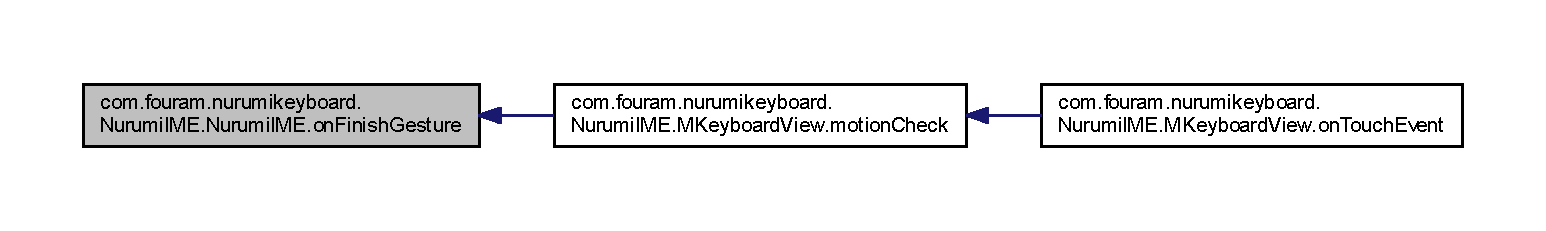
\includegraphics[width=350pt]{classcom_1_1fouram_1_1nurumikeyboard_1_1_nurumi_i_m_e_1_1_nurumi_i_m_e_a539ed018248c5459a89e102ea4c8d5c5_icgraph}
\end{center}
\end{figure}


\hypertarget{classcom_1_1fouram_1_1nurumikeyboard_1_1_nurumi_i_m_e_1_1_nurumi_i_m_e_a83c202c960e717ed80dd20c47e760a6c}{}\index{com\+::fouram\+::nurumikeyboard\+::\+Nurumi\+I\+M\+E\+::\+Nurumi\+I\+M\+E@{com\+::fouram\+::nurumikeyboard\+::\+Nurumi\+I\+M\+E\+::\+Nurumi\+I\+M\+E}!on\+Finish\+Input\+View@{on\+Finish\+Input\+View}}
\index{on\+Finish\+Input\+View@{on\+Finish\+Input\+View}!com\+::fouram\+::nurumikeyboard\+::\+Nurumi\+I\+M\+E\+::\+Nurumi\+I\+M\+E@{com\+::fouram\+::nurumikeyboard\+::\+Nurumi\+I\+M\+E\+::\+Nurumi\+I\+M\+E}}
\subsubsection[{on\+Finish\+Input\+View}]{\setlength{\rightskip}{0pt plus 5cm}void com.\+fouram.\+nurumikeyboard.\+Nurumi\+I\+M\+E.\+Nurumi\+I\+M\+E.\+on\+Finish\+Input\+View (
\begin{DoxyParamCaption}
\item[{boolean}]{finishing\+Input}
\end{DoxyParamCaption}
)}\label{classcom_1_1fouram_1_1nurumikeyboard_1_1_nurumi_i_m_e_1_1_nurumi_i_m_e_a83c202c960e717ed80dd20c47e760a6c}


Definition at line 52 of file Nurumi\+I\+M\+E.\+java.


\begin{DoxyCode}
52                                                           \{
53         super.onFinishInputView(finishingInput);
54     \}
\end{DoxyCode}
\hypertarget{classcom_1_1fouram_1_1nurumikeyboard_1_1_nurumi_i_m_e_1_1_nurumi_i_m_e_a187ecc78f108f4f394d63609503315bb}{}\index{com\+::fouram\+::nurumikeyboard\+::\+Nurumi\+I\+M\+E\+::\+Nurumi\+I\+M\+E@{com\+::fouram\+::nurumikeyboard\+::\+Nurumi\+I\+M\+E\+::\+Nurumi\+I\+M\+E}!on\+Show\+Input\+Requested@{on\+Show\+Input\+Requested}}
\index{on\+Show\+Input\+Requested@{on\+Show\+Input\+Requested}!com\+::fouram\+::nurumikeyboard\+::\+Nurumi\+I\+M\+E\+::\+Nurumi\+I\+M\+E@{com\+::fouram\+::nurumikeyboard\+::\+Nurumi\+I\+M\+E\+::\+Nurumi\+I\+M\+E}}
\subsubsection[{on\+Show\+Input\+Requested}]{\setlength{\rightskip}{0pt plus 5cm}boolean com.\+fouram.\+nurumikeyboard.\+Nurumi\+I\+M\+E.\+Nurumi\+I\+M\+E.\+on\+Show\+Input\+Requested (
\begin{DoxyParamCaption}
\item[{int}]{flags, }
\item[{boolean}]{config\+Change}
\end{DoxyParamCaption}
)}\label{classcom_1_1fouram_1_1nurumikeyboard_1_1_nurumi_i_m_e_1_1_nurumi_i_m_e_a187ecc78f108f4f394d63609503315bb}


Definition at line 81 of file Nurumi\+I\+M\+E.\+java.


\begin{DoxyCode}
81                                                                           \{
82         \textcolor{keywordflow}{return} \textcolor{keyword}{true};
83     \}
\end{DoxyCode}
\hypertarget{classcom_1_1fouram_1_1nurumikeyboard_1_1_nurumi_i_m_e_1_1_nurumi_i_m_e_a402ef1ca87efa5c183805ec36e249f5c}{}\index{com\+::fouram\+::nurumikeyboard\+::\+Nurumi\+I\+M\+E\+::\+Nurumi\+I\+M\+E@{com\+::fouram\+::nurumikeyboard\+::\+Nurumi\+I\+M\+E\+::\+Nurumi\+I\+M\+E}!on\+Update\+Extracting\+Visibility@{on\+Update\+Extracting\+Visibility}}
\index{on\+Update\+Extracting\+Visibility@{on\+Update\+Extracting\+Visibility}!com\+::fouram\+::nurumikeyboard\+::\+Nurumi\+I\+M\+E\+::\+Nurumi\+I\+M\+E@{com\+::fouram\+::nurumikeyboard\+::\+Nurumi\+I\+M\+E\+::\+Nurumi\+I\+M\+E}}
\subsubsection[{on\+Update\+Extracting\+Visibility}]{\setlength{\rightskip}{0pt plus 5cm}void com.\+fouram.\+nurumikeyboard.\+Nurumi\+I\+M\+E.\+Nurumi\+I\+M\+E.\+on\+Update\+Extracting\+Visibility (
\begin{DoxyParamCaption}
\item[{Editor\+Info}]{ei}
\end{DoxyParamCaption}
)}\label{classcom_1_1fouram_1_1nurumikeyboard_1_1_nurumi_i_m_e_1_1_nurumi_i_m_e_a402ef1ca87efa5c183805ec36e249f5c}


Definition at line 101 of file Nurumi\+I\+M\+E.\+java.


\begin{DoxyCode}
101                                                             \{
102         \hyperlink{classcom_1_1fouram_1_1nurumikeyboard_1_1_nurumi_i_m_e_1_1_nurumi_i_m_e_ab2bcb5ce607676ca73f5a64b6b087973}{setExtractViewShown}(\textcolor{keyword}{true});
103     \}
\end{DoxyCode}


Here is the call graph for this function\+:
\nopagebreak
\begin{figure}[H]
\begin{center}
\leavevmode
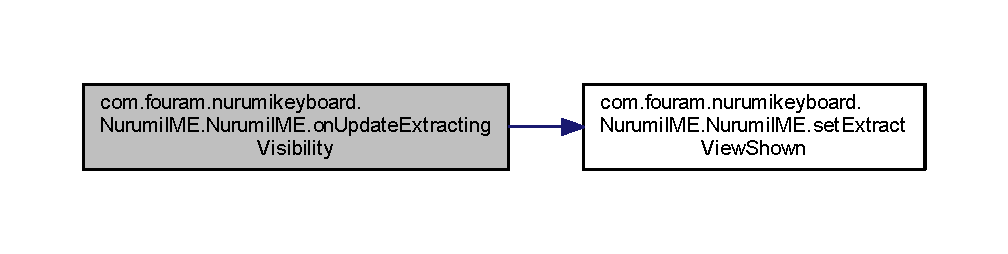
\includegraphics[width=350pt]{classcom_1_1fouram_1_1nurumikeyboard_1_1_nurumi_i_m_e_1_1_nurumi_i_m_e_a402ef1ca87efa5c183805ec36e249f5c_cgraph}
\end{center}
\end{figure}


\hypertarget{classcom_1_1fouram_1_1nurumikeyboard_1_1_nurumi_i_m_e_1_1_nurumi_i_m_e_a5917567be1a7c4f177968eb9cb130992}{}\index{com\+::fouram\+::nurumikeyboard\+::\+Nurumi\+I\+M\+E\+::\+Nurumi\+I\+M\+E@{com\+::fouram\+::nurumikeyboard\+::\+Nurumi\+I\+M\+E\+::\+Nurumi\+I\+M\+E}!on\+Window\+Hidden@{on\+Window\+Hidden}}
\index{on\+Window\+Hidden@{on\+Window\+Hidden}!com\+::fouram\+::nurumikeyboard\+::\+Nurumi\+I\+M\+E\+::\+Nurumi\+I\+M\+E@{com\+::fouram\+::nurumikeyboard\+::\+Nurumi\+I\+M\+E\+::\+Nurumi\+I\+M\+E}}
\subsubsection[{on\+Window\+Hidden}]{\setlength{\rightskip}{0pt plus 5cm}void com.\+fouram.\+nurumikeyboard.\+Nurumi\+I\+M\+E.\+Nurumi\+I\+M\+E.\+on\+Window\+Hidden (
\begin{DoxyParamCaption}
{}
\end{DoxyParamCaption}
)}\label{classcom_1_1fouram_1_1nurumikeyboard_1_1_nurumi_i_m_e_1_1_nurumi_i_m_e_a5917567be1a7c4f177968eb9cb130992}


Definition at line 94 of file Nurumi\+I\+M\+E.\+java.


\begin{DoxyCode}
94                                  \{
95         super.onWindowHidden();
96         \hyperlink{classcom_1_1fouram_1_1nurumikeyboard_1_1_nurumi_i_m_e_1_1_nurumi_i_m_e_a357ffb1d95223caceb27332fecdf4d5c}{mKeyboardView}.\hyperlink{classcom_1_1fouram_1_1nurumikeyboard_1_1_nurumi_i_m_e_1_1_m_keyboard_view_a536f8d1527df8c5013dc66d253ac5dae}{initialize}();
97     \}   
\end{DoxyCode}


Here is the call graph for this function\+:
\nopagebreak
\begin{figure}[H]
\begin{center}
\leavevmode
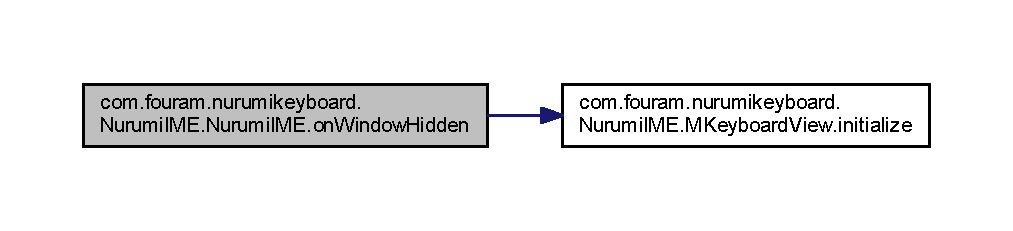
\includegraphics[width=350pt]{classcom_1_1fouram_1_1nurumikeyboard_1_1_nurumi_i_m_e_1_1_nurumi_i_m_e_a5917567be1a7c4f177968eb9cb130992_cgraph}
\end{center}
\end{figure}


\hypertarget{classcom_1_1fouram_1_1nurumikeyboard_1_1_nurumi_i_m_e_1_1_nurumi_i_m_e_ab2bcb5ce607676ca73f5a64b6b087973}{}\index{com\+::fouram\+::nurumikeyboard\+::\+Nurumi\+I\+M\+E\+::\+Nurumi\+I\+M\+E@{com\+::fouram\+::nurumikeyboard\+::\+Nurumi\+I\+M\+E\+::\+Nurumi\+I\+M\+E}!set\+Extract\+View\+Shown@{set\+Extract\+View\+Shown}}
\index{set\+Extract\+View\+Shown@{set\+Extract\+View\+Shown}!com\+::fouram\+::nurumikeyboard\+::\+Nurumi\+I\+M\+E\+::\+Nurumi\+I\+M\+E@{com\+::fouram\+::nurumikeyboard\+::\+Nurumi\+I\+M\+E\+::\+Nurumi\+I\+M\+E}}
\subsubsection[{set\+Extract\+View\+Shown}]{\setlength{\rightskip}{0pt plus 5cm}void com.\+fouram.\+nurumikeyboard.\+Nurumi\+I\+M\+E.\+Nurumi\+I\+M\+E.\+set\+Extract\+View\+Shown (
\begin{DoxyParamCaption}
\item[{boolean}]{shown}
\end{DoxyParamCaption}
)}\label{classcom_1_1fouram_1_1nurumikeyboard_1_1_nurumi_i_m_e_1_1_nurumi_i_m_e_ab2bcb5ce607676ca73f5a64b6b087973}


Definition at line 116 of file Nurumi\+I\+M\+E.\+java.


\begin{DoxyCode}
116                                                    \{
117         super.setExtractViewShown(\textcolor{keyword}{true});
118     \}
\end{DoxyCode}


Here is the caller graph for this function\+:
\nopagebreak
\begin{figure}[H]
\begin{center}
\leavevmode
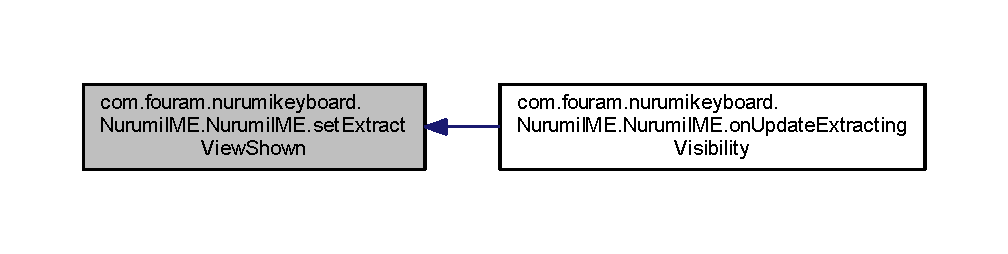
\includegraphics[width=350pt]{classcom_1_1fouram_1_1nurumikeyboard_1_1_nurumi_i_m_e_1_1_nurumi_i_m_e_ab2bcb5ce607676ca73f5a64b6b087973_icgraph}
\end{center}
\end{figure}




\subsection{Member Data Documentation}
\hypertarget{classcom_1_1fouram_1_1nurumikeyboard_1_1_nurumi_i_m_e_1_1_nurumi_i_m_e_adf766bc5635fcf0dd670402d172e45ba}{}\index{com\+::fouram\+::nurumikeyboard\+::\+Nurumi\+I\+M\+E\+::\+Nurumi\+I\+M\+E@{com\+::fouram\+::nurumikeyboard\+::\+Nurumi\+I\+M\+E\+::\+Nurumi\+I\+M\+E}!entire\+View@{entire\+View}}
\index{entire\+View@{entire\+View}!com\+::fouram\+::nurumikeyboard\+::\+Nurumi\+I\+M\+E\+::\+Nurumi\+I\+M\+E@{com\+::fouram\+::nurumikeyboard\+::\+Nurumi\+I\+M\+E\+::\+Nurumi\+I\+M\+E}}
\subsubsection[{entire\+View}]{\setlength{\rightskip}{0pt plus 5cm}View com.\+fouram.\+nurumikeyboard.\+Nurumi\+I\+M\+E.\+Nurumi\+I\+M\+E.\+entire\+View\hspace{0.3cm}{\ttfamily [private]}}\label{classcom_1_1fouram_1_1nurumikeyboard_1_1_nurumi_i_m_e_1_1_nurumi_i_m_e_adf766bc5635fcf0dd670402d172e45ba}


Definition at line 47 of file Nurumi\+I\+M\+E.\+java.

\hypertarget{classcom_1_1fouram_1_1nurumikeyboard_1_1_nurumi_i_m_e_1_1_nurumi_i_m_e_a9b39dd4573a5446f50b56ae0f0beba4d}{}\index{com\+::fouram\+::nurumikeyboard\+::\+Nurumi\+I\+M\+E\+::\+Nurumi\+I\+M\+E@{com\+::fouram\+::nurumikeyboard\+::\+Nurumi\+I\+M\+E\+::\+Nurumi\+I\+M\+E}!F\+I\+V\+E\+\_\+\+F\+I\+N\+G\+E\+R\+S@{F\+I\+V\+E\+\_\+\+F\+I\+N\+G\+E\+R\+S}}
\index{F\+I\+V\+E\+\_\+\+F\+I\+N\+G\+E\+R\+S@{F\+I\+V\+E\+\_\+\+F\+I\+N\+G\+E\+R\+S}!com\+::fouram\+::nurumikeyboard\+::\+Nurumi\+I\+M\+E\+::\+Nurumi\+I\+M\+E@{com\+::fouram\+::nurumikeyboard\+::\+Nurumi\+I\+M\+E\+::\+Nurumi\+I\+M\+E}}
\subsubsection[{F\+I\+V\+E\+\_\+\+F\+I\+N\+G\+E\+R\+S}]{\setlength{\rightskip}{0pt plus 5cm}final int com.\+fouram.\+nurumikeyboard.\+Nurumi\+I\+M\+E.\+Nurumi\+I\+M\+E.\+F\+I\+V\+E\+\_\+\+F\+I\+N\+G\+E\+R\+S = 5\hspace{0.3cm}{\ttfamily [private]}}\label{classcom_1_1fouram_1_1nurumikeyboard_1_1_nurumi_i_m_e_1_1_nurumi_i_m_e_a9b39dd4573a5446f50b56ae0f0beba4d}


Definition at line 44 of file Nurumi\+I\+M\+E.\+java.

\hypertarget{classcom_1_1fouram_1_1nurumikeyboard_1_1_nurumi_i_m_e_1_1_nurumi_i_m_e_a357ffb1d95223caceb27332fecdf4d5c}{}\index{com\+::fouram\+::nurumikeyboard\+::\+Nurumi\+I\+M\+E\+::\+Nurumi\+I\+M\+E@{com\+::fouram\+::nurumikeyboard\+::\+Nurumi\+I\+M\+E\+::\+Nurumi\+I\+M\+E}!m\+Keyboard\+View@{m\+Keyboard\+View}}
\index{m\+Keyboard\+View@{m\+Keyboard\+View}!com\+::fouram\+::nurumikeyboard\+::\+Nurumi\+I\+M\+E\+::\+Nurumi\+I\+M\+E@{com\+::fouram\+::nurumikeyboard\+::\+Nurumi\+I\+M\+E\+::\+Nurumi\+I\+M\+E}}
\subsubsection[{m\+Keyboard\+View}]{\setlength{\rightskip}{0pt plus 5cm}{\bf M\+Keyboard\+View} com.\+fouram.\+nurumikeyboard.\+Nurumi\+I\+M\+E.\+Nurumi\+I\+M\+E.\+m\+Keyboard\+View\hspace{0.3cm}{\ttfamily [private]}}\label{classcom_1_1fouram_1_1nurumikeyboard_1_1_nurumi_i_m_e_1_1_nurumi_i_m_e_a357ffb1d95223caceb27332fecdf4d5c}


Definition at line 49 of file Nurumi\+I\+M\+E.\+java.

\hypertarget{classcom_1_1fouram_1_1nurumikeyboard_1_1_nurumi_i_m_e_1_1_nurumi_i_m_e_ac73ce0e0f969277597c8907855393ea8}{}\index{com\+::fouram\+::nurumikeyboard\+::\+Nurumi\+I\+M\+E\+::\+Nurumi\+I\+M\+E@{com\+::fouram\+::nurumikeyboard\+::\+Nurumi\+I\+M\+E\+::\+Nurumi\+I\+M\+E}!motion@{motion}}
\index{motion@{motion}!com\+::fouram\+::nurumikeyboard\+::\+Nurumi\+I\+M\+E\+::\+Nurumi\+I\+M\+E@{com\+::fouram\+::nurumikeyboard\+::\+Nurumi\+I\+M\+E\+::\+Nurumi\+I\+M\+E}}
\subsubsection[{motion}]{\setlength{\rightskip}{0pt plus 5cm}int \mbox{[}$\,$\mbox{]} com.\+fouram.\+nurumikeyboard.\+Nurumi\+I\+M\+E.\+Nurumi\+I\+M\+E.\+motion\hspace{0.3cm}{\ttfamily [private]}}\label{classcom_1_1fouram_1_1nurumikeyboard_1_1_nurumi_i_m_e_1_1_nurumi_i_m_e_ac73ce0e0f969277597c8907855393ea8}


Definition at line 50 of file Nurumi\+I\+M\+E.\+java.

\hypertarget{classcom_1_1fouram_1_1nurumikeyboard_1_1_nurumi_i_m_e_1_1_nurumi_i_m_e_a8da73863a9fc74d17aa828c3d6d7bf6b}{}\index{com\+::fouram\+::nurumikeyboard\+::\+Nurumi\+I\+M\+E\+::\+Nurumi\+I\+M\+E@{com\+::fouram\+::nurumikeyboard\+::\+Nurumi\+I\+M\+E\+::\+Nurumi\+I\+M\+E}!num\+Fingers@{num\+Fingers}}
\index{num\+Fingers@{num\+Fingers}!com\+::fouram\+::nurumikeyboard\+::\+Nurumi\+I\+M\+E\+::\+Nurumi\+I\+M\+E@{com\+::fouram\+::nurumikeyboard\+::\+Nurumi\+I\+M\+E\+::\+Nurumi\+I\+M\+E}}
\subsubsection[{num\+Fingers}]{\setlength{\rightskip}{0pt plus 5cm}int com.\+fouram.\+nurumikeyboard.\+Nurumi\+I\+M\+E.\+Nurumi\+I\+M\+E.\+num\+Fingers\hspace{0.3cm}{\ttfamily [private]}}\label{classcom_1_1fouram_1_1nurumikeyboard_1_1_nurumi_i_m_e_1_1_nurumi_i_m_e_a8da73863a9fc74d17aa828c3d6d7bf6b}


Definition at line 46 of file Nurumi\+I\+M\+E.\+java.

\hypertarget{classcom_1_1fouram_1_1nurumikeyboard_1_1_nurumi_i_m_e_1_1_nurumi_i_m_e_afcdaac68a2da0f716da9b2ea582ea2ad}{}\index{com\+::fouram\+::nurumikeyboard\+::\+Nurumi\+I\+M\+E\+::\+Nurumi\+I\+M\+E@{com\+::fouram\+::nurumikeyboard\+::\+Nurumi\+I\+M\+E\+::\+Nurumi\+I\+M\+E}!T\+E\+N\+\_\+\+F\+I\+N\+G\+E\+R\+S@{T\+E\+N\+\_\+\+F\+I\+N\+G\+E\+R\+S}}
\index{T\+E\+N\+\_\+\+F\+I\+N\+G\+E\+R\+S@{T\+E\+N\+\_\+\+F\+I\+N\+G\+E\+R\+S}!com\+::fouram\+::nurumikeyboard\+::\+Nurumi\+I\+M\+E\+::\+Nurumi\+I\+M\+E@{com\+::fouram\+::nurumikeyboard\+::\+Nurumi\+I\+M\+E\+::\+Nurumi\+I\+M\+E}}
\subsubsection[{T\+E\+N\+\_\+\+F\+I\+N\+G\+E\+R\+S}]{\setlength{\rightskip}{0pt plus 5cm}final int com.\+fouram.\+nurumikeyboard.\+Nurumi\+I\+M\+E.\+Nurumi\+I\+M\+E.\+T\+E\+N\+\_\+\+F\+I\+N\+G\+E\+R\+S = 10\hspace{0.3cm}{\ttfamily [private]}}\label{classcom_1_1fouram_1_1nurumikeyboard_1_1_nurumi_i_m_e_1_1_nurumi_i_m_e_afcdaac68a2da0f716da9b2ea582ea2ad}


Definition at line 45 of file Nurumi\+I\+M\+E.\+java.

\hypertarget{classcom_1_1fouram_1_1nurumikeyboard_1_1_nurumi_i_m_e_1_1_nurumi_i_m_e_addc58b240728adb839c40fa65e1b89bb}{}\index{com\+::fouram\+::nurumikeyboard\+::\+Nurumi\+I\+M\+E\+::\+Nurumi\+I\+M\+E@{com\+::fouram\+::nurumikeyboard\+::\+Nurumi\+I\+M\+E\+::\+Nurumi\+I\+M\+E}!vg@{vg}}
\index{vg@{vg}!com\+::fouram\+::nurumikeyboard\+::\+Nurumi\+I\+M\+E\+::\+Nurumi\+I\+M\+E@{com\+::fouram\+::nurumikeyboard\+::\+Nurumi\+I\+M\+E\+::\+Nurumi\+I\+M\+E}}
\subsubsection[{vg}]{\setlength{\rightskip}{0pt plus 5cm}View\+Group com.\+fouram.\+nurumikeyboard.\+Nurumi\+I\+M\+E.\+Nurumi\+I\+M\+E.\+vg\hspace{0.3cm}{\ttfamily [private]}}\label{classcom_1_1fouram_1_1nurumikeyboard_1_1_nurumi_i_m_e_1_1_nurumi_i_m_e_addc58b240728adb839c40fa65e1b89bb}


Definition at line 48 of file Nurumi\+I\+M\+E.\+java.



The documentation for this class was generated from the following file\+:\begin{DoxyCompactItemize}
\item 
src/com/fouram/nurumikeyboard/\+Nurumi\+I\+M\+E/\hyperlink{_nurumi_i_m_e_8java}{Nurumi\+I\+M\+E.\+java}\end{DoxyCompactItemize}

\hypertarget{classcom_1_1fouram_1_1nurumikeyboard_1_1_nurumi_i_m_e_1_1_m_keyboard_view_1_1_pt_id_linked_with_pt_index}{}\section{com.\+fouram.\+nurumikeyboard.\+Nurumi\+I\+M\+E.\+M\+Keyboard\+View.\+Pt\+Id\+Linked\+With\+Pt\+Index Class Reference}
\label{classcom_1_1fouram_1_1nurumikeyboard_1_1_nurumi_i_m_e_1_1_m_keyboard_view_1_1_pt_id_linked_with_pt_index}\index{com.\+fouram.\+nurumikeyboard.\+Nurumi\+I\+M\+E.\+M\+Keyboard\+View.\+Pt\+Id\+Linked\+With\+Pt\+Index@{com.\+fouram.\+nurumikeyboard.\+Nurumi\+I\+M\+E.\+M\+Keyboard\+View.\+Pt\+Id\+Linked\+With\+Pt\+Index}}


Collaboration diagram for com.\+fouram.\+nurumikeyboard.\+Nurumi\+I\+M\+E.\+M\+Keyboard\+View.\+Pt\+Id\+Linked\+With\+Pt\+Index\+:
\nopagebreak
\begin{figure}[H]
\begin{center}
\leavevmode
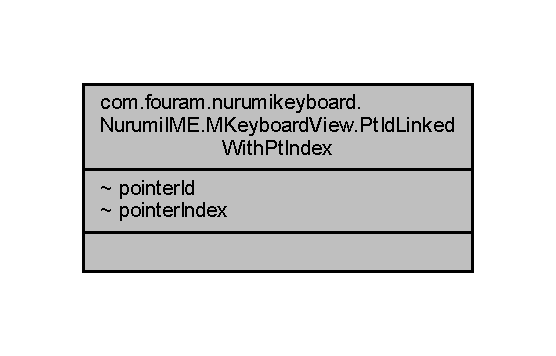
\includegraphics[width=267pt]{classcom_1_1fouram_1_1nurumikeyboard_1_1_nurumi_i_m_e_1_1_m_keyboard_view_1_1_pt_id_linked_with_pt_index__coll__graph}
\end{center}
\end{figure}


\subsection{Detailed Description}
\hyperlink{namespacecom_1_1fouram_1_1nurumikeyboard_1_1_nurumi_i_m_e}{com.\+fouram.\+nurumikeyboard.\+Nurumi\+I\+M\+E} ~\newline
 �� \hyperlink{_m_keyboard_view_8java}{M\+Keyboard\+View.\+java} \hypertarget{classcom_1_1fouram_1_1nurumikeyboard_1_1_nurumi_i_m_e_1_1_m_keyboard_view_1_1_pt_id_linked_with_pt_index_Class}{}\subsection{information}\label{classcom_1_1fouram_1_1nurumikeyboard_1_1_nurumi_i_m_e_1_1_m_keyboard_view_1_1_pt_id_linked_with_pt_index_Class}
\begin{TabularC}{2}
\hline
\rowcolor{lightgray}\PBS\centering {\bf Item }&{\bf Contents  }\\\cline{1-2}
\PBS\centering Company &4\+:00 A.\+M. \\\cline{1-2}
\PBS\centering Author &Park, Hyung Soon \\\cline{1-2}
\PBS\centering Date &2015. 3. 26. \\\cline{1-2}
\end{TabularC}
\hypertarget{classcom_1_1fouram_1_1nurumikeyboard_1_1_nurumi_i_m_e_1_1_m_keyboard_view_1_1_pt_id_linked_with_pt_index_Description}{}\subsection{Description}\label{classcom_1_1fouram_1_1nurumikeyboard_1_1_nurumi_i_m_e_1_1_m_keyboard_view_1_1_pt_id_linked_with_pt_index_Description}

\begin{DoxyItemize}
\item This class will bind pointer\+I\+D with pointer\+Index 
\end{DoxyItemize}

Definition at line 95 of file M\+Keyboard\+View.\+java.



The documentation for this class was generated from the following file\+:\begin{DoxyCompactItemize}
\item 
src/com/fouram/nurumikeyboard/\+Nurumi\+I\+M\+E/\hyperlink{_m_keyboard_view_8java}{M\+Keyboard\+View.\+java}\end{DoxyCompactItemize}

\chapter{File Documentation}
\hypertarget{_m_keyboard_view_8java}{}\section{src/com/fouram/nurumikeyboard/\+Nurumi\+I\+M\+E/\+M\+Keyboard\+View.java File Reference}
\label{_m_keyboard_view_8java}\index{src/com/fouram/nurumikeyboard/\+Nurumi\+I\+M\+E/\+M\+Keyboard\+View.\+java@{src/com/fouram/nurumikeyboard/\+Nurumi\+I\+M\+E/\+M\+Keyboard\+View.\+java}}
\subsection*{Classes}
\begin{DoxyCompactItemize}
\item 
class \hyperlink{classcom_1_1fouram_1_1nurumikeyboard_1_1_nurumi_i_m_e_1_1_m_keyboard_view}{com.\+fouram.\+nurumikeyboard.\+Nurumi\+I\+M\+E.\+M\+Keyboard\+View}
\item 
class \hyperlink{classcom_1_1fouram_1_1nurumikeyboard_1_1_nurumi_i_m_e_1_1_m_keyboard_view_1_1_circle_linked_with_pt_id}{com.\+fouram.\+nurumikeyboard.\+Nurumi\+I\+M\+E.\+M\+Keyboard\+View.\+Circle\+Linked\+With\+Pt\+Id}
\item 
class \hyperlink{classcom_1_1fouram_1_1nurumikeyboard_1_1_nurumi_i_m_e_1_1_m_keyboard_view_1_1_pt_id_linked_with_pt_index}{com.\+fouram.\+nurumikeyboard.\+Nurumi\+I\+M\+E.\+M\+Keyboard\+View.\+Pt\+Id\+Linked\+With\+Pt\+Index}
\end{DoxyCompactItemize}
\subsection*{Packages}
\begin{DoxyCompactItemize}
\item 
package \hyperlink{namespacecom_1_1fouram_1_1nurumikeyboard_1_1_nurumi_i_m_e}{com.\+fouram.\+nurumikeyboard.\+Nurumi\+I\+M\+E}
\end{DoxyCompactItemize}

\hypertarget{_nurumi_i_m_e_8java}{}\section{src/com/fouram/nurumikeyboard/\+Nurumi\+I\+M\+E/\+Nurumi\+I\+M\+E.java File Reference}
\label{_nurumi_i_m_e_8java}\index{src/com/fouram/nurumikeyboard/\+Nurumi\+I\+M\+E/\+Nurumi\+I\+M\+E.\+java@{src/com/fouram/nurumikeyboard/\+Nurumi\+I\+M\+E/\+Nurumi\+I\+M\+E.\+java}}
\subsection*{Classes}
\begin{DoxyCompactItemize}
\item 
class \hyperlink{classcom_1_1fouram_1_1nurumikeyboard_1_1_nurumi_i_m_e_1_1_nurumi_i_m_e}{com.\+fouram.\+nurumikeyboard.\+Nurumi\+I\+M\+E.\+Nurumi\+I\+M\+E}
\end{DoxyCompactItemize}
\subsection*{Packages}
\begin{DoxyCompactItemize}
\item 
package \hyperlink{namespacecom_1_1fouram_1_1nurumikeyboard_1_1_nurumi_i_m_e}{com.\+fouram.\+nurumikeyboard.\+Nurumi\+I\+M\+E}
\end{DoxyCompactItemize}

%--- End generated contents ---

% Index
\backmatter
\newpage
\phantomsection
\clearemptydoublepage
\addcontentsline{toc}{chapter}{Index}
\printindex

\end{document}
